\chapter{Exercise 2: Function Estimation and Time Series Prediction}

\section{Support vector machine for function estimation}
\textbf{Construct a dataset where a linear kernel is better than any other kernel (around 20
	data points). What is the influence of e (try small values such as 0:10; 0:25; 0:50;..)
	and of Bound (try larger increments such as 0:01; 0:10; 1; 10; 100). Where does the
	sparsity property come in?}

The parameter $\epsilon$ controls the number of support vectors that the model takes to build the regression function. This in-turn determines width of the margin to fit the training data. Lower the value of $\epsilon$, higher the number of support vectors taken by that the model and vice versa. If $\epsilon$ values keeps increasing, the regressor fails to fit all the training data. This can be observed from the figures \ref{fig:lin_E=0.1_B=0.1}, \ref{fig:lin_E=0.3_B=0.1} and \ref{fig:lin_E=0.5_B=0.1} for a fixed bound value. On the other hand, we fix the value of $\epsilon$ and explore the regressor's performance for various values of bound. From figures \ref{fig:lin_E=0.15_B=0.01}, \ref{fig:lin_E=0.15_B=0.1} and \ref{fig:lin_E=0.15_B=10}m it can seen that the model performs poorly for lower value of bound and fits all the training data for higher value of bound.  Further increasing the bound value can cause the model to over-fit. It can be said that the bound is a trade-off between the error and model confidence. Sparsity comes into the picture when the model estimates better with less data points on unseen data. There won't be any sparseness in the model when it uses all the data points as support vectors. It is only possible for some optimal bound and $\epsilon$ say (0.15 and 0.1) as seen from figure \ref{fig:lin_E=0.15_B=0.1}.
\begin{figure}[ht]
	\centering
	\begin{subfigure}[b]{0.3\textwidth}
		\centering
		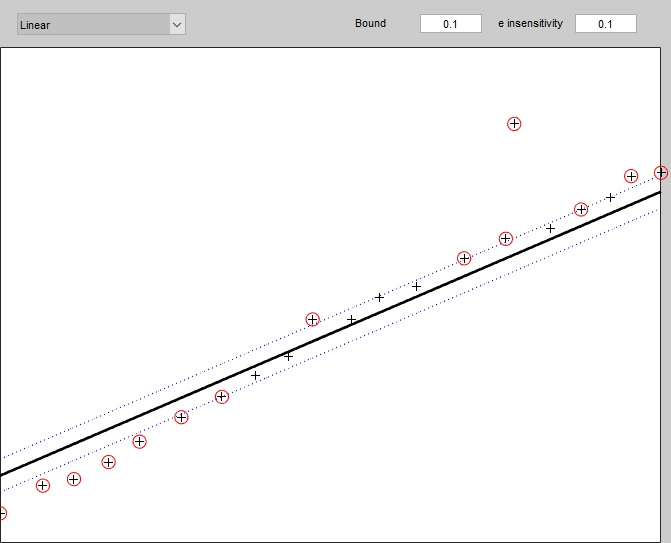
\includegraphics[width = 0.85\textwidth]{Exercise2/Report/Ex2.1_E=0.1_B=0.1}
		\caption{$\epsilon = 0.1$, Bound = 0.1 }\label{fig:lin_E=0.1_B=0.1}
	\end{subfigure}%
	\begin{subfigure}[b]{0.3\textwidth}
		\centering
		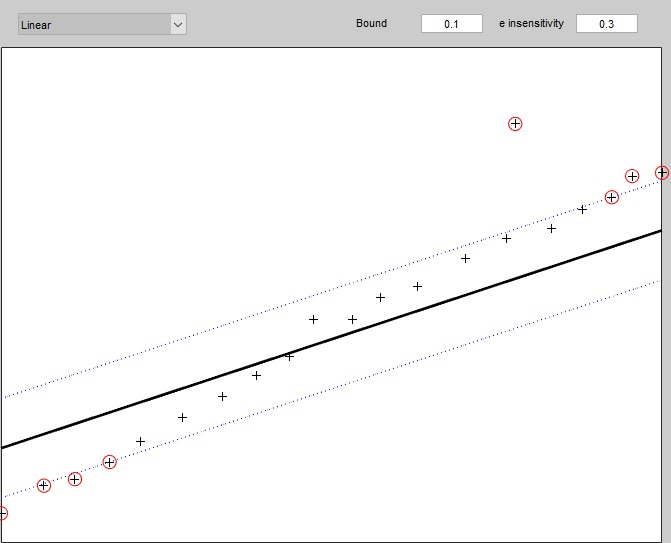
\includegraphics[width = 0.85\textwidth]{Exercise2/Report/Ex2.1_E=0.3_B=0.1}
		\caption{$\epsilon = 0.3$, Bound = 0.1 }\label{fig:lin_E=0.3_B=0.1}
	\end{subfigure}%
	\begin{subfigure}[b]{0.3\textwidth}
		\centering
		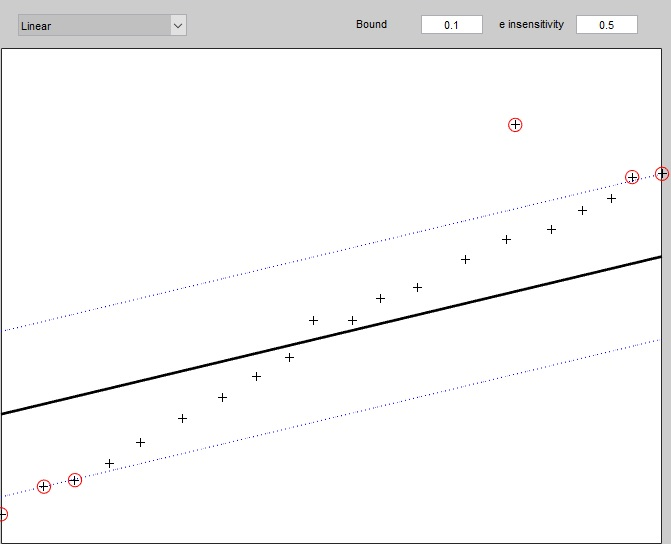
\includegraphics[width = 0.85\textwidth]{Exercise2/Report/Ex2.1_E=0.5_B=0.1}
		\caption{$\epsilon = 0.5$, Bound = 0.1 }\label{fig:lin_E=0.5_B=0.1}
	\end{subfigure}
	\begin{subfigure}[b]{0.3\textwidth}
		\centering
		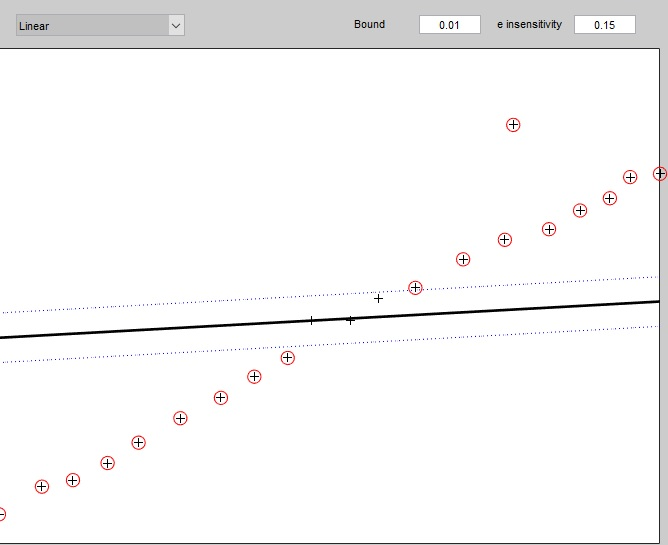
\includegraphics[width = 0.85\textwidth]{Exercise2/Report/Ex2.1_E=0.15_B=0.01}
		\caption{$\epsilon = 0.15$, Bound = 0.01 }\label{fig:lin_E=0.15_B=0.01}
	\end{subfigure}%
	\begin{subfigure}[b]{0.3\textwidth}
		\centering
		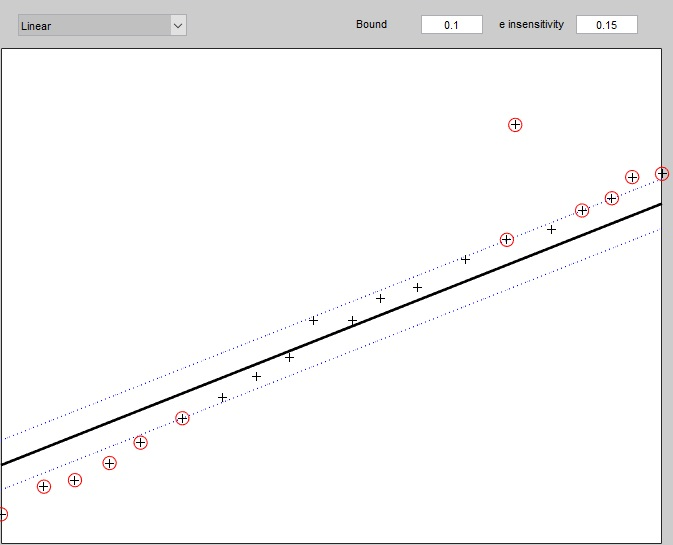
\includegraphics[width = 0.85\textwidth]{Exercise2/Report/Ex2.1_E=0.15_B=0.1}
		\caption{$\epsilon = 0.15$, Bound = 0.1 }\label{fig:lin_E=0.15_B=0.1}
	\end{subfigure}%
	\begin{subfigure}[b]{0.3\textwidth}
		\centering
		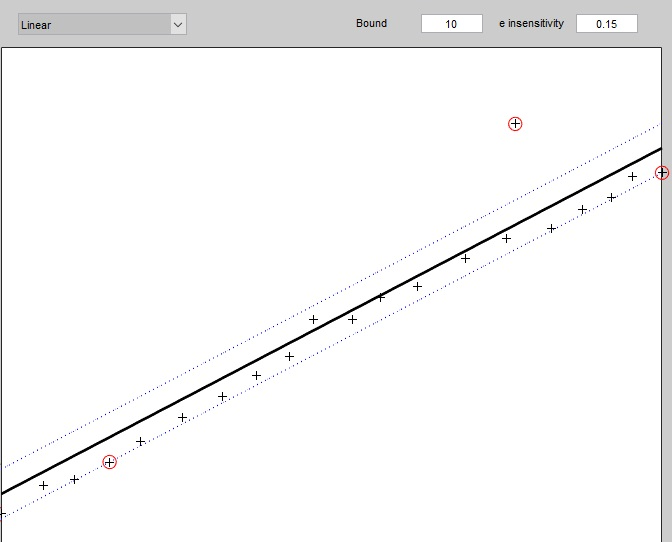
\includegraphics[width = 0.85\textwidth]{Exercise2/Report/Ex2.1_E=0.15_B=10}
		\caption{$\epsilon = 0.15$, Bound = 10 }\label{fig:lin_E=0.15_B=10}
	\end{subfigure}
	\caption{SVM for Regression using Linear Kernel: demo \texttt{uiregress}. All the figures have same data points and performance of the regressor for different values of $\epsilon$ and bound are observed}
	\label{fig:uiregress_Linear}
\end{figure}\\
\textbf{Construct a more challenging dataset (around 20 data points). Which kernel is best
	suited for your dataset? Motivate why.}

Figure \ref{fig:uiregress_Kernels} shows the performance of the SVM regressor with different kernels on a challenging dataset for fixed values of $\epsilon$ and bound. Linear kernel as seen in figure \ref{fig:lin_E=0.6_B=inf} doesn't perform well. Polynomial kernels as seen from figures \ref{fig:Poly_deg=3_E=1_B=0.6} and \ref{fig:Poly_deg=5_E=1_B=0.6}, for degree = 3 doesn't perform well but for degree = 5 generalizes better. If the polynomial degree is increase the model over-fits. Figures \ref{fig:RBF_sig=0.05_E=1_B=0.6}, \ref{fig:RBF_sig=0.1_E=1_B=0.6} and \ref{fig:RBF_sig=1_E=1_B=0.6} shows the regressor with RBF kernel for various $\sigma^2$ values. For very lower values of $\sigma^2$, the model over-fits but for higher values the model gives a linear estimate. Therefore, for a value of $\sigma^2$ = 0.1, the model generalizes better. Overall the regressor with RBF kernel performs betters as it learns complex patterns of data better compared to a polynomial kernel.
\begin{figure}[ht]
	\centering
	\begin{subfigure}[b]{0.35\textwidth}
		\centering
		\captionsetup{width=0.8\linewidth}
		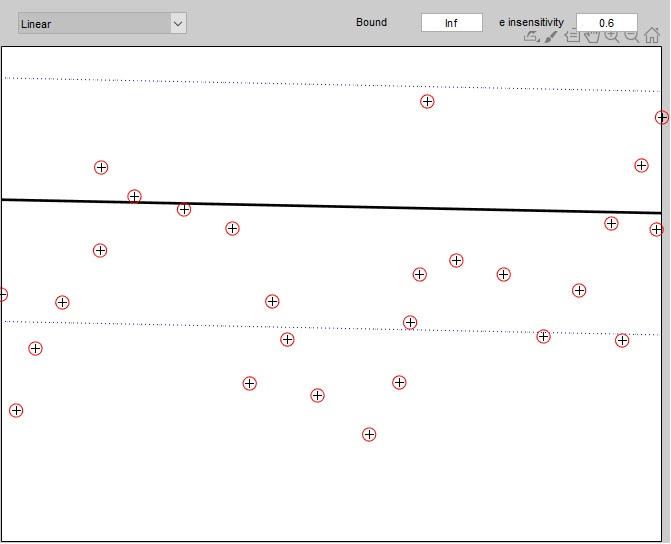
\includegraphics[width = 0.85\textwidth]{Exercise2/Report/Ex2.1_E=0.6_B=inf}
		\caption{Linear : $\epsilon = 0.6$, Bound = inf }\label{fig:lin_E=0.6_B=inf}
	\end{subfigure}%
	\begin{subfigure}[b]{0.35\textwidth}
		\centering
		\captionsetup{width=0.8\linewidth}
		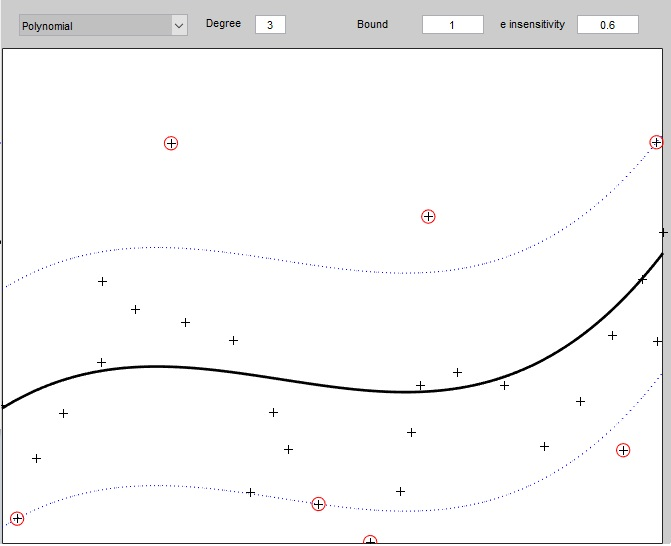
\includegraphics[width = 0.85\textwidth]{Exercise2/Report/Ex2.1_Poly_deg=3_E=1_B=0.6}
		\caption{Poly : degree =3, $\epsilon = 1$, Bound = 0.6 }\label{fig:Poly_deg=3_E=1_B=0.6}
	\end{subfigure}%
	\begin{subfigure}[b]{0.35\textwidth}
		\centering
		\captionsetup{width=0.8\linewidth}
		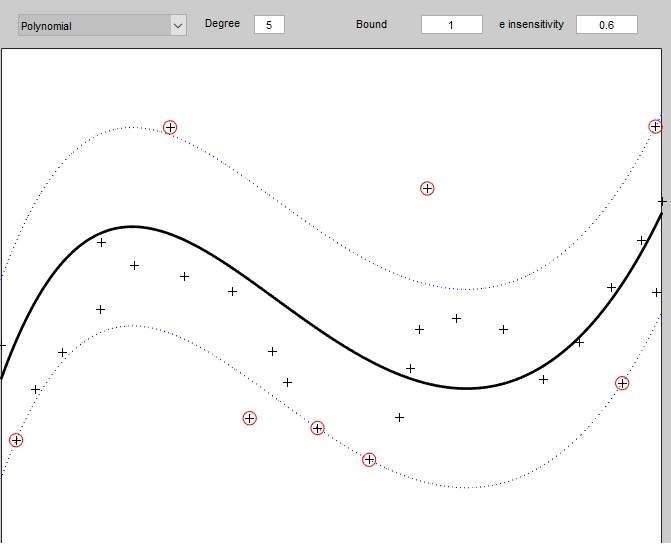
\includegraphics[width = 0.85\textwidth]{Exercise2/Report/Ex2.1_Poly_deg=5_E=1_B=0.6}
		\caption{Poly : degree =5, $\epsilon = 1$, Bound = 0.6 }\label{fig:Poly_deg=5_E=1_B=0.6}
	\end{subfigure}
	\begin{subfigure}[b]{0.35\textwidth}
		\centering
		\captionsetup{width=0.8\linewidth}
		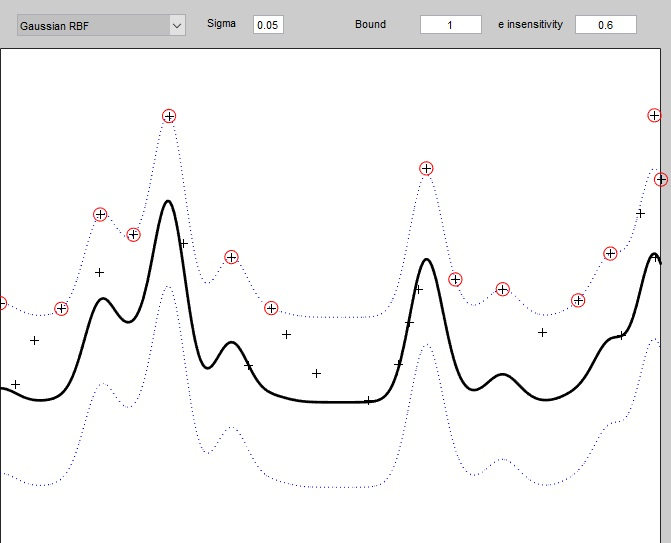
\includegraphics[width = 0.85\textwidth]{Exercise2/Report/Ex2.1_RBF_sig=0.05_E=1_B=0.6}
		\caption{RBF : $\sigma^2 = 0.05$ $\epsilon = 0.15$, Bound = 0.01 }\label{fig:RBF_sig=0.05_E=1_B=0.6}
	\end{subfigure}%
	\begin{subfigure}[b]{0.35\textwidth}
		\centering
		\captionsetup{width=0.8\linewidth}
		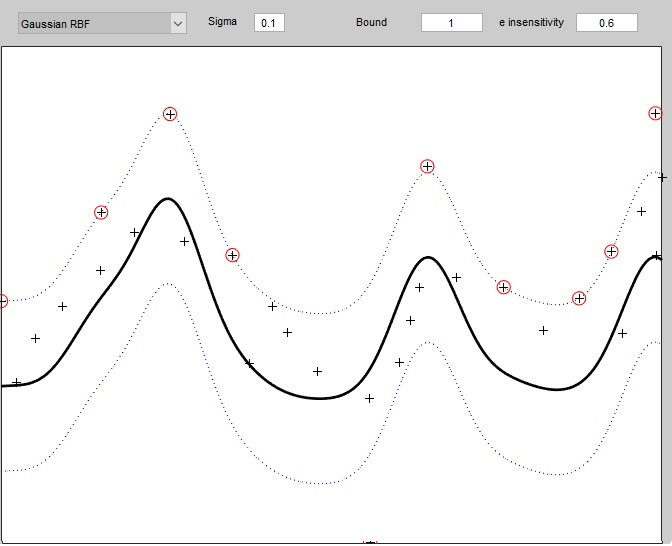
\includegraphics[width = 0.85\textwidth]{Exercise2/Report/Ex2.1_RBF_sig=0.1_E=1_B=0.6}
		\caption{RBF : $\sigma^2 = 0.1$ $\epsilon = 0.15$, Bound = 0.01 }\label{fig:RBF_sig=0.1_E=1_B=0.6}
	\end{subfigure}%
	\begin{subfigure}[b]{0.35\textwidth}
		\centering
		\captionsetup{width=0.8\linewidth}
		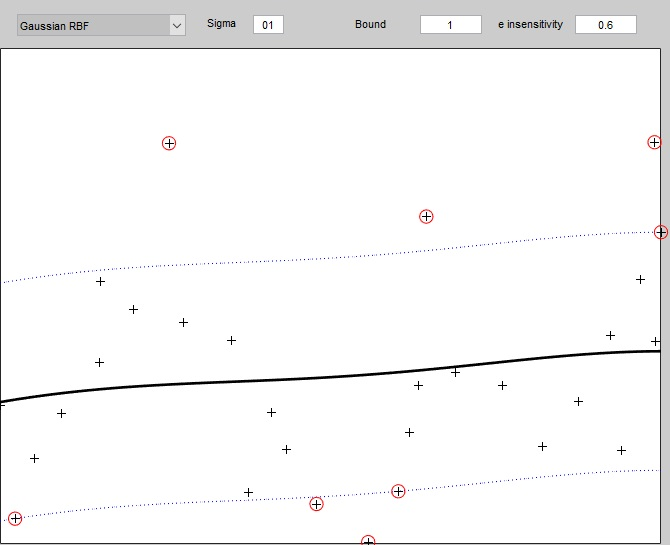
\includegraphics[width = 0.85\textwidth]{Exercise2/Report/Ex2.1_RBF_sig=1_E=1_B=0.6}
		\caption{RBF : $\sigma^2 = 1$ $\epsilon = 0.15$, Bound = 0.01 }\label{fig:RBF_sig=1_E=1_B=0.6}
	\end{subfigure}
	\caption{SVM for Regression using Linear, Polynomial and RBF Kernels: demo \texttt{uiregress}. }
	\label{fig:uiregress_Kernels}
\end{figure}\\
\textbf{In what respect is SVM regression different from a classical least squares fit?}

The difference in SVM regression and classical least squares is seen in loss function. Classical least squares use a L2 (squared) loss where as SVR uses a L1 loss with a threshold $\epsilon$. The observations outside this $\epsilon$ threshold is considered as points contributing to error.
\section{The sinc function}
\subsection{Regression of the sinc function}
\textbf{Try out a range of different gam and sig2 parameter values (e.g., gam = 10; $10^3$; $10^6$
	and sig2 = 0:01; 1; 100) and visualize the resulting function estimation on the test
	set data points. Discuss the resulting function estimation. Report the mean squared
	error for every combination ($\gamma$, $\sigma^2$).}

The SVM regressor model is trained using \textit{trainlssvm} function for various combinations of ($\gamma$ : $\sigma^2$) values and the results are plotted in figure \ref{fig:sinc_regress}. Also, MSE between the estimated and true results for every ($\gamma$ ; $\sigma^2$) pairs are tabulated in the table \ref{table:9}. From the figure and table it can be seen that the model performs well for ($\gamma$ ; $\sigma^2 $) values (1 ; 0.01), (1 ; 0.1), (10 ; 0.1). For larger values of $\sigma^2$, the model under performs on the dataset and gives poor estimates whereas for very low values it tries to overfit the data points. Therefore, a optimal pair of ($\gamma$, $\sigma^2$) should be such that $\gamma$ $>>$ $\sigma^2$ to get a small MSE between the ground truth and model estimates for the data points.\\
\begin{figure}[ht]
	\centering
	\begin{subfigure}[b]{0.35\textwidth}
		\centering
		\captionsetup{width=0.8\linewidth}
		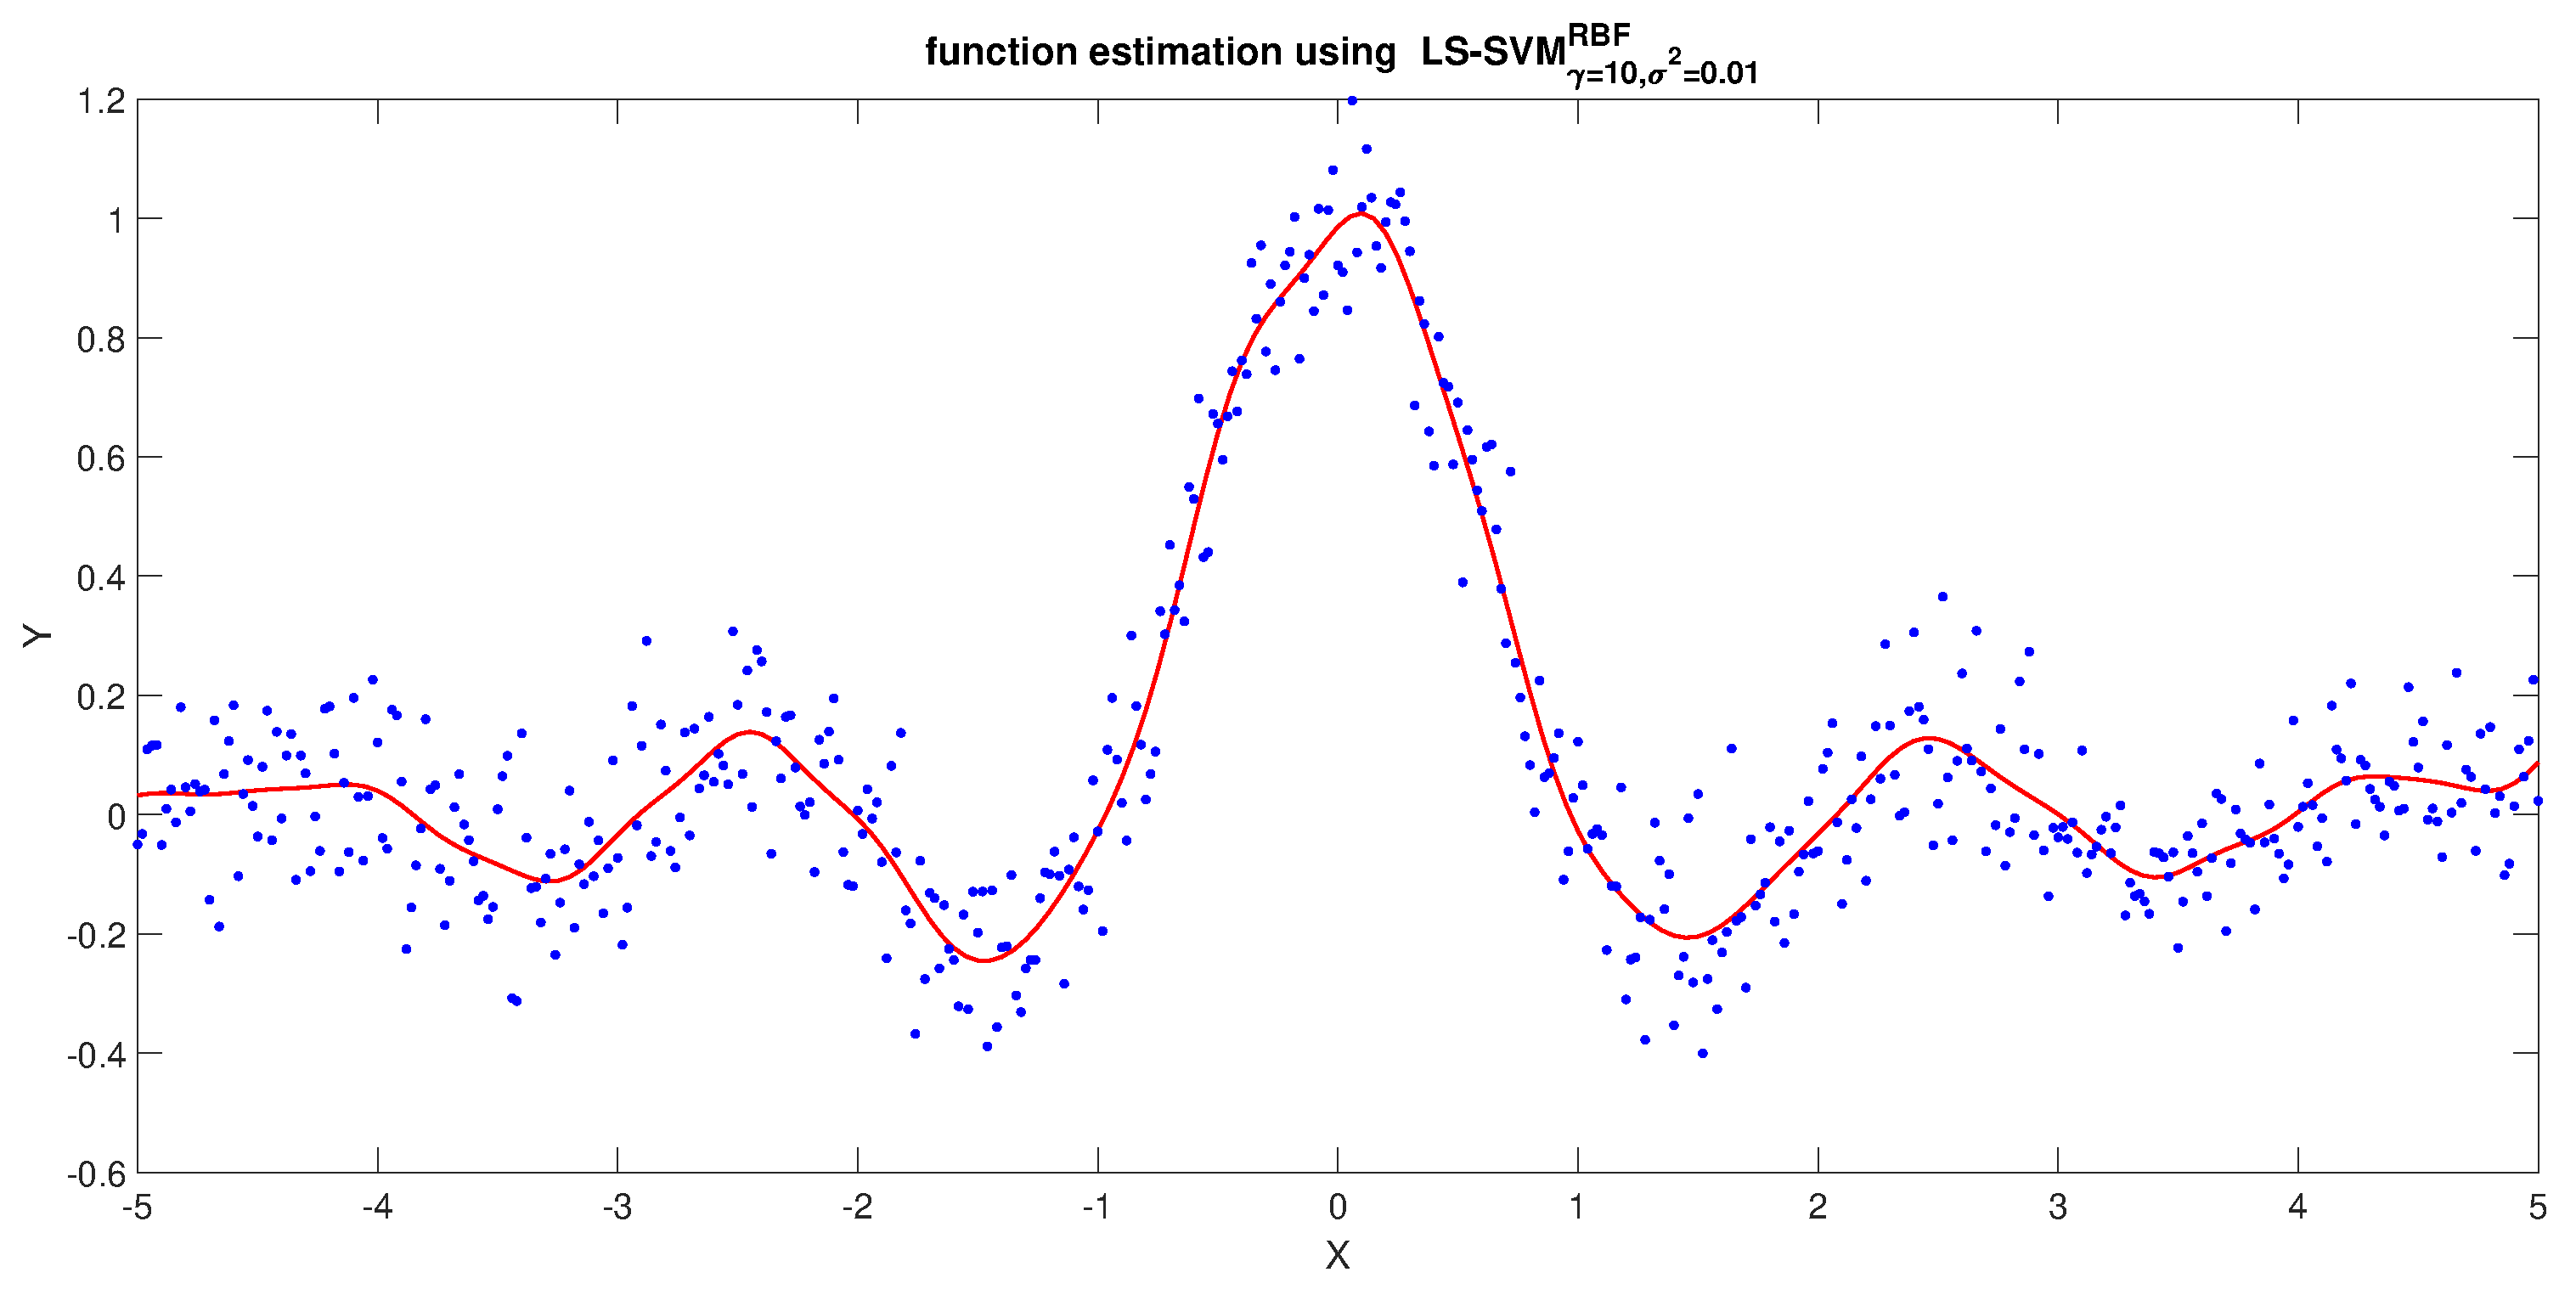
\includegraphics[width = 0.85\textwidth]{Exercise2/Report/Ex_1_2_1_gam(10)_sig(0.01)}
		\caption{$\gamma = 10$ ; $\sigma^2 = 0.01$}\label{fig:Ex_1_2_1_gam(10)_sig(0.01)}
	\end{subfigure}%
	\begin{subfigure}[b]{0.35\textwidth}
		\centering
		\captionsetup{width=0.8\linewidth}
		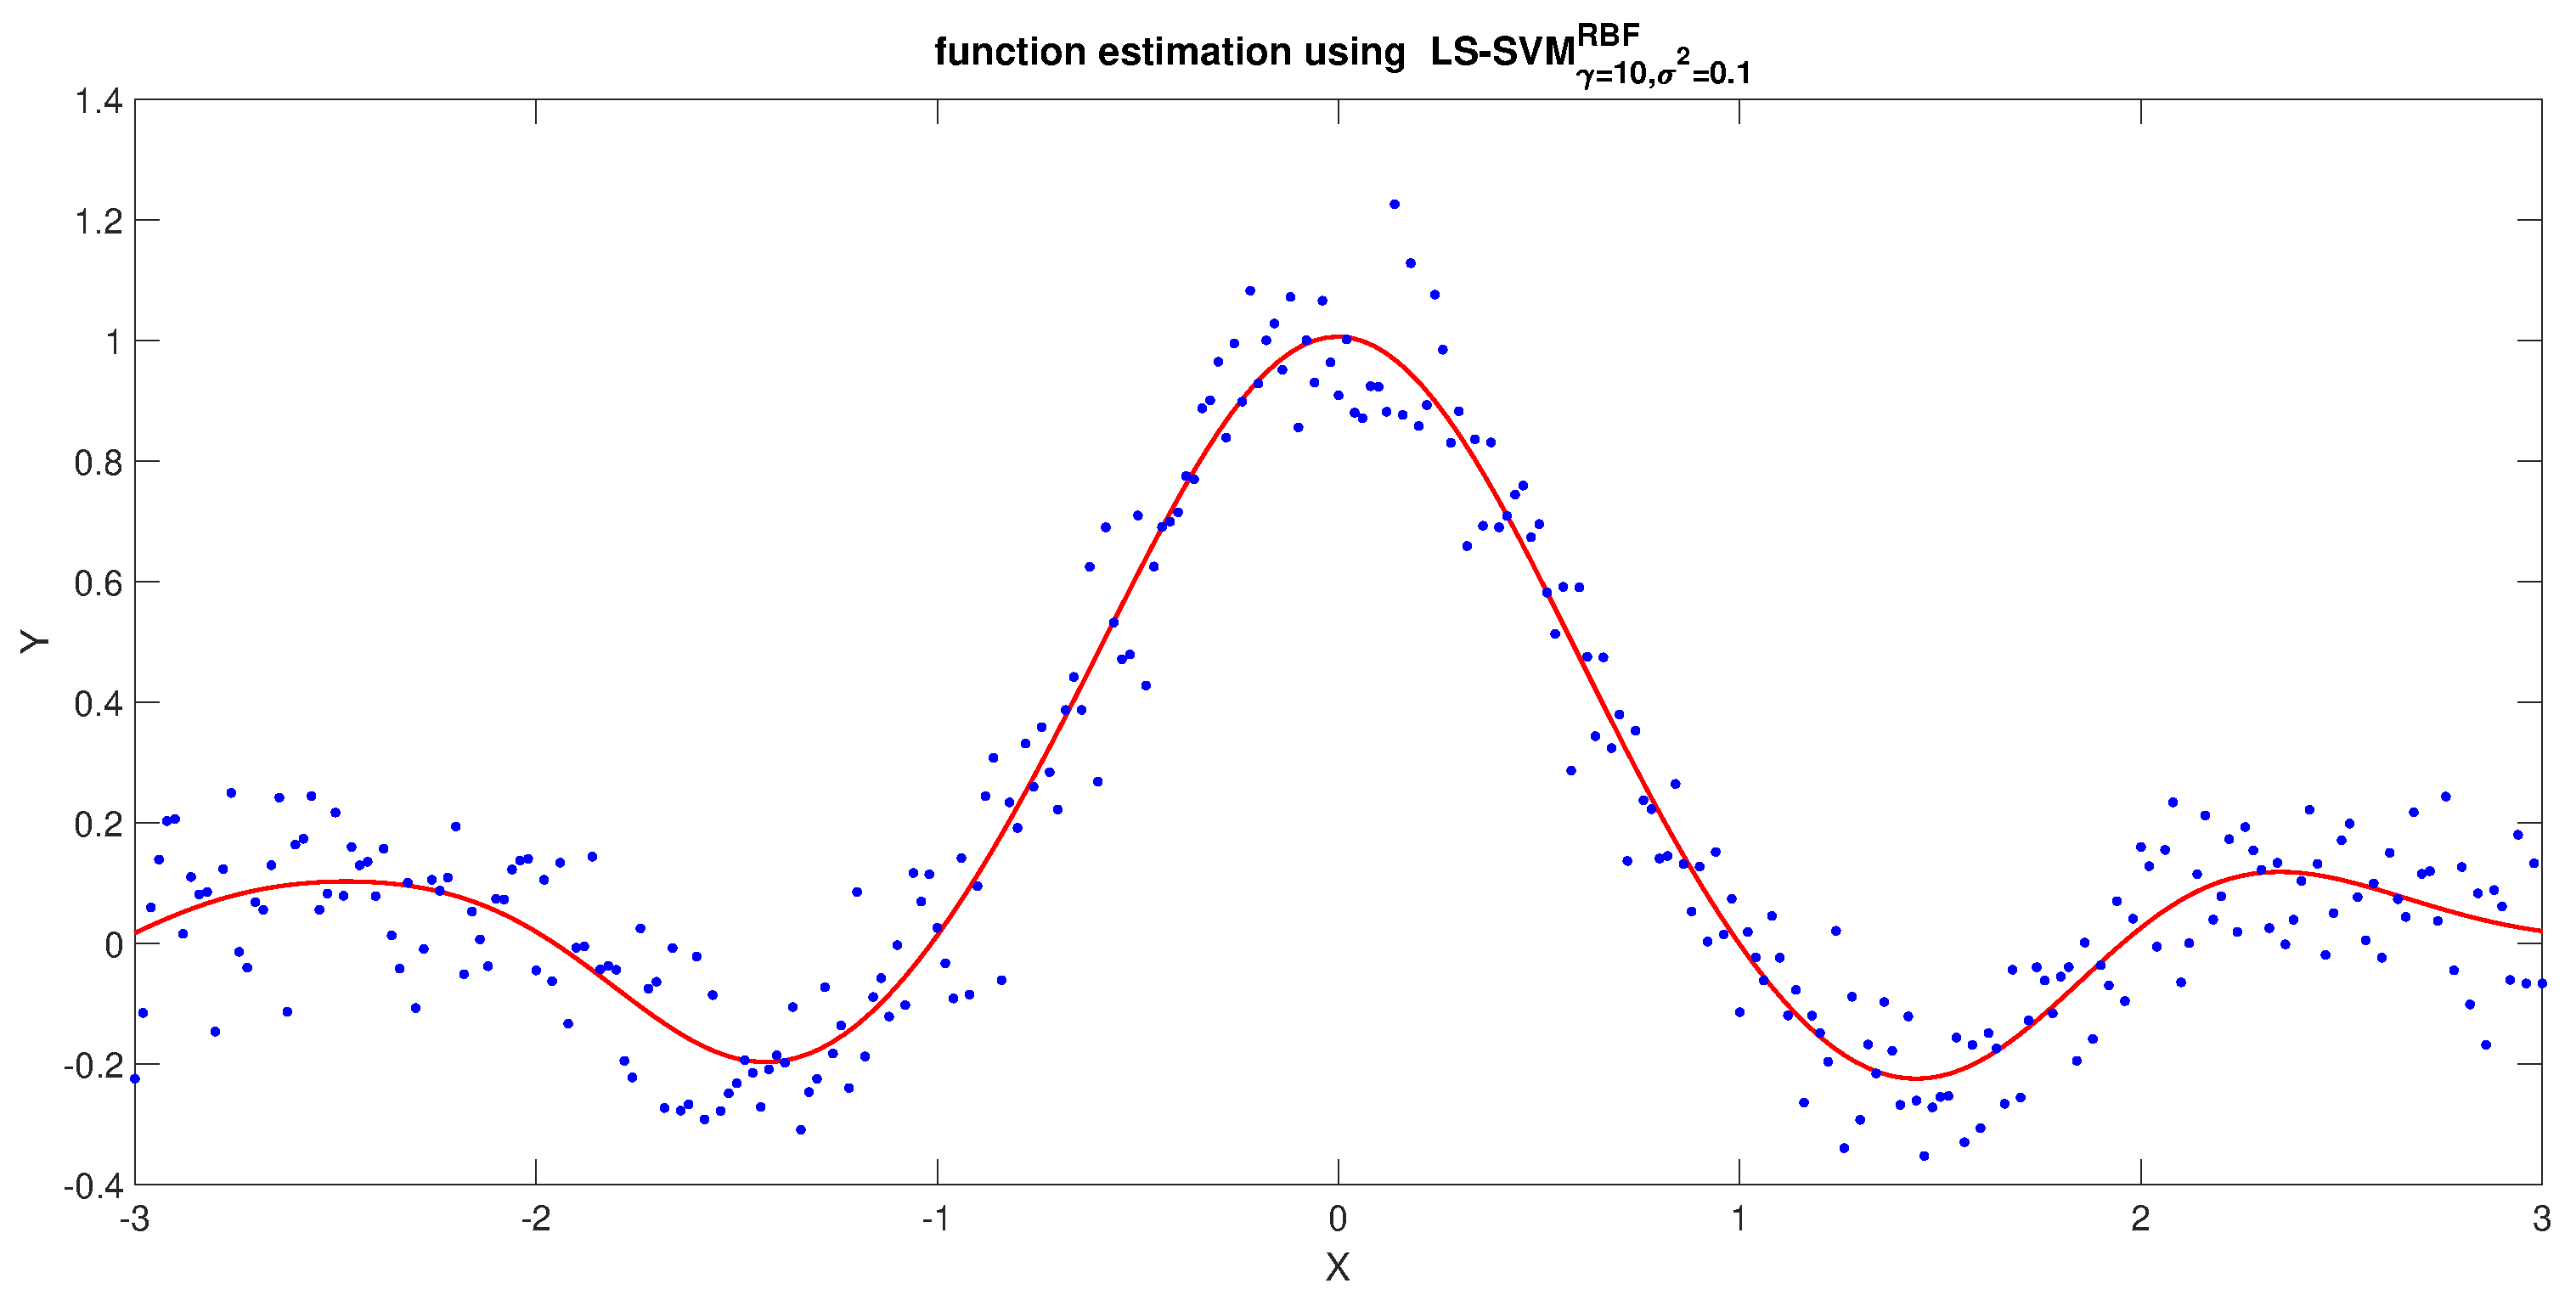
\includegraphics[width = 0.85\textwidth]{Exercise2/Report/Ex_1_2_1_gam(10)_sig(0.1)}
		\caption{$\gamma = 10$ ; $\sigma^2 = 0.1$}\label{fig:Ex_1_2_1_gam(10)_sig(0.1)}
	\end{subfigure}%
	\begin{subfigure}[b]{0.35\textwidth}
		\centering
		\captionsetup{width=0.8\linewidth}
		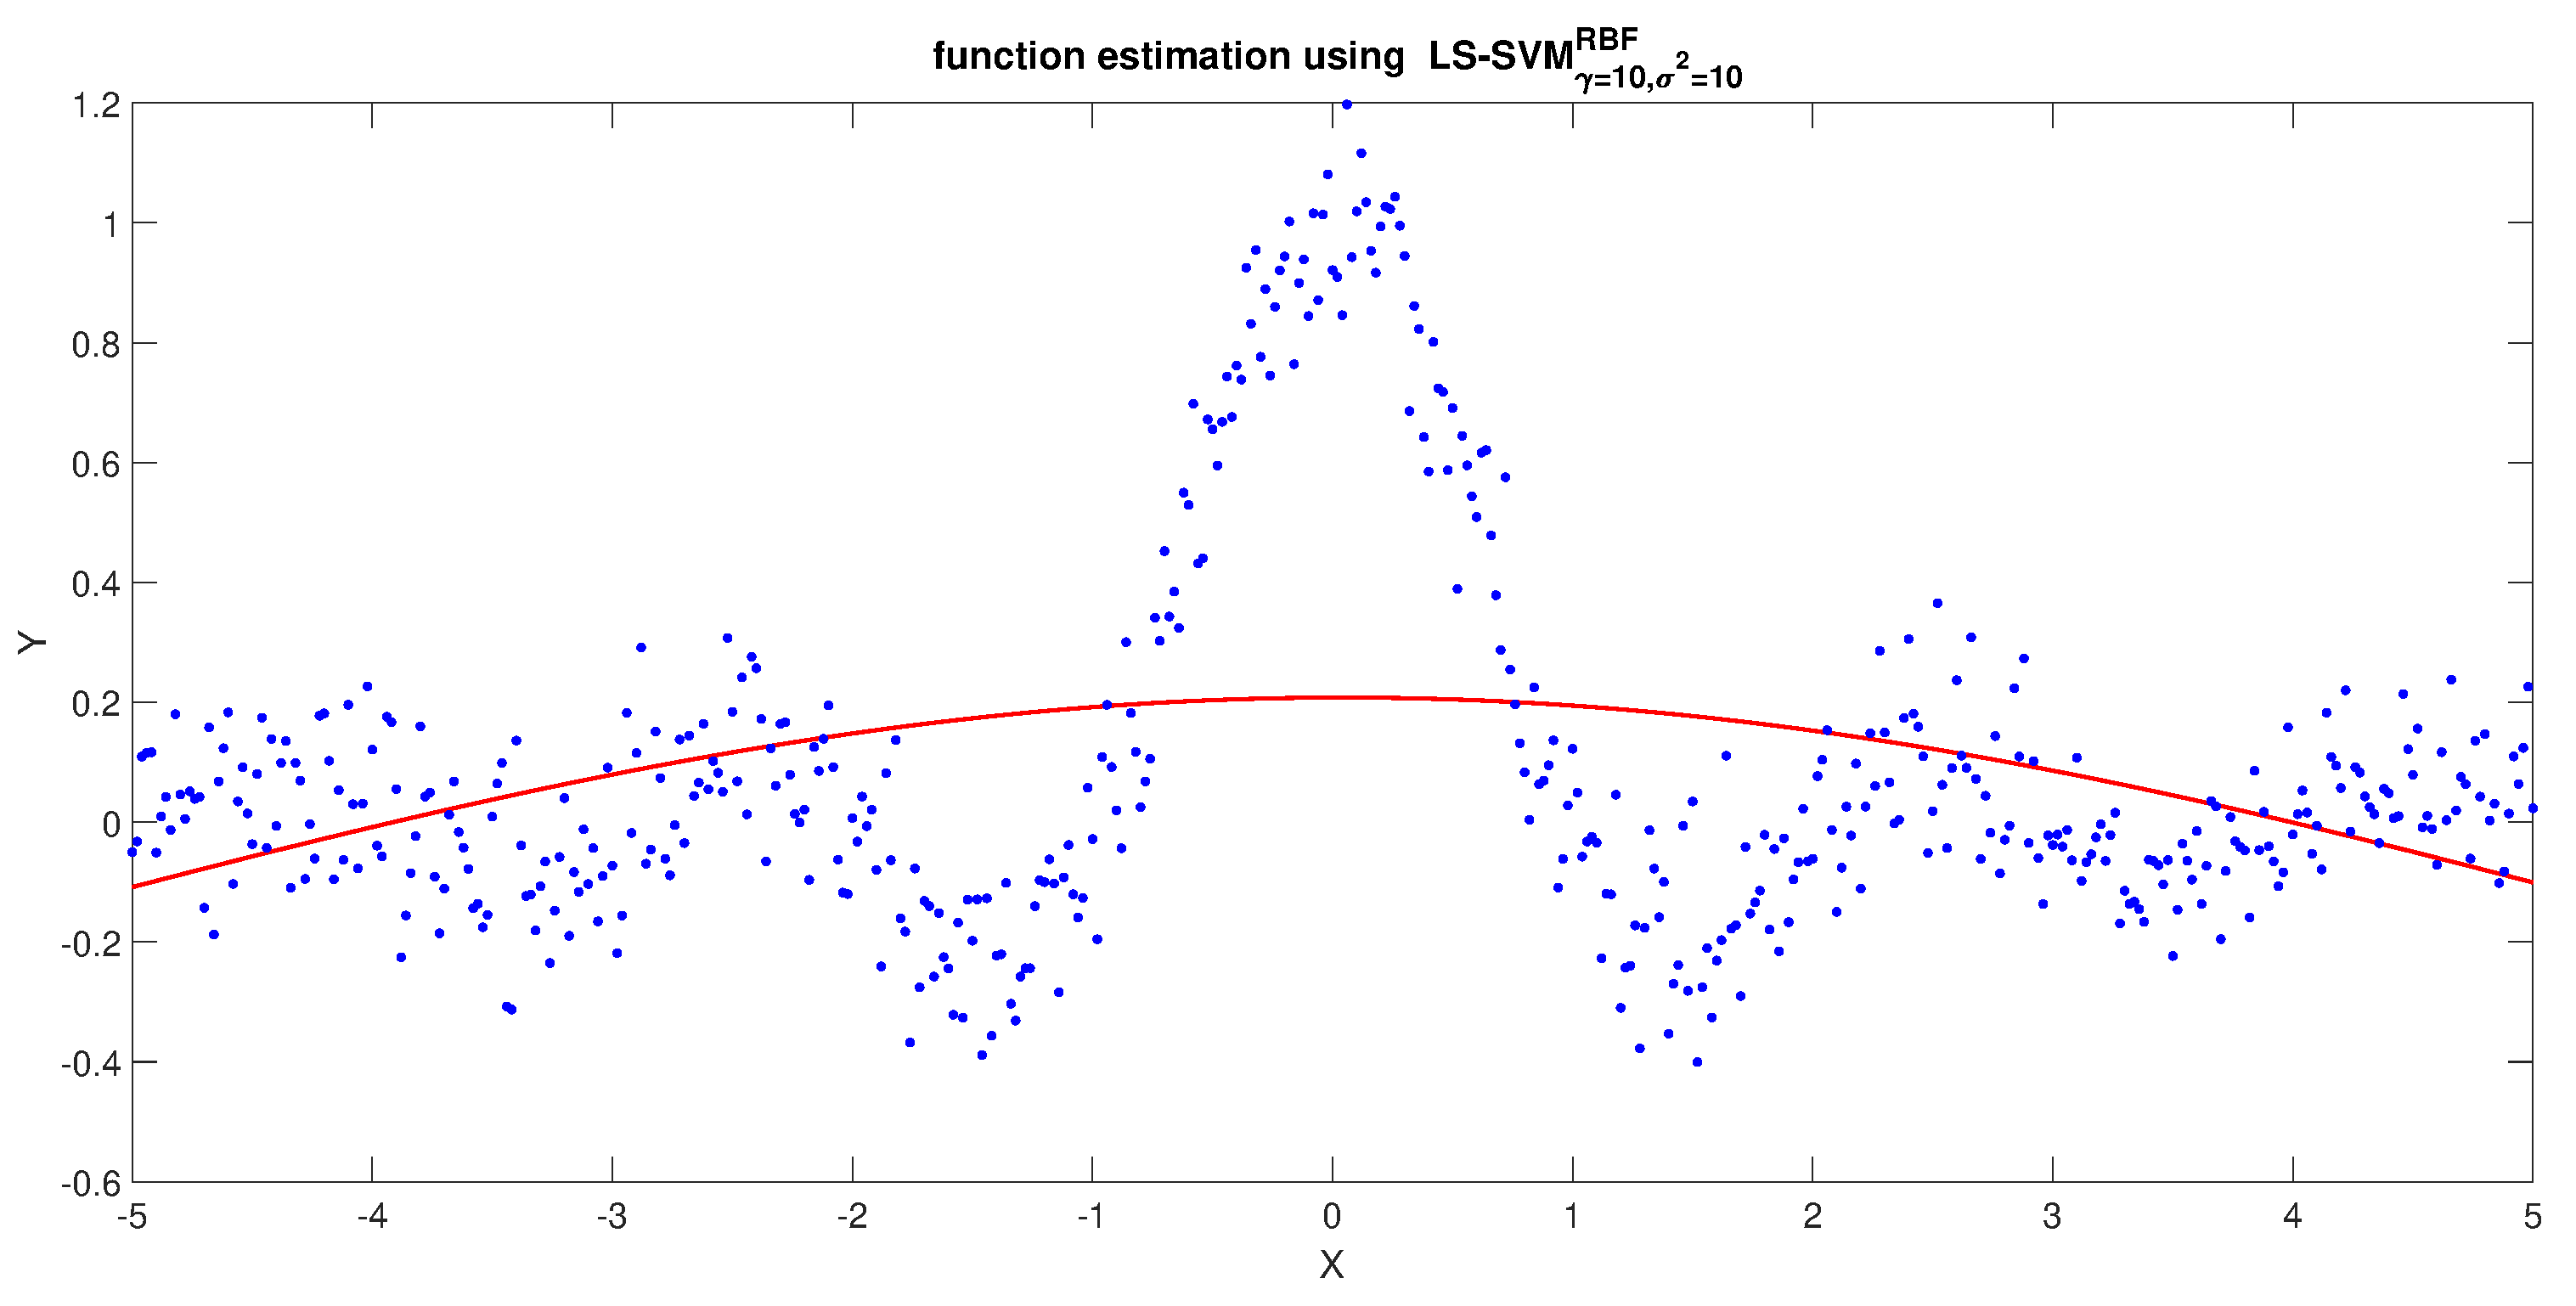
\includegraphics[width = 0.85\textwidth]{Exercise2/Report/Ex_1_2_1_gam(10)_sig(10)}
		\caption{$\gamma = 10$ ; $\sigma^2 = 10$}\label{fig:Ex_1_2_1_gam(10)_sig(10)}
	\end{subfigure}
	\begin{subfigure}[b]{0.35\textwidth}
		\centering
		\captionsetup{width=0.8\linewidth}
		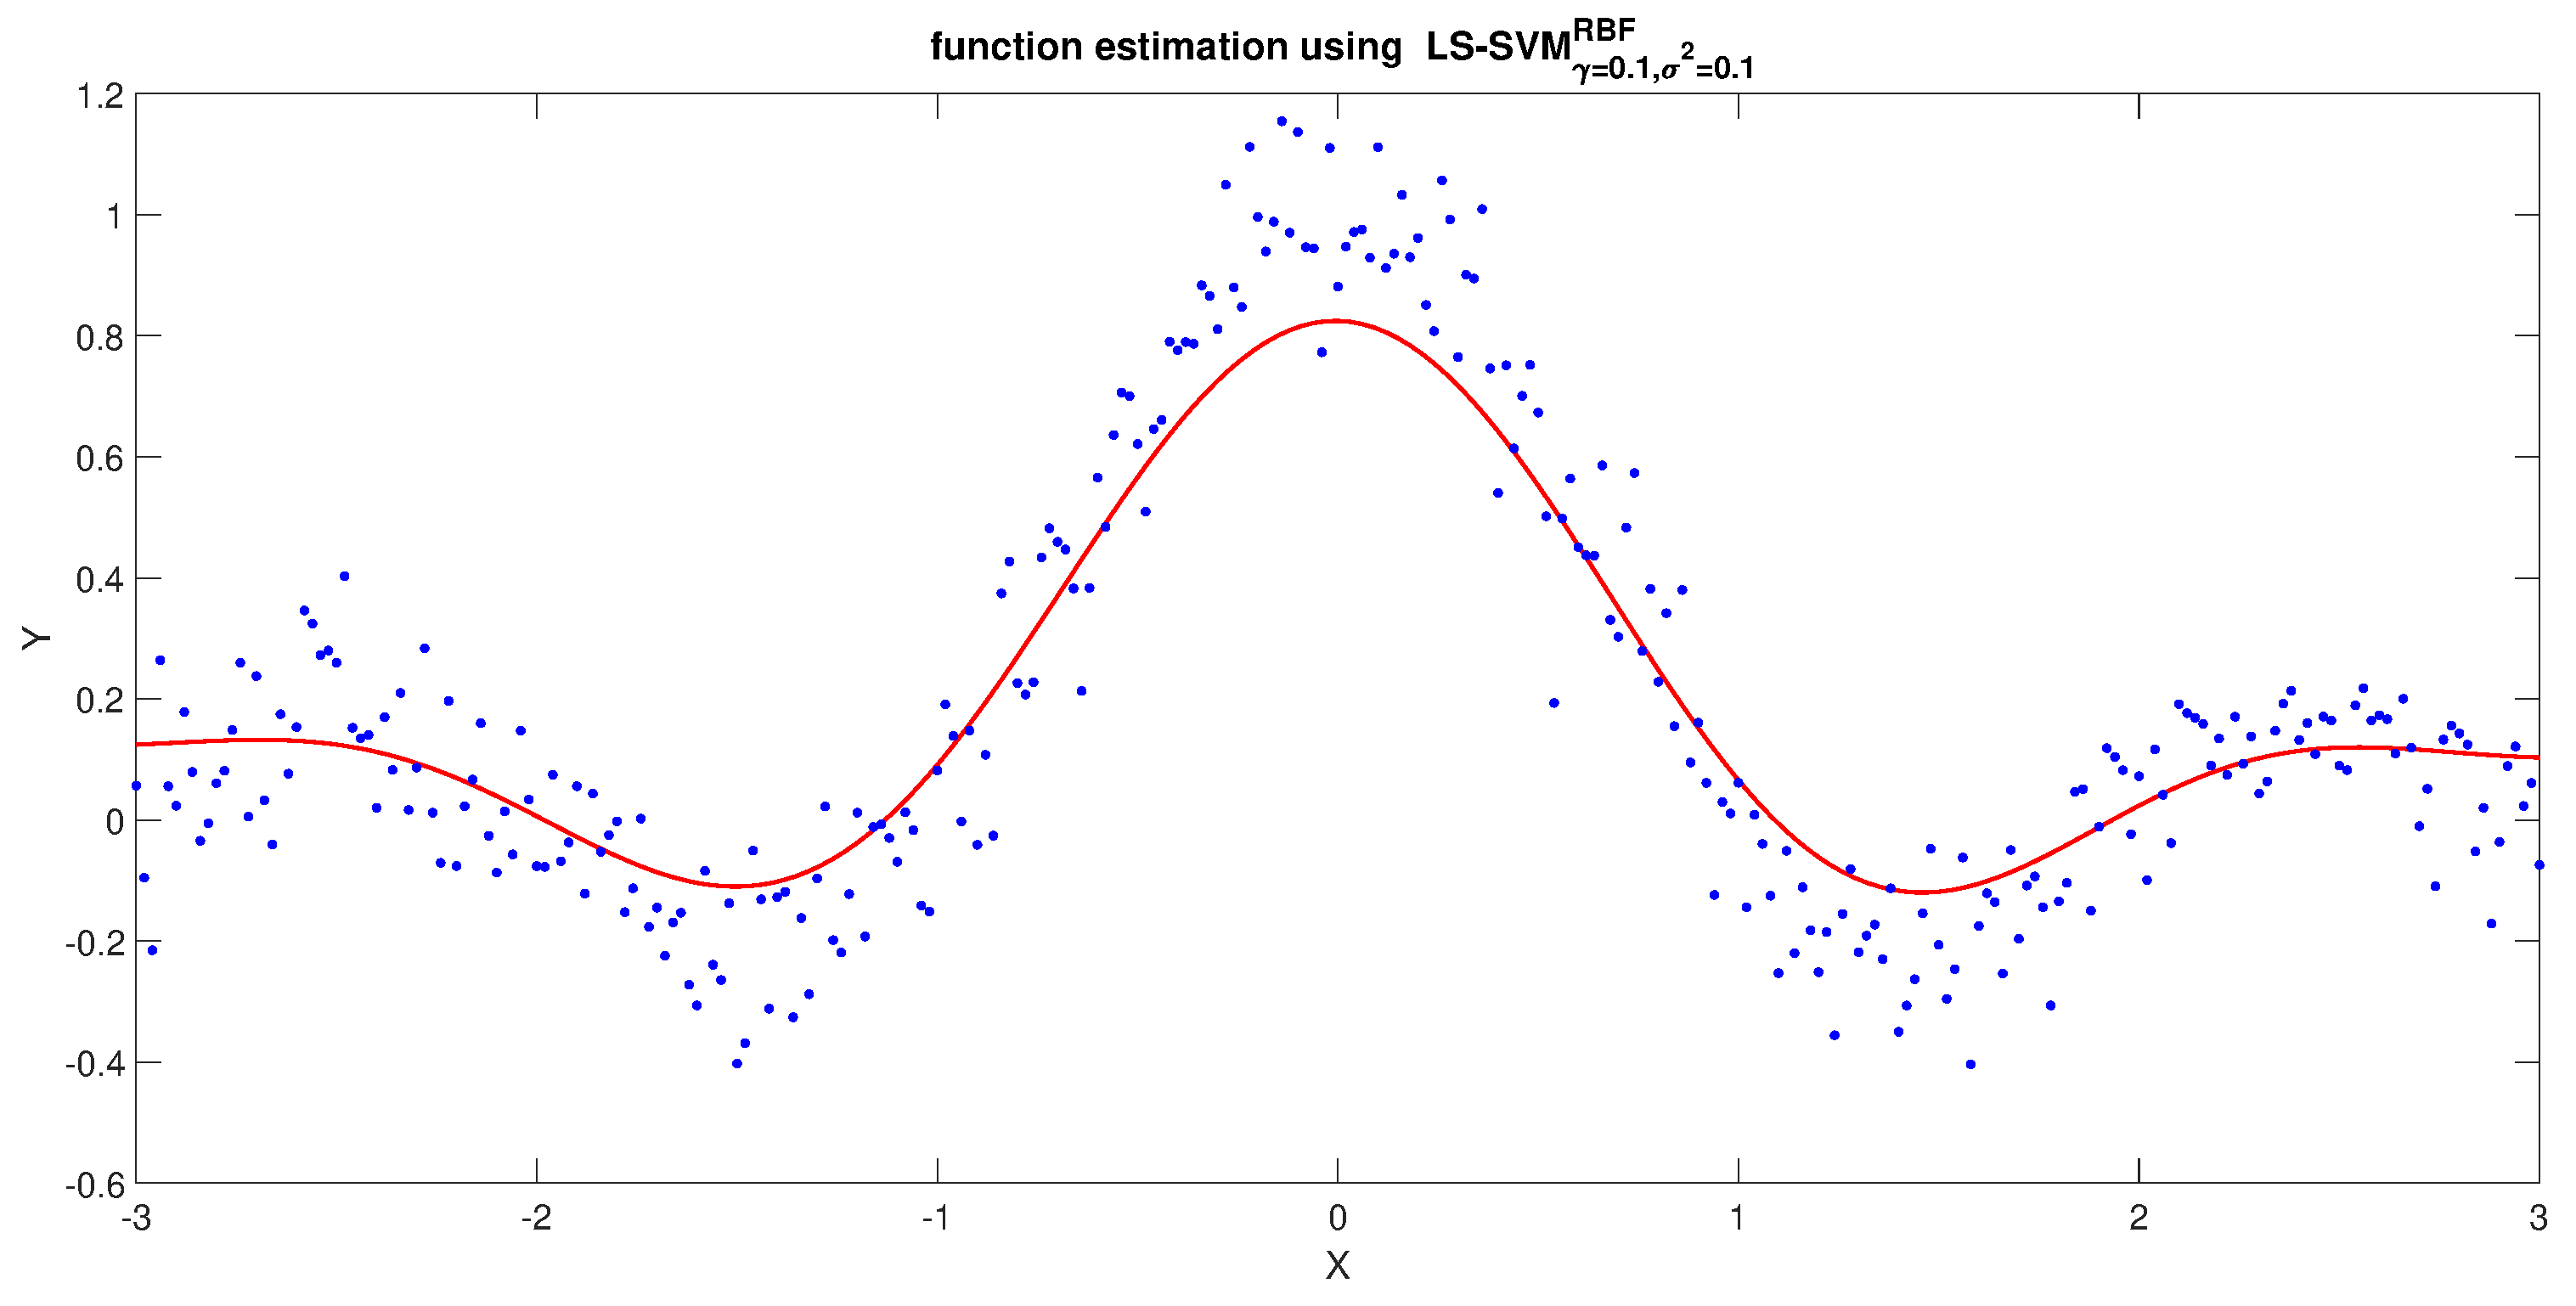
\includegraphics[width = 0.85\textwidth]{Exercise2/Report/Ex_1_2_1_gam(0.1)_sig(0.1)}
		\caption{$\gamma = 0.1$ ; $\sigma^2 = 0.1$}\label{fig:Ex_1_2_1_gam(0.1)_sig(0.1)}
	\end{subfigure}%
	\begin{subfigure}[b]{0.35\textwidth}
		\centering
		\captionsetup{width=0.8\linewidth}
		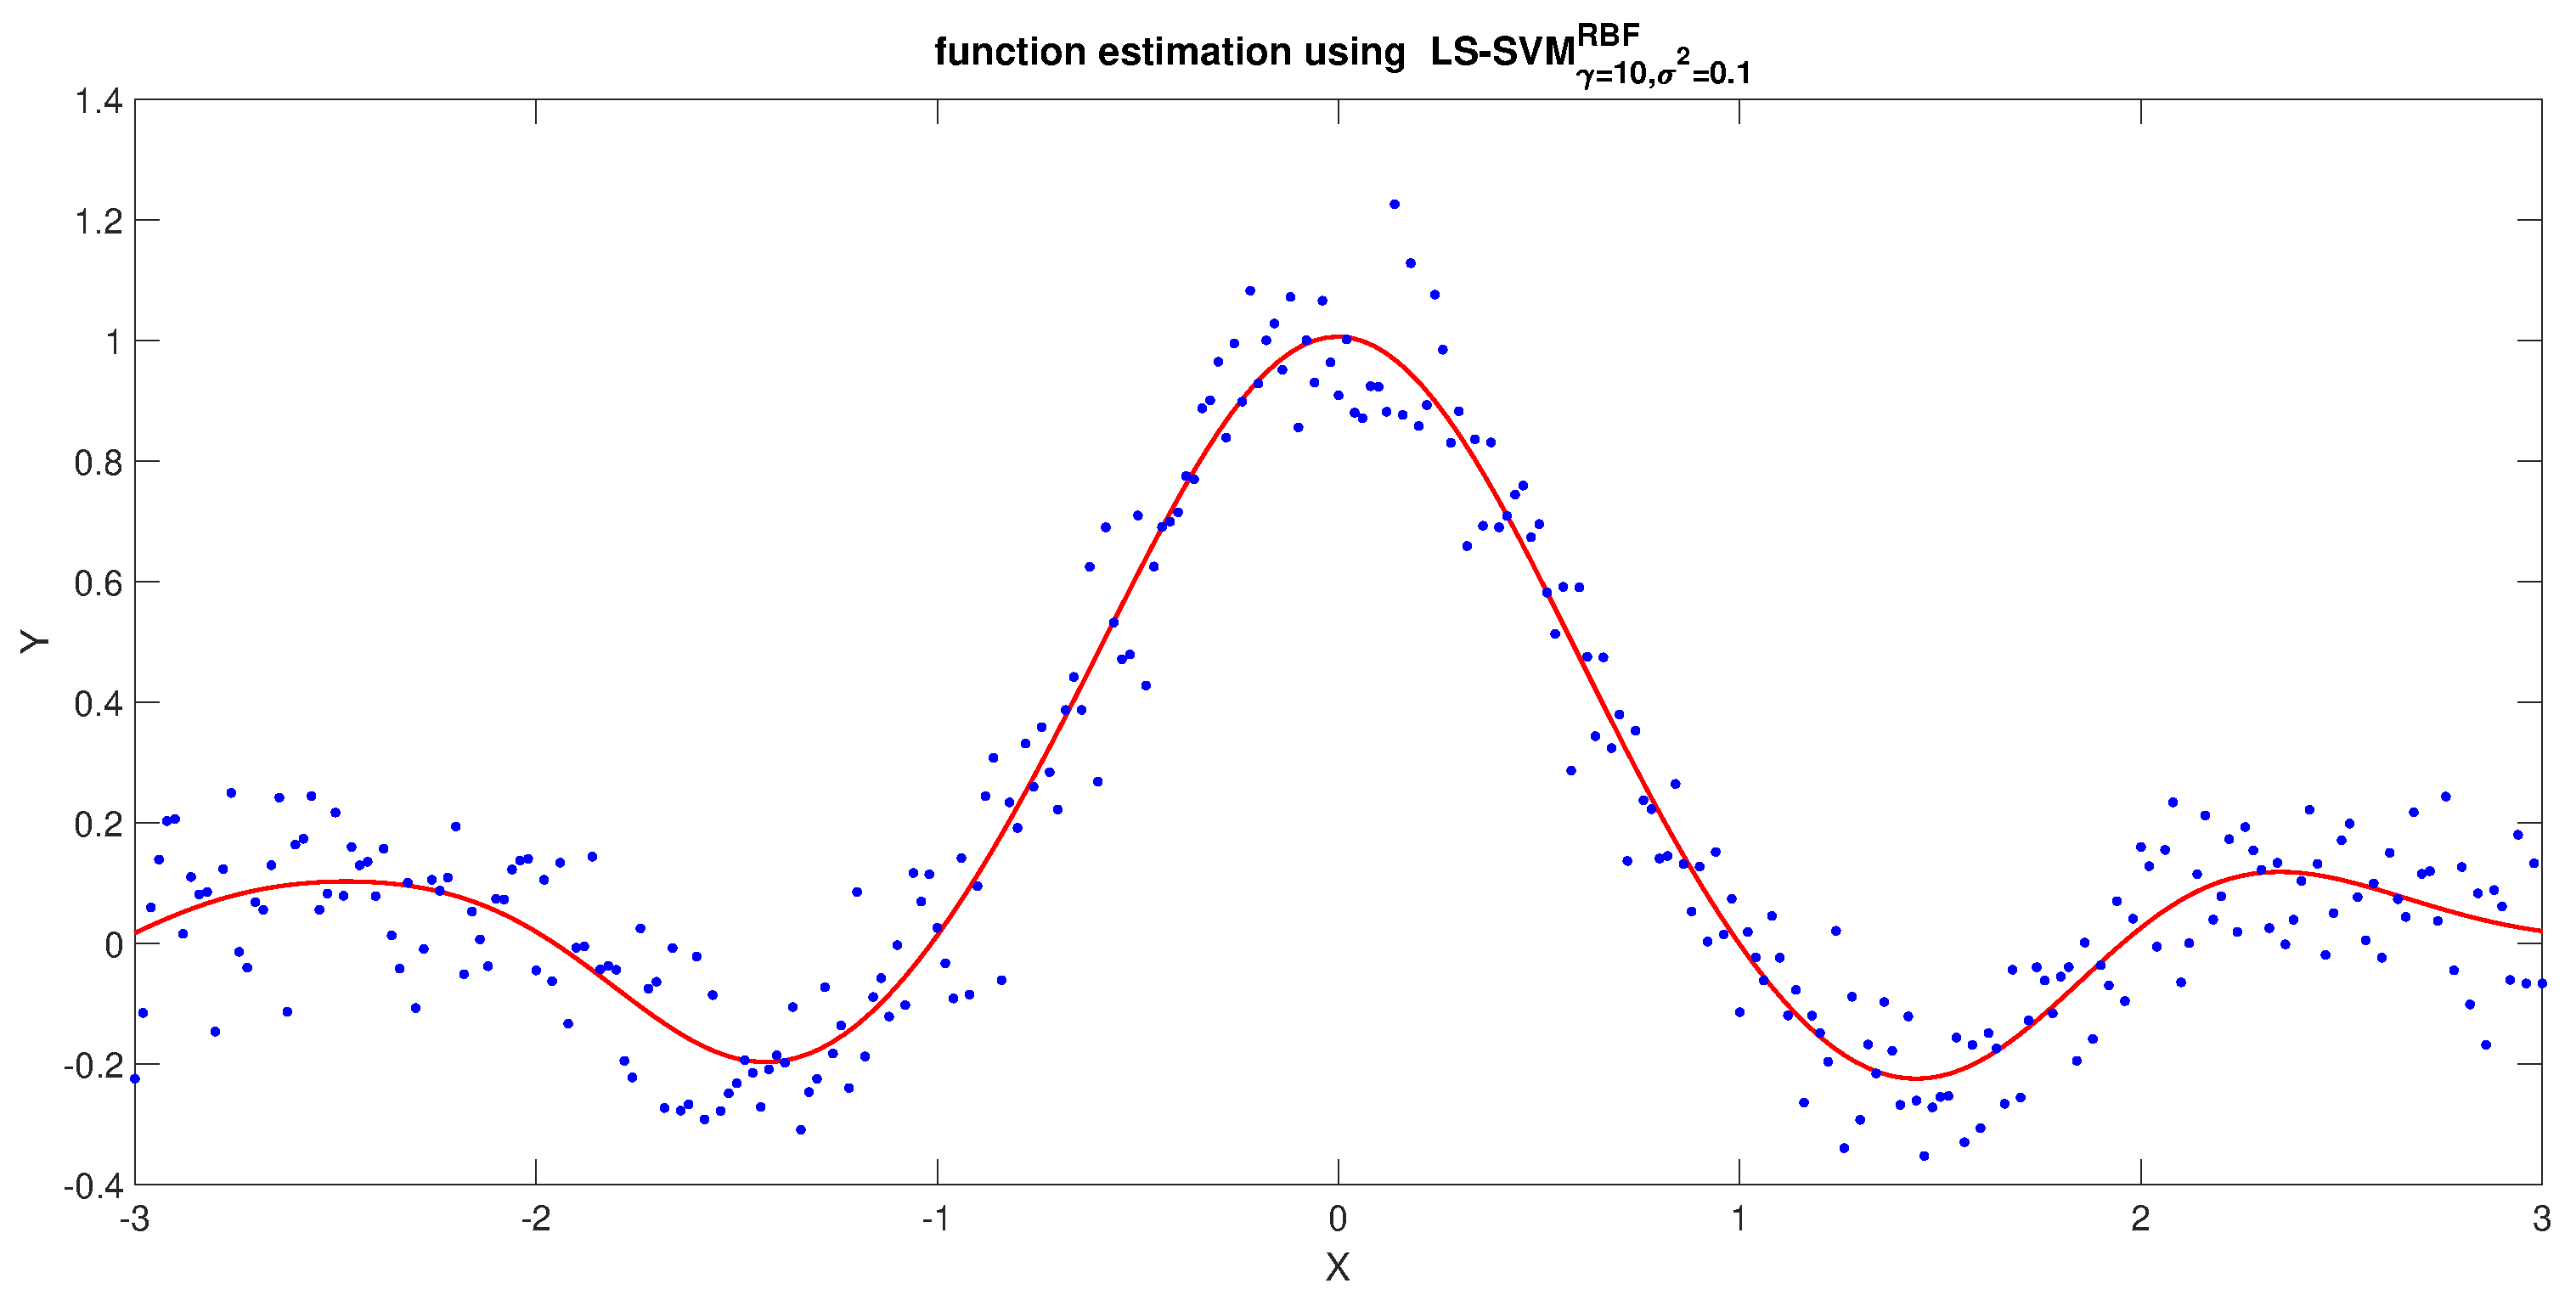
\includegraphics[width = 0.85\textwidth]{Exercise2/Report/Ex_1_2_1_gam(10)_sig(0.1)}
		\caption{$\gamma = 10$ ; $\sigma^2 = 0.1$ }\label{fig:Ex_1_2_1_gam(1)_sig(0.1)}
	\end{subfigure}%
	\begin{subfigure}[b]{0.35\textwidth}
		\centering
		\captionsetup{width=0.8\linewidth}
		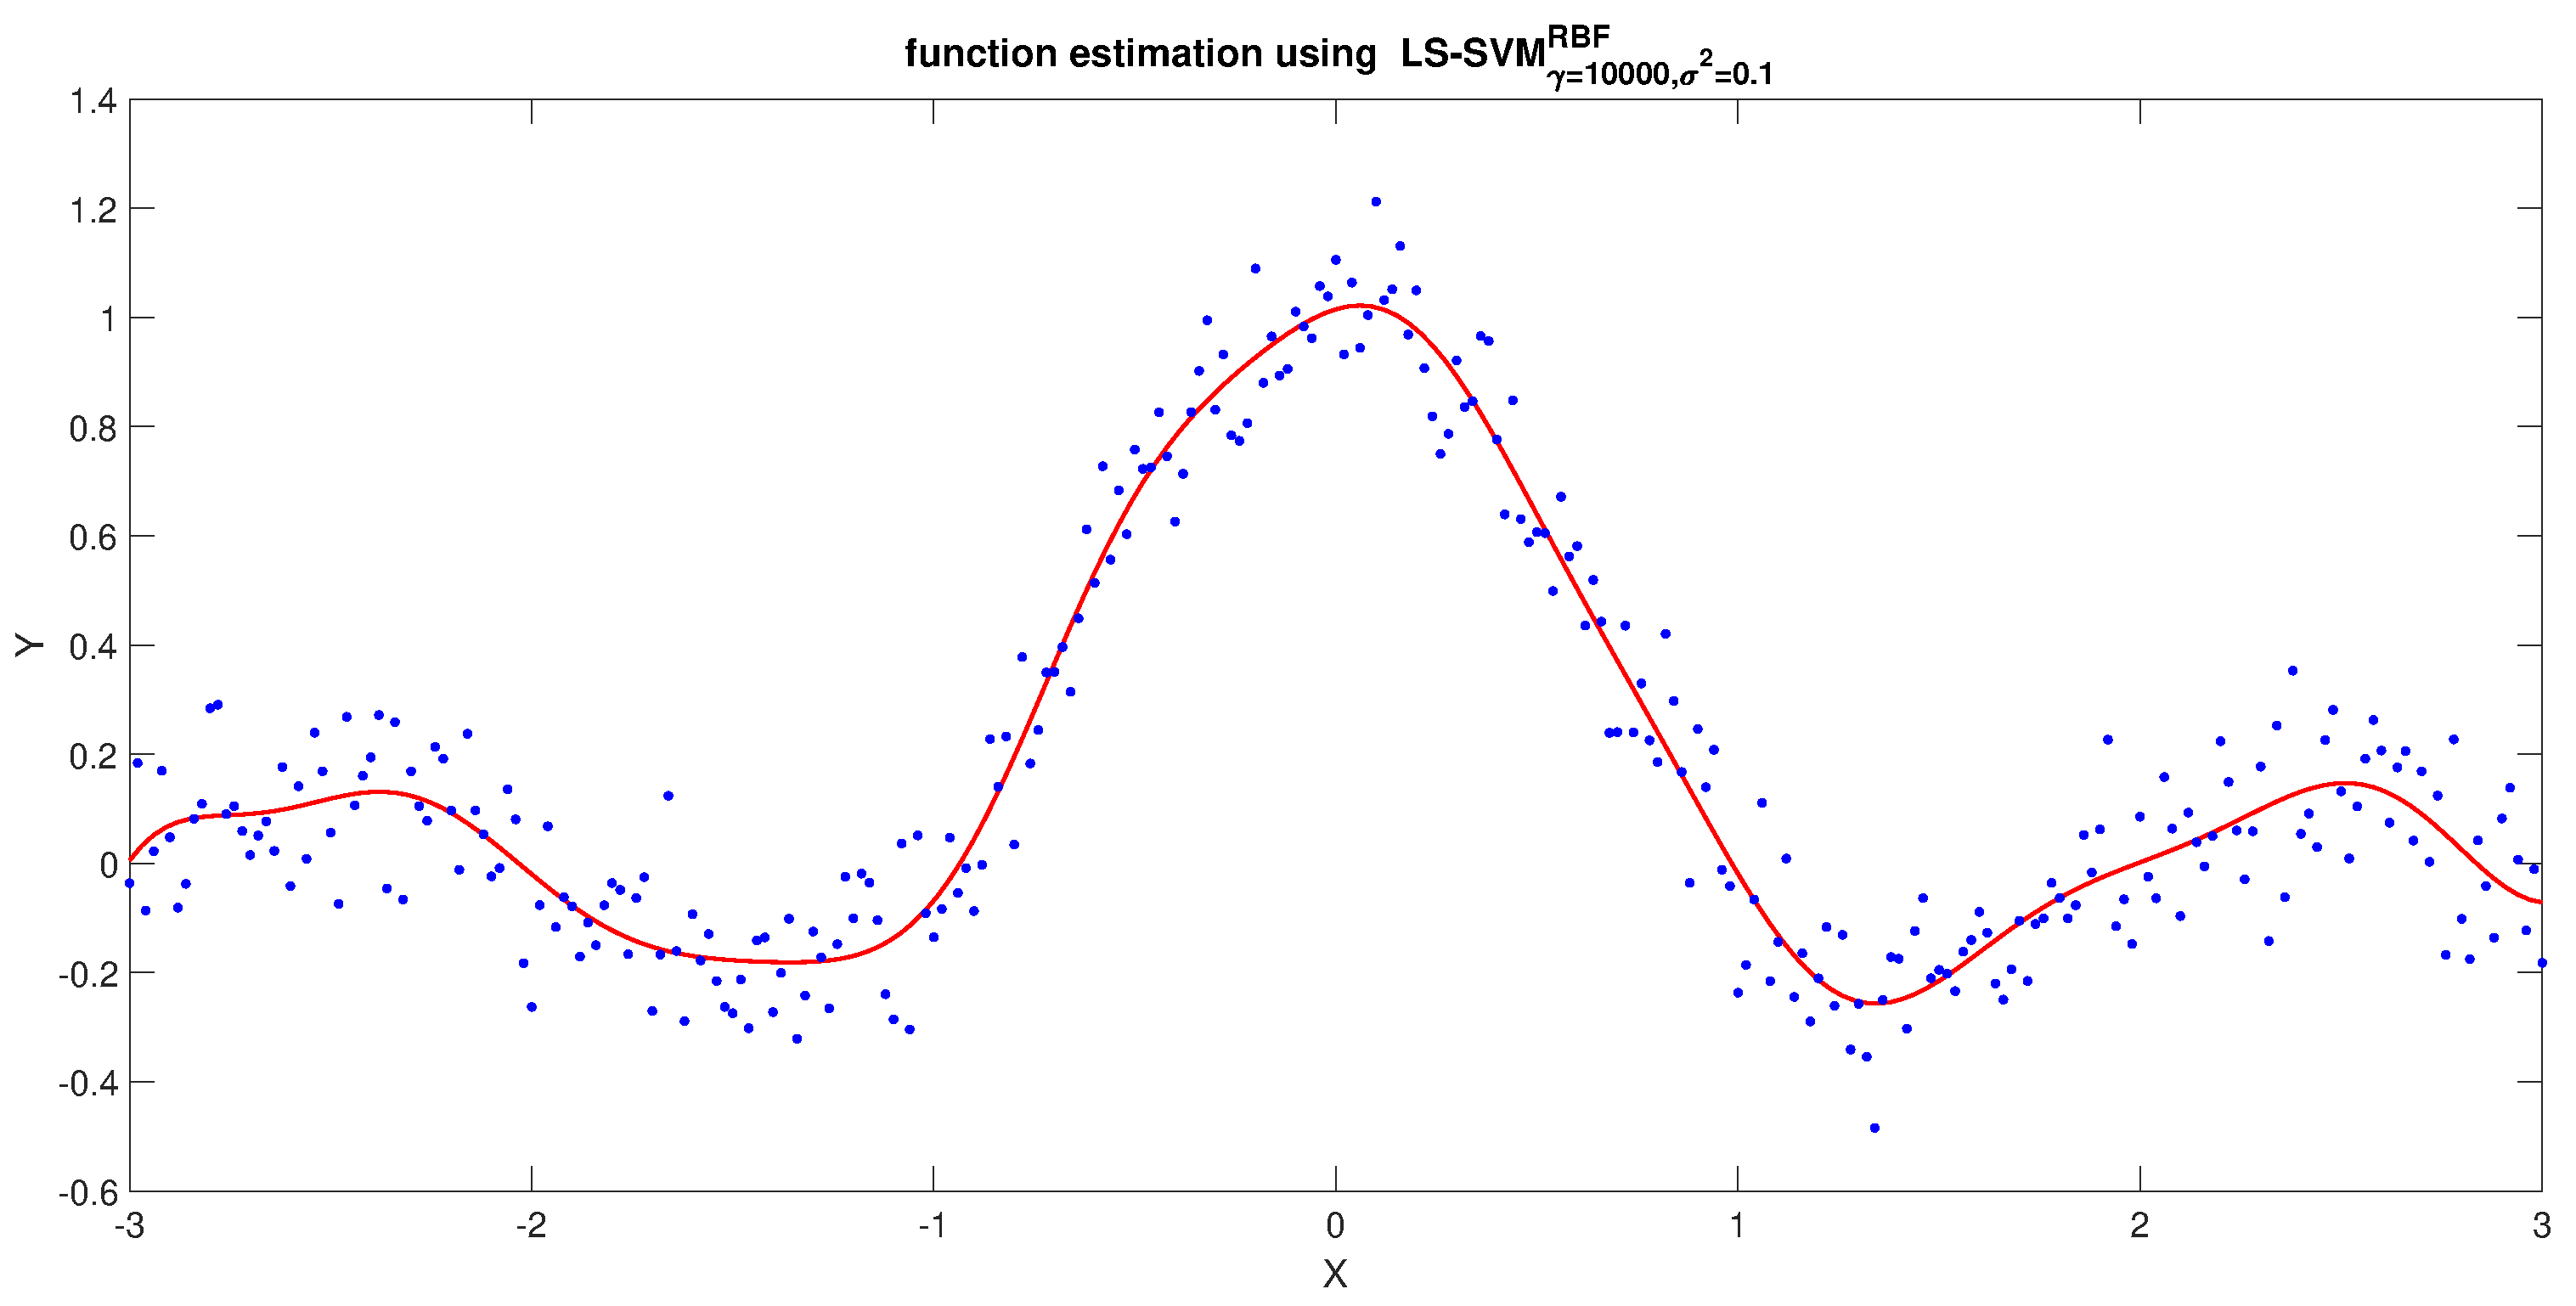
\includegraphics[width = 0.85\textwidth]{Exercise2/Report/Ex_1_2_1_gam(10000)_sig(0.1)}
		\caption{$\gamma = 10000$ ; $\sigma^2 = 0.1$}\label{fig:Ex_1_2_1_gam(10000)_sig(0.1)}
	\end{subfigure}
	\caption{SVM Regressor : Function estimation for various ($\gamma$; $\sigma^2$) values of the RBF kernel}
	\label{fig:sinc_regress}
\end{figure}
\begin{table}[!htpb]
	\centering
	\begin{tabular}{ ||p{1.8cm}||p{1.8cm}|p{1.8cm}|p{1.8cm}|p{1.8cm}|p{1.8cm}|p{1.8cm}|}
		\hline
		\multicolumn{7}{|c|}{Mean Squared Error (MSE) (\%)} \\ \hline\hline
		\cellcolor{blue!25}($\gamma$ ; $\sigma^2$) &\cellcolor{blue!25}$\sigma^2 = 0.01$ & \cellcolor{blue!25}$\sigma^2 = 0.1$ &\cellcolor{blue!25}$\sigma^2 = 1$ & \cellcolor{blue!25}$\sigma^2 = 10$ &\cellcolor{blue!25}$\sigma^2 = 10^2$ &\cellcolor{blue!25}$\sigma^2 = 10^3$ \\ \hline \hline
		\cellcolor{blue!25}$\gamma = 0.1$ &2.2498&1.5692&8.3871&12.988&13.631&13.641 \\ \hline
		\cellcolor{blue!25}$\gamma = 1$ &1.1784&1.1024&5.1397&11.392&13.553&13.639 \\ \hline
		\cellcolor{blue!25}$\gamma = 10$ &1.2326&1.121&3.261&10.967&12.937&13.631 \\ \hline
		\cellcolor{blue!25}$\gamma = 10^2$ &1.2621&1.1367&1.481&10.526&11.474&13.552 \\ \hline
		\cellcolor{blue!25}$\gamma = 10^3$ &1.2758&1.1503&1.2254&8.2999&11.205&12.932 \\ \hline
		\cellcolor{blue!25}$\gamma = 10^4$ &1.2791&1.1612&1.1065&6.659&11.201&11.483 \\ \hline
	\end{tabular}
	\caption{MSE (\%) between SVR estimations and ground truth data for various ($\gamma$ ; $\sigma^2$)}
	\label{table:9}
\end{table}\\
\textbf{Do you think there is one optimal pair of hyperparameters? }

As seen from figure \ref{fig:sinc_regress} and table \ref{table:9}, it can be inferred that the model performs better and have least MSE for lower values of $\sigma^2$ such as 0.01 and 0.1 for $\gamma$ in range of 1 to $10^4)$.  One such optimal pair can be  ($\gamma$, $\sigma^2$) = (1 ; 0.1) and (10;0.1)\\
\newline
\textbf{Tune the gam and sig2 parameters using the tunelssvm procedure. Use multiple runs:
	what can you say about the hyperparameters and the results? Use both the simplex
	and gridsearch algorithms and report differences.}

\begin{wraptable}[11]{l}{.7\textwidth}
	\centering
	\begin{tabular}{ |p{1.5cm}|p{1.5cm}|p{1.7cm}||p{1.5cm}|p{1.5cm}|p{1.7cm}| }
		\hline
		\multicolumn{3}{|c||}{Simplex Algorithm} &\multicolumn{3}{c|}{Grid Search Algorithm}
		\\ \hline	
		\cellcolor{blue!25}$\gamma$ &\cellcolor{blue!25}$\sigma^2$ & \cellcolor{blue!25}cost & \cellcolor{blue!25}$\gamma$ &\cellcolor{blue!25}$\sigma^2$ &\cellcolor{blue!25}cost \\ \hline
		44.681 &0.36072 &0.0099951 &222.33 &0.44703 &0.0098997 \\ \hline
		390.57 &0.48974 &0.010855 &21.733  &0.33129 &0.010041 \\ \hline
		46.424 &0.38045 &0.010003 &44.117  &0.3663   &0.0099097 \\ \hline
		76.299 & 0.39569 &0.010843 &23.237  &0.34383  &0.0099472 \\ \hline
		57.125 &0.39352 &0.0099651 &16.346 &0.31191 &0.010876 \\ \hline
		
	\end{tabular}
	\caption{Optimal ($\gamma$, $\sigma^2$) pairs using auto tuning methods}
	\label{table:10}
\end{wraptable}
From table \ref{table:10} it can seen that both the algorithms produce different optimal ($\gamma$;$\sigma^2$) for each run but the error approximately remains the same. Also, a lot of variability is seen only in $\gamma$ values whereas $\sigma^2$ has much lesser variance. Overall, it can be said that $\gamma$ $>>$ $\sigma^2$. Also, simplex algorithm executes faster with 0.85 secs compared to grid search method which takes 1.2 sec approximately. 
\subsection{Application of the Bayesian framework}
\textbf{Discuss in a schematic way how parameter tuning works using the Bayesian framework.
	Illustrate this scheme by interpreting the function calls denoted above.}

\begin{figure}[ht]
	\centering
	\begin{subfigure}[b]{0.5\textwidth}
		\centering
		\captionsetup{width=0.7\linewidth}
		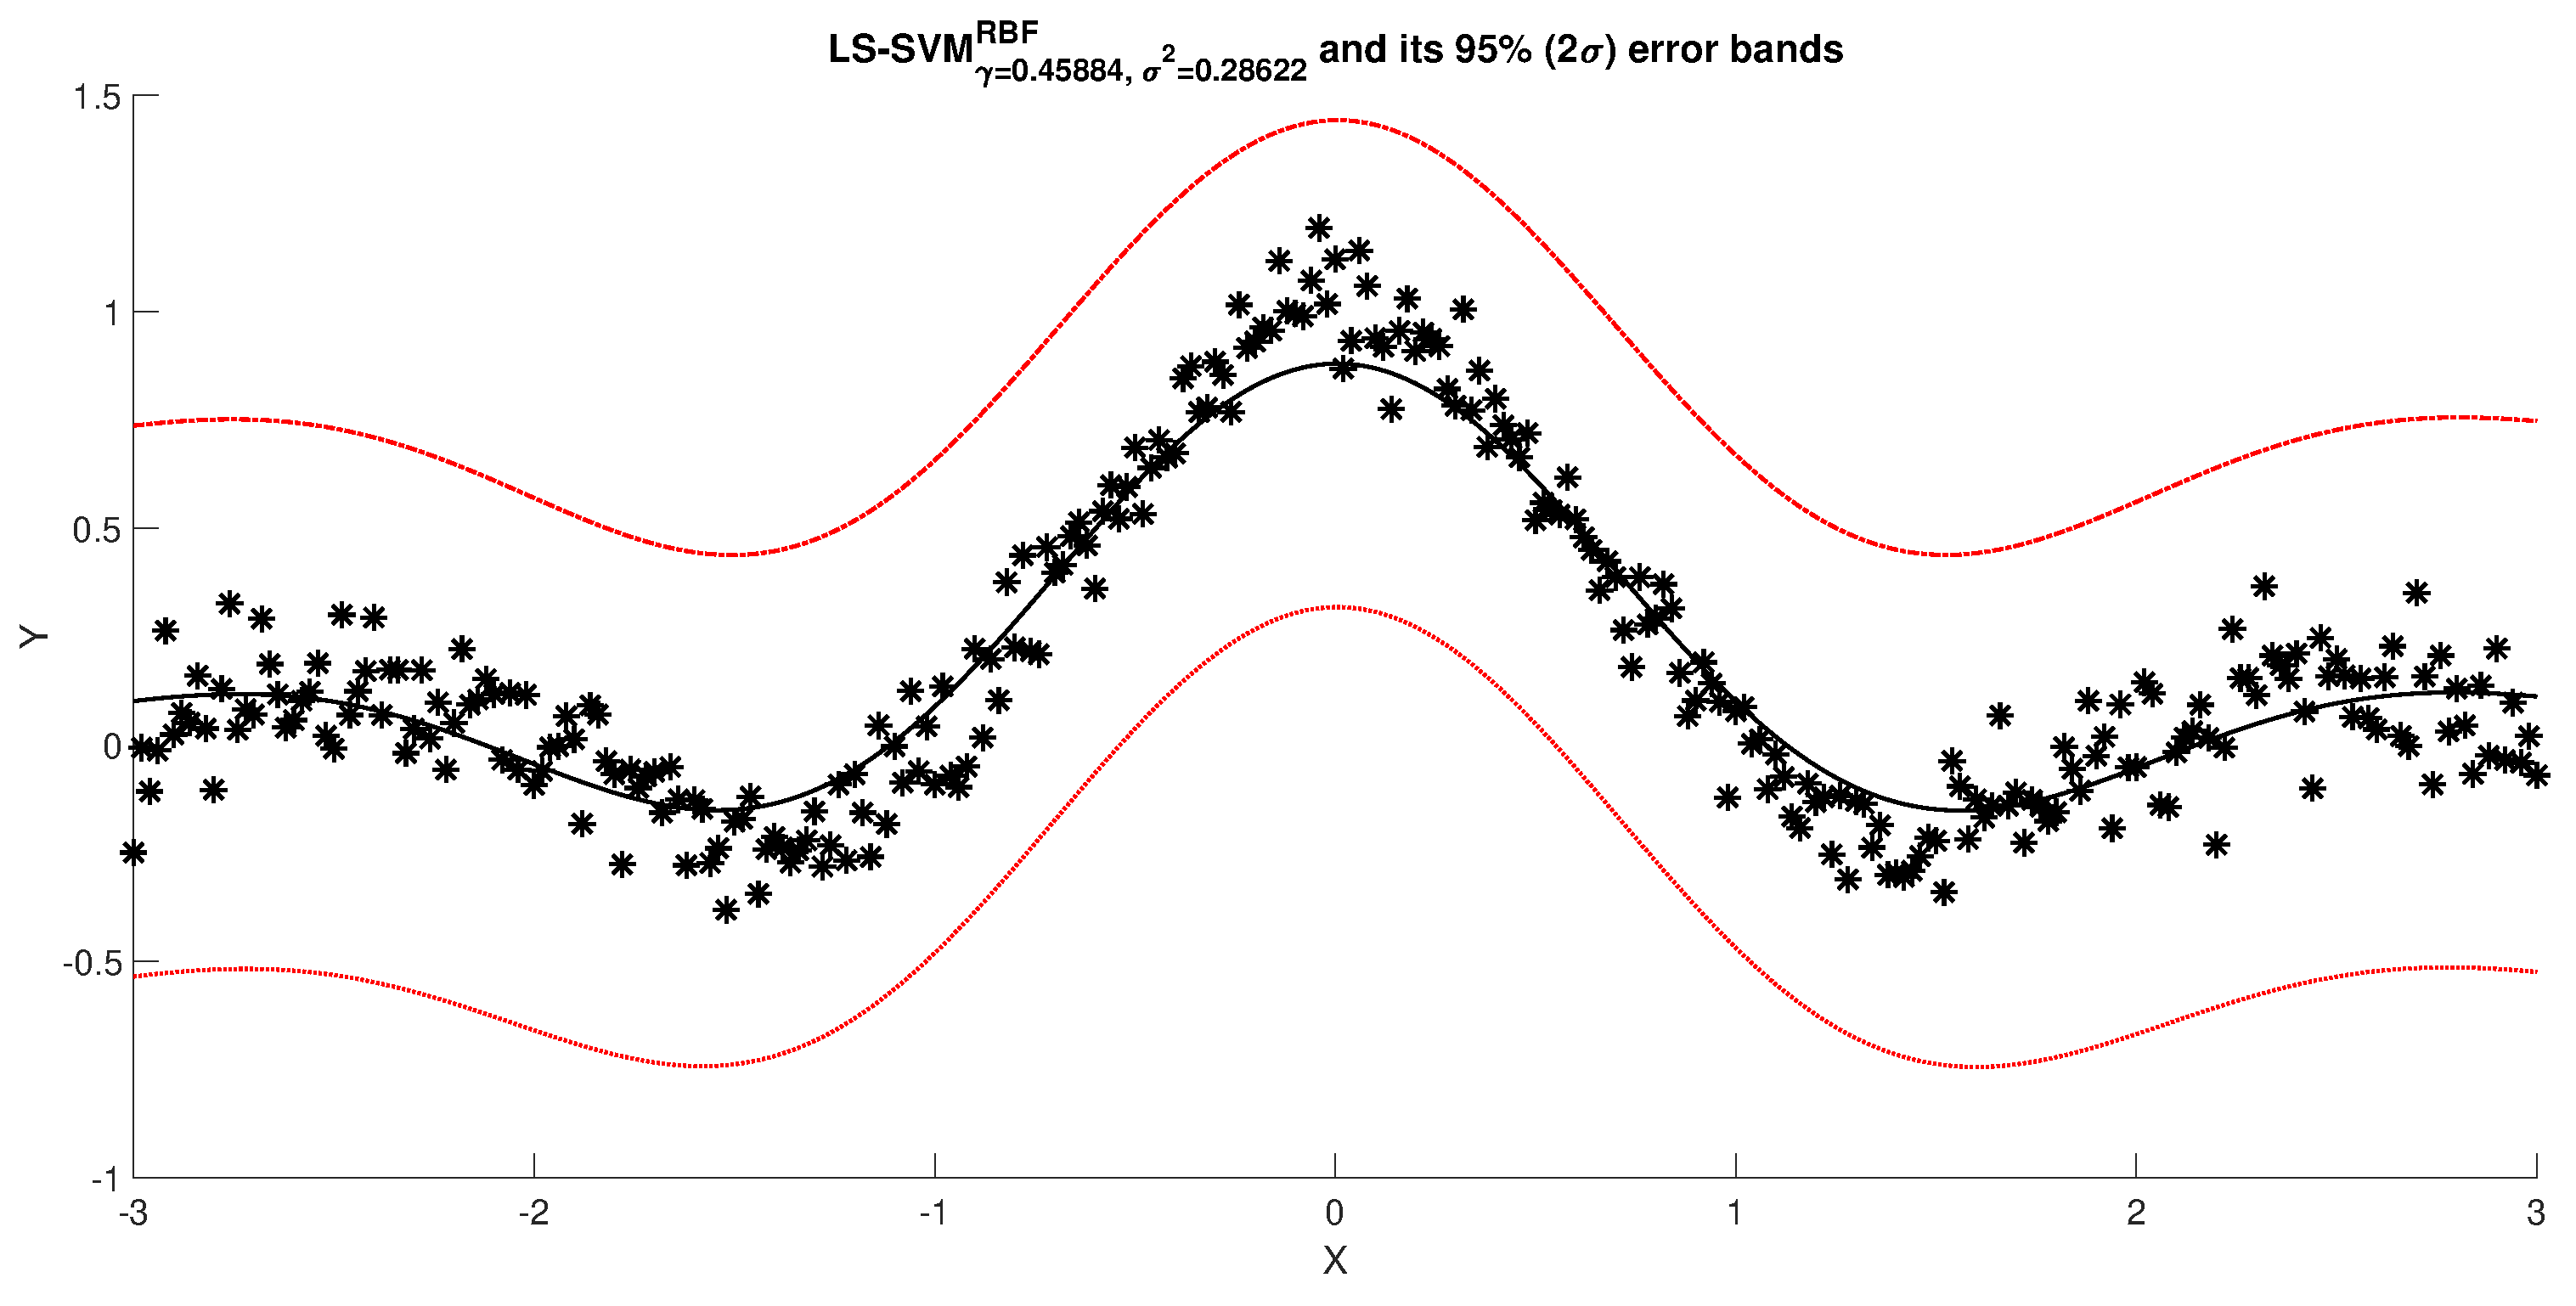
\includegraphics[height = 0.5\linewidth, width=0.8\linewidth]{Exercise2/Report/Bayesian_1.eps}
		\caption{Bayes Framework: LS-SVM with ($\gamma$,$\sigma^2$)=(10,0.4)}
		\label{fig:Bayesian_1}
	\end{subfigure}%
	\begin{subfigure}[b]{0.5\textwidth}
		\centering
		\captionsetup{width=0.7\linewidth}
		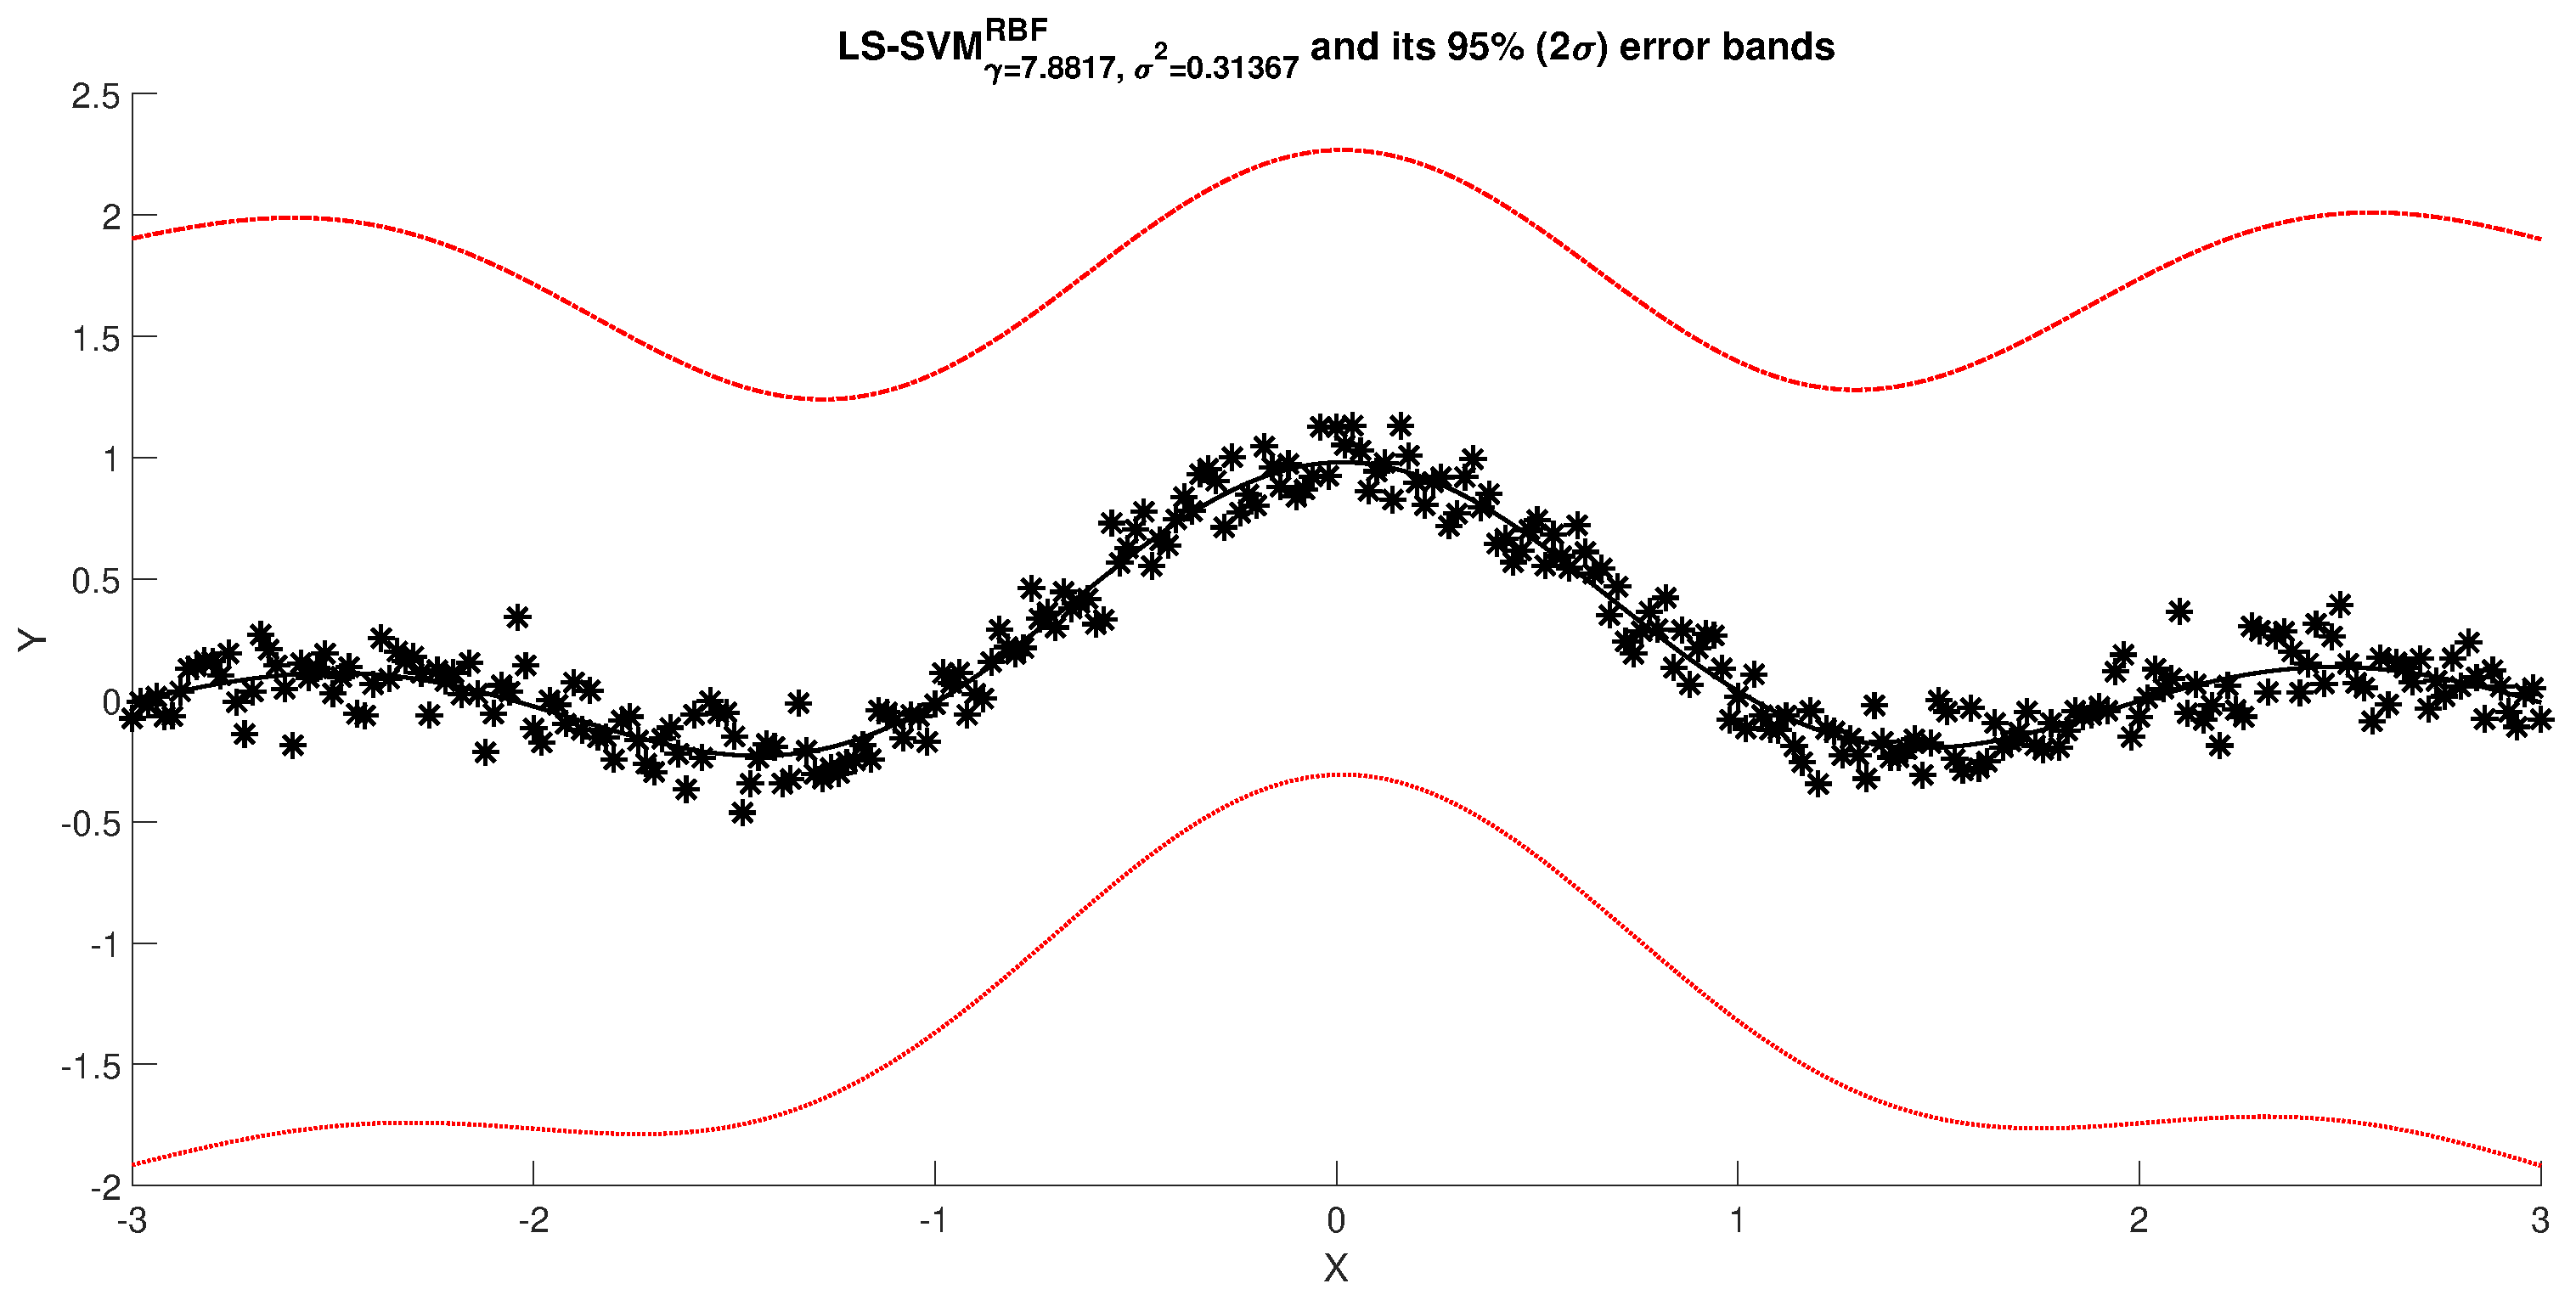
\includegraphics[height = 0.5\linewidth, width=0.8\linewidth]{Exercise2/Report/Bayesian_2.eps}
		\caption{Bayes Framework: LS-SVM with ($\gamma$,$\sigma^2$) obtained from auto tune method}
	\label{fig:Bayesian_2}
	\end{subfigure}

	\caption{Bayesian Framework : LS-SVM }	\label{fig:bayes_1}
\end{figure}
In this section we analyze the function estimation in Bayesian Framework. We first initialize ($\gamma$,$\sigma^2$) values as (10,0.4). We obtain the corresponding posterior parameters as (0.41251, 0.26488) and MSE as 0.1957.  Instead of these random ($\gamma$;$\sigma^2$), we obtain the optimal hyperparameter values using \textit{tunelssvm} with simplex algorithm as (25.6337 ; 0.3815). With these settings we get the posterior parameters as (7.8817; 0.31367) and MSE 0.0423 after bayesian optimization. The corresponding plots are given in figure \ref{fig:bayes_1}.

The optimization in bayesian learning happens in three levels. We assign a probability over all the values of the weight vector $w$ instead of single point of the vector space. For this we need to a prior $p(w)$ and a likelihood                                                                                                                                                                                                                                                                                                                                                                                                                                                                                                                                                                                                                                                                                                                                                                                                                                                                                                                                                                                                                                                                                                                                                                                                                                                                                                                                                                                                                                                                                                                                                                                                                                                                                                                                                                                                                                                                                                                                                                                                                                                                                                                                                                                                                                                                                                                                                                                                                                                                                                                                                                                                                                                                                                                                                                                                                                        probabilities $p(D|w)$ over the data distribution $D$. The posterior probability distribution  can be obtained from prior and likelihood as $P(w|D)=\frac{P(D|w)P(w)}{P(D}$.

\textbf{Level 1:} The main objective here is to minimize the weight space parameters $w$ and $b$. The LS-SVM also includes the regularization hyperparameters $\mu$ and $\zeta$ in its objective function as shown in the below equation \ref{eq:2.1}. Here the optimization is done for $w$ and the bias $b$.

\begin{equation}\label{eq:2.1}
\min\limits_{w,b,e_c} J_P(w,e_c) = \mu \frac{1}{2}w^Tw + \zeta \sum_{k=1}^{N}e_{c,k}^2
\end{equation} 
In the above equation the first term corresponds to prior distribution and the second term corresponds to the likelihood. The posterior distribution and the model $H_\sigma$ is given by:

\begin{equation}\label{eq:2.2}
p(w,b|D,\mu,\zeta,H_\sigma) = \frac{p(D|w,b,\mu,\zeta,H_\sigma)}{p(D|\mu,\zeta,H_\sigma)}p(w,b|\mu,\zeta,H_\sigma)
\end{equation}
Minimization of equation \ref{eq:2.1} for $\mu$, $w$ and $\zeta$ gives the maximization of equation \ref{eq:2.2}. 

\textbf{Level 2:} The regularization parameters $\mu$ and $\zeta$ are optimized in second level.

\textbf{Level 3:} In level three the optimization is done for the kernel parameters. It can used for model selection. 

Therefore, as shown in figure \ref{fig:Bayesian_2}, it results in a better performance for the bayesian framework when tuned with optimal hyperparameters and optimization as MSE given by that model is very less.
\section{Automatic Relevance Determination}
 \begin{figure}[!ht]
	\begin{floatrow}
		\ffigbox{%
			\centering
				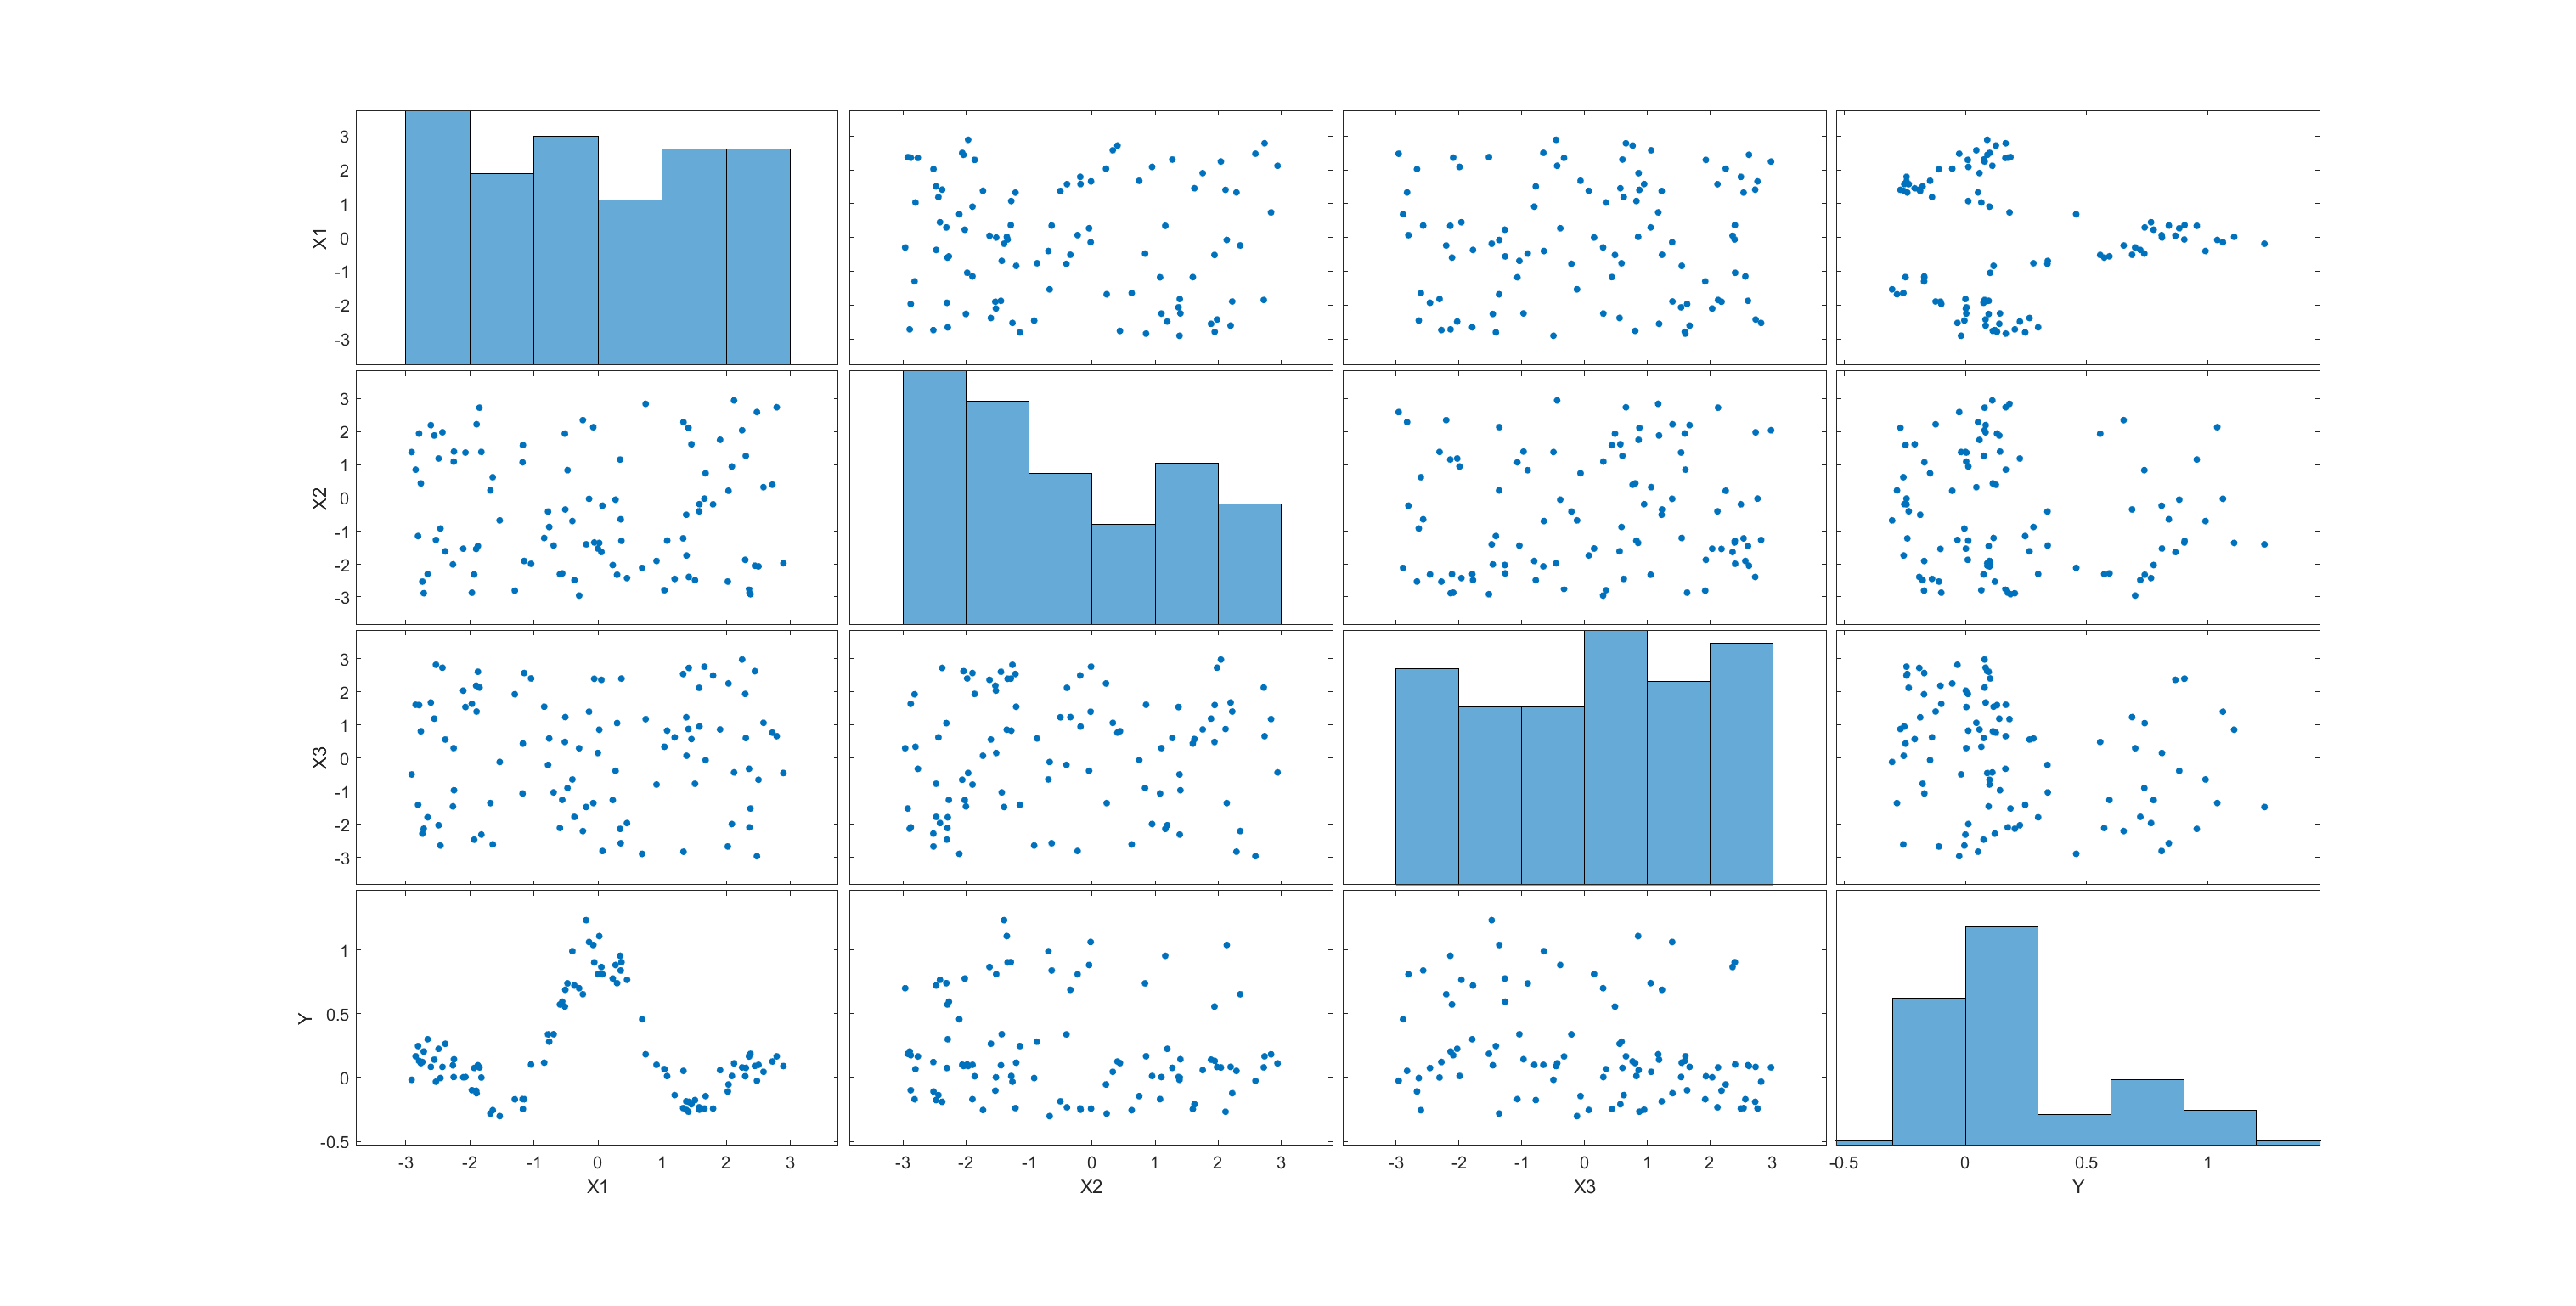
\includegraphics[height = 0.5\textwidth, width = 0.6\textwidth]{Exercise2/Report/Bayes_ARD_1} %
		}{%
			
			\caption{Data distribution}\label{fig:Bayes_ARD_1}%
		}
		\ffigbox{%
			\begin{subfigure}[b]{0.35\textwidth}
				\centering
				\captionsetup{width=1\linewidth}
				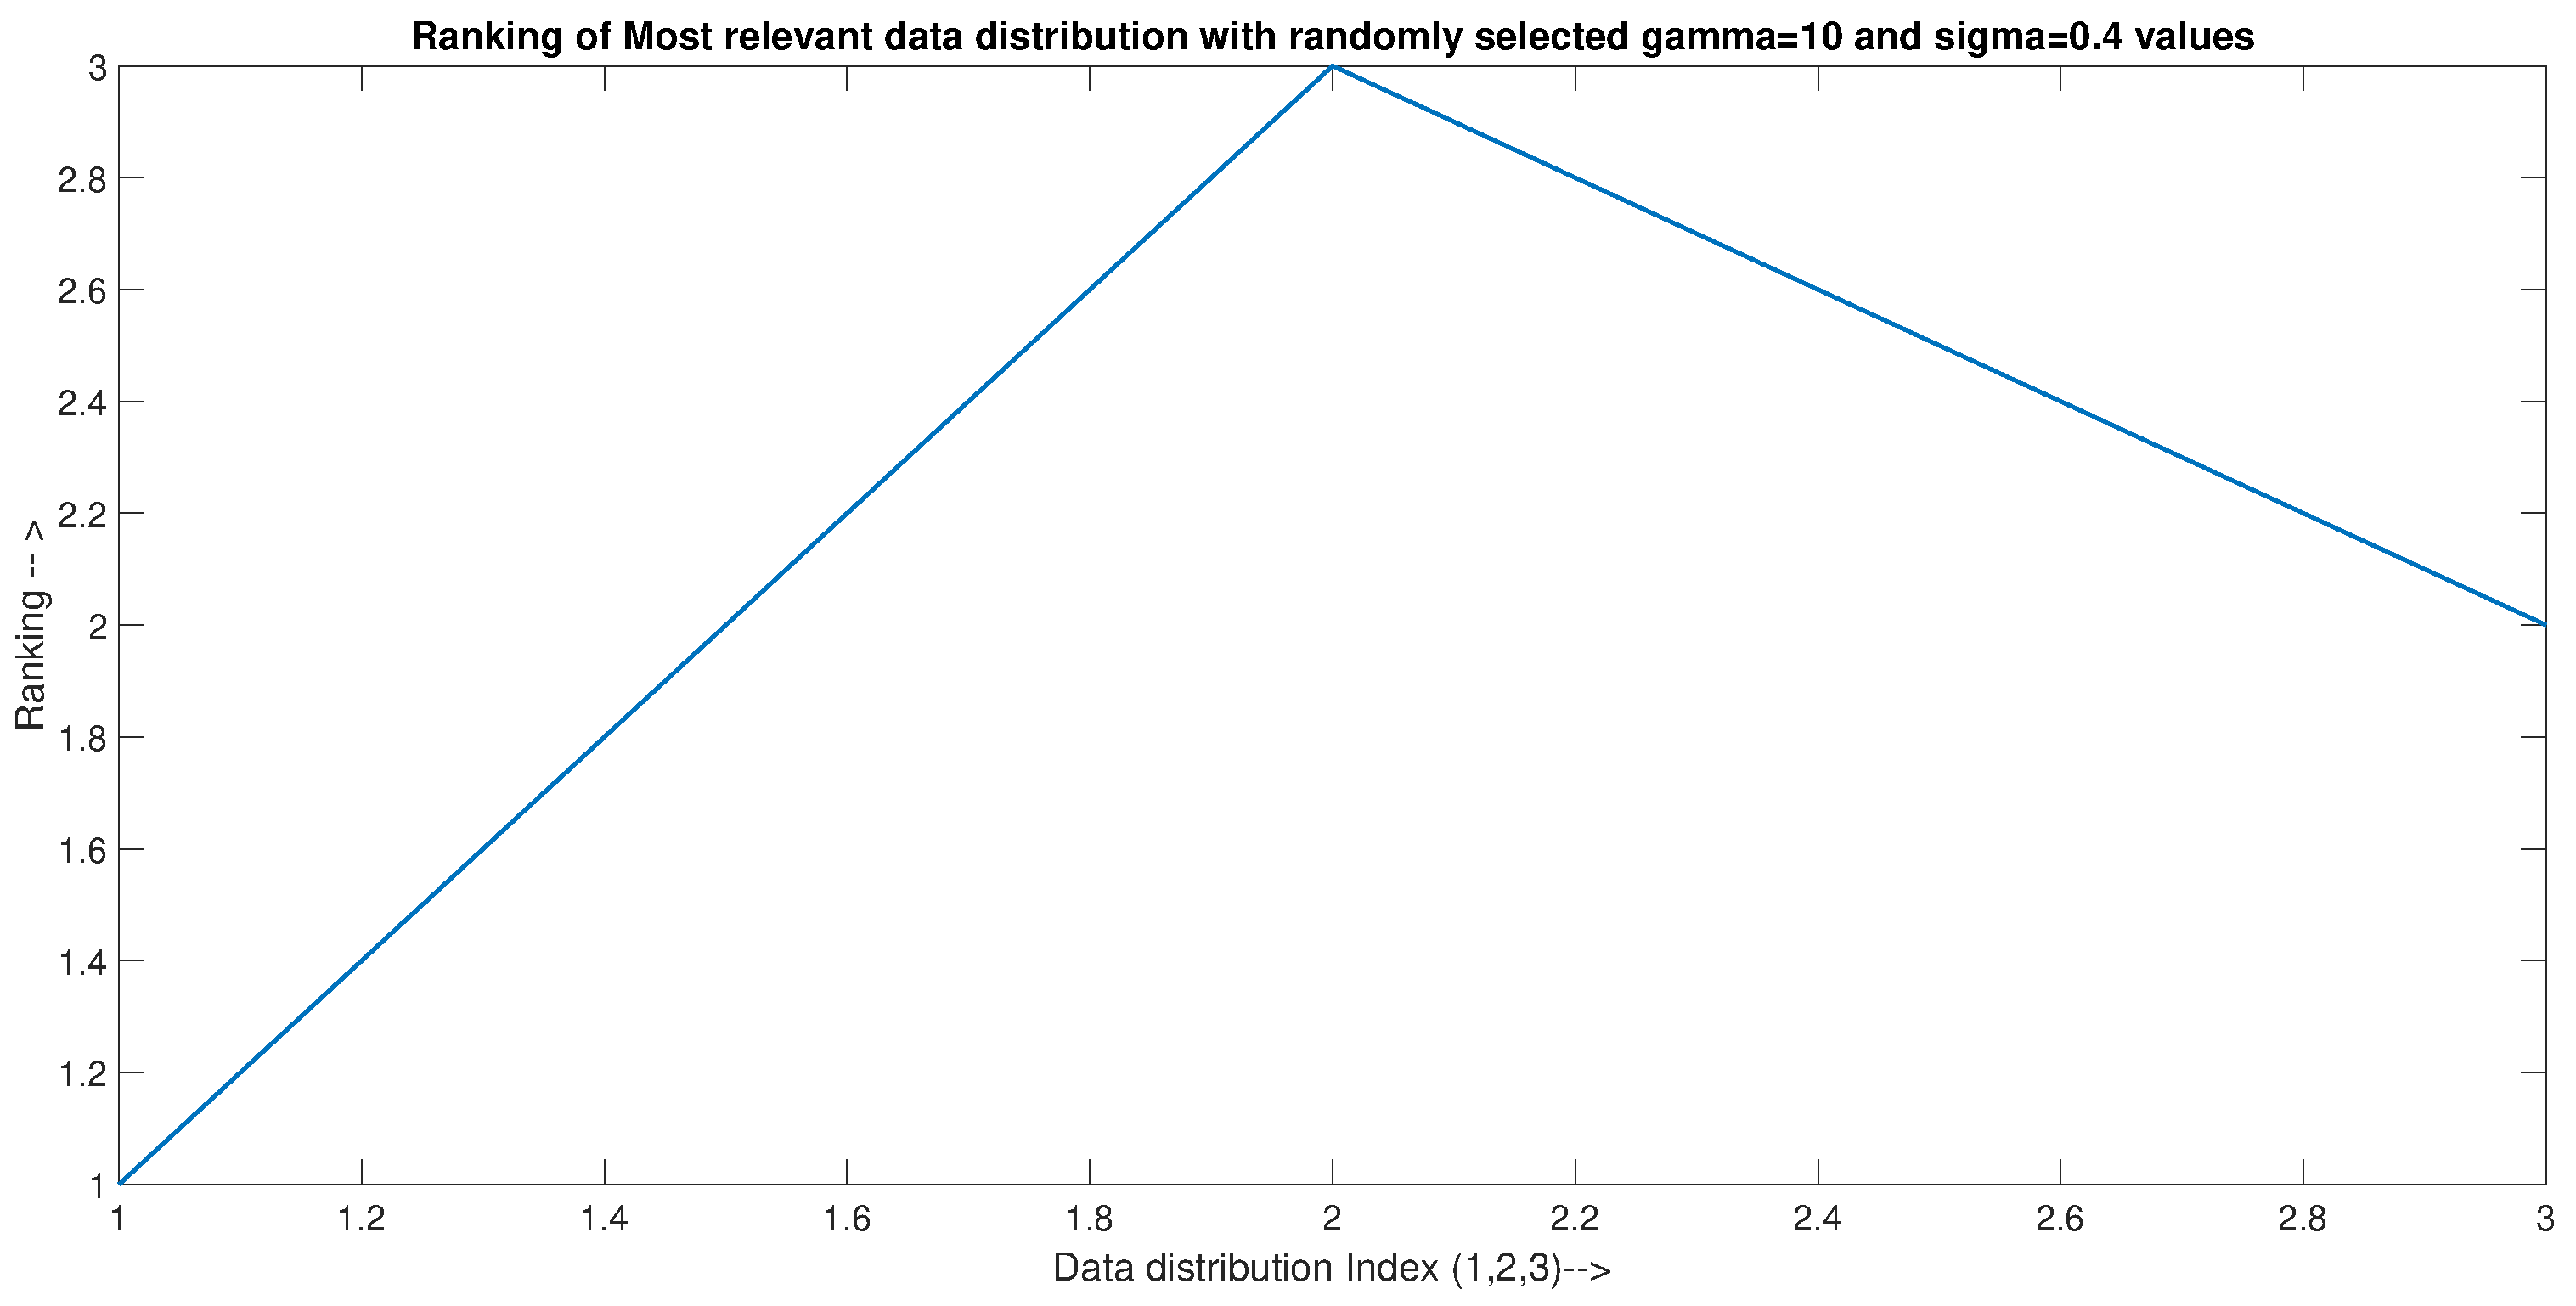
\includegraphics[width = 1\textwidth]{Exercise2/Report/Bayes_ARD_2}
				\caption{Bayes ARD ranking for ($\gamma$;$\sigma^2$)=(10,0.4)}\label{fig:Bayes_ARD_2}
			\end{subfigure}
			\begin{subfigure}[b]{0.35\textwidth}
				\centering
				\captionsetup{width=1\linewidth}
				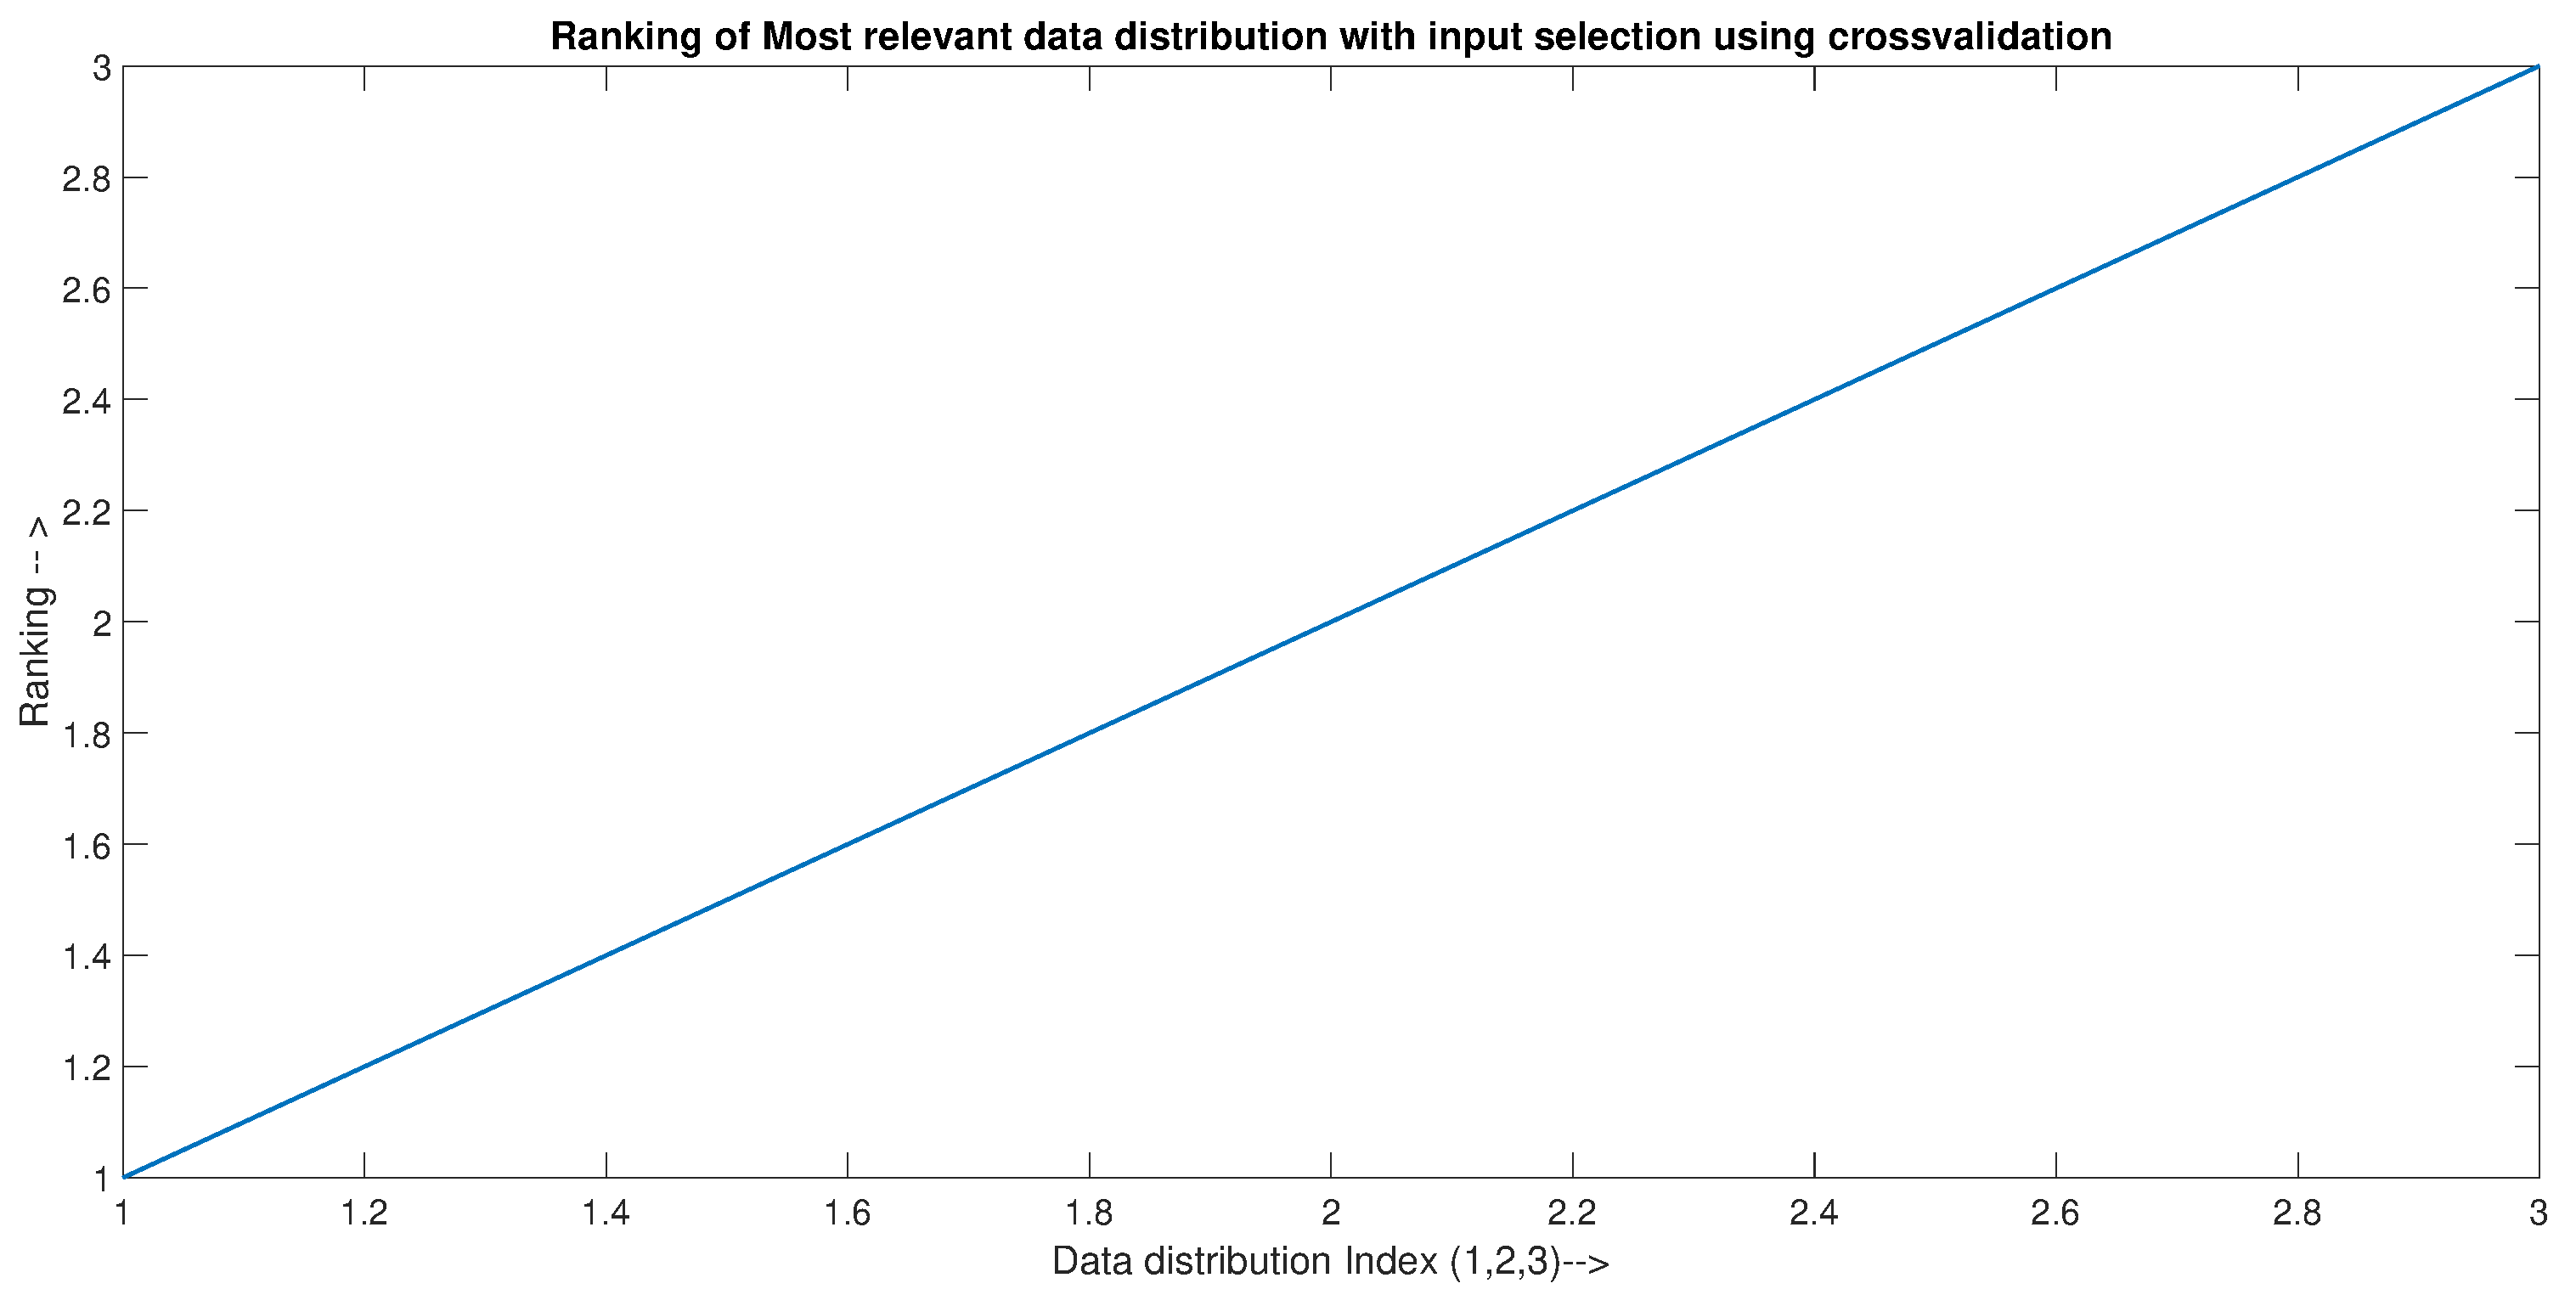
\includegraphics[width = 1\textwidth]{Exercise2/Report/Bayes_ARD_3}
				\caption{Bayes ARD ranking for ($\gamma$;$\sigma^2$) selected from cross validation}\label{fig:Bayes_ARD_3}
			\end{subfigure}			
		}{%
		\caption{Bayes : ARD}
		\label{fig:Bayes_ARD}
		}
	\end{floatrow}
\end{figure}
The Automatic Relevance Distribution ranks the best input data distribution that fits the target by estimating the hyper parameters. To illustrate this, we build three random data distributions X1, X2 and X3.The target label Y is built from X1. The result of figure \ref{fig:Bayes_ARD_2}, is plotted for the model built by randomly choosing ($\gamma$;$\sigma^2$) pair. In figure \ref{fig:Bayes_ARD_3}, the model is built by selecting the inputs using cross validation. As seen from figures \ref{fig:Bayes_ARD_1} and \ref{fig:Bayes_ARD}, the ARD algorithm in both cases gives the data X1 and the most relevant one which is obvious as Y corresponds to X1. Similar results are seen when changing the target Y corresponding to X2 and X3 distributions.   
\section{Robust regression}
\textbf{Visualize and discuss the results. Compare the non-robust version with the robust
	version. Do you spot any differences?}

The figure \ref{fig:robust} shows robust vs non-robust LS-SVM estimations for data points with and without outliers. The non-robust regressor with outliers fail to perform well as the estimations try to take the outliers also into account. This results in a poor fit over the data points as seen in figure \ref{fig:rob_outliers}. On the other hand, the robust regressor with cross validation gives good performance with better function estimations ignoring the outliers as seen in figure \ref{fig:rob_huber}\\\\
\begin{figure}[!ht] 
	\begin{subfigure}{.35\textwidth}
		\centering
		\captionsetup{width=0.8\linewidth}
		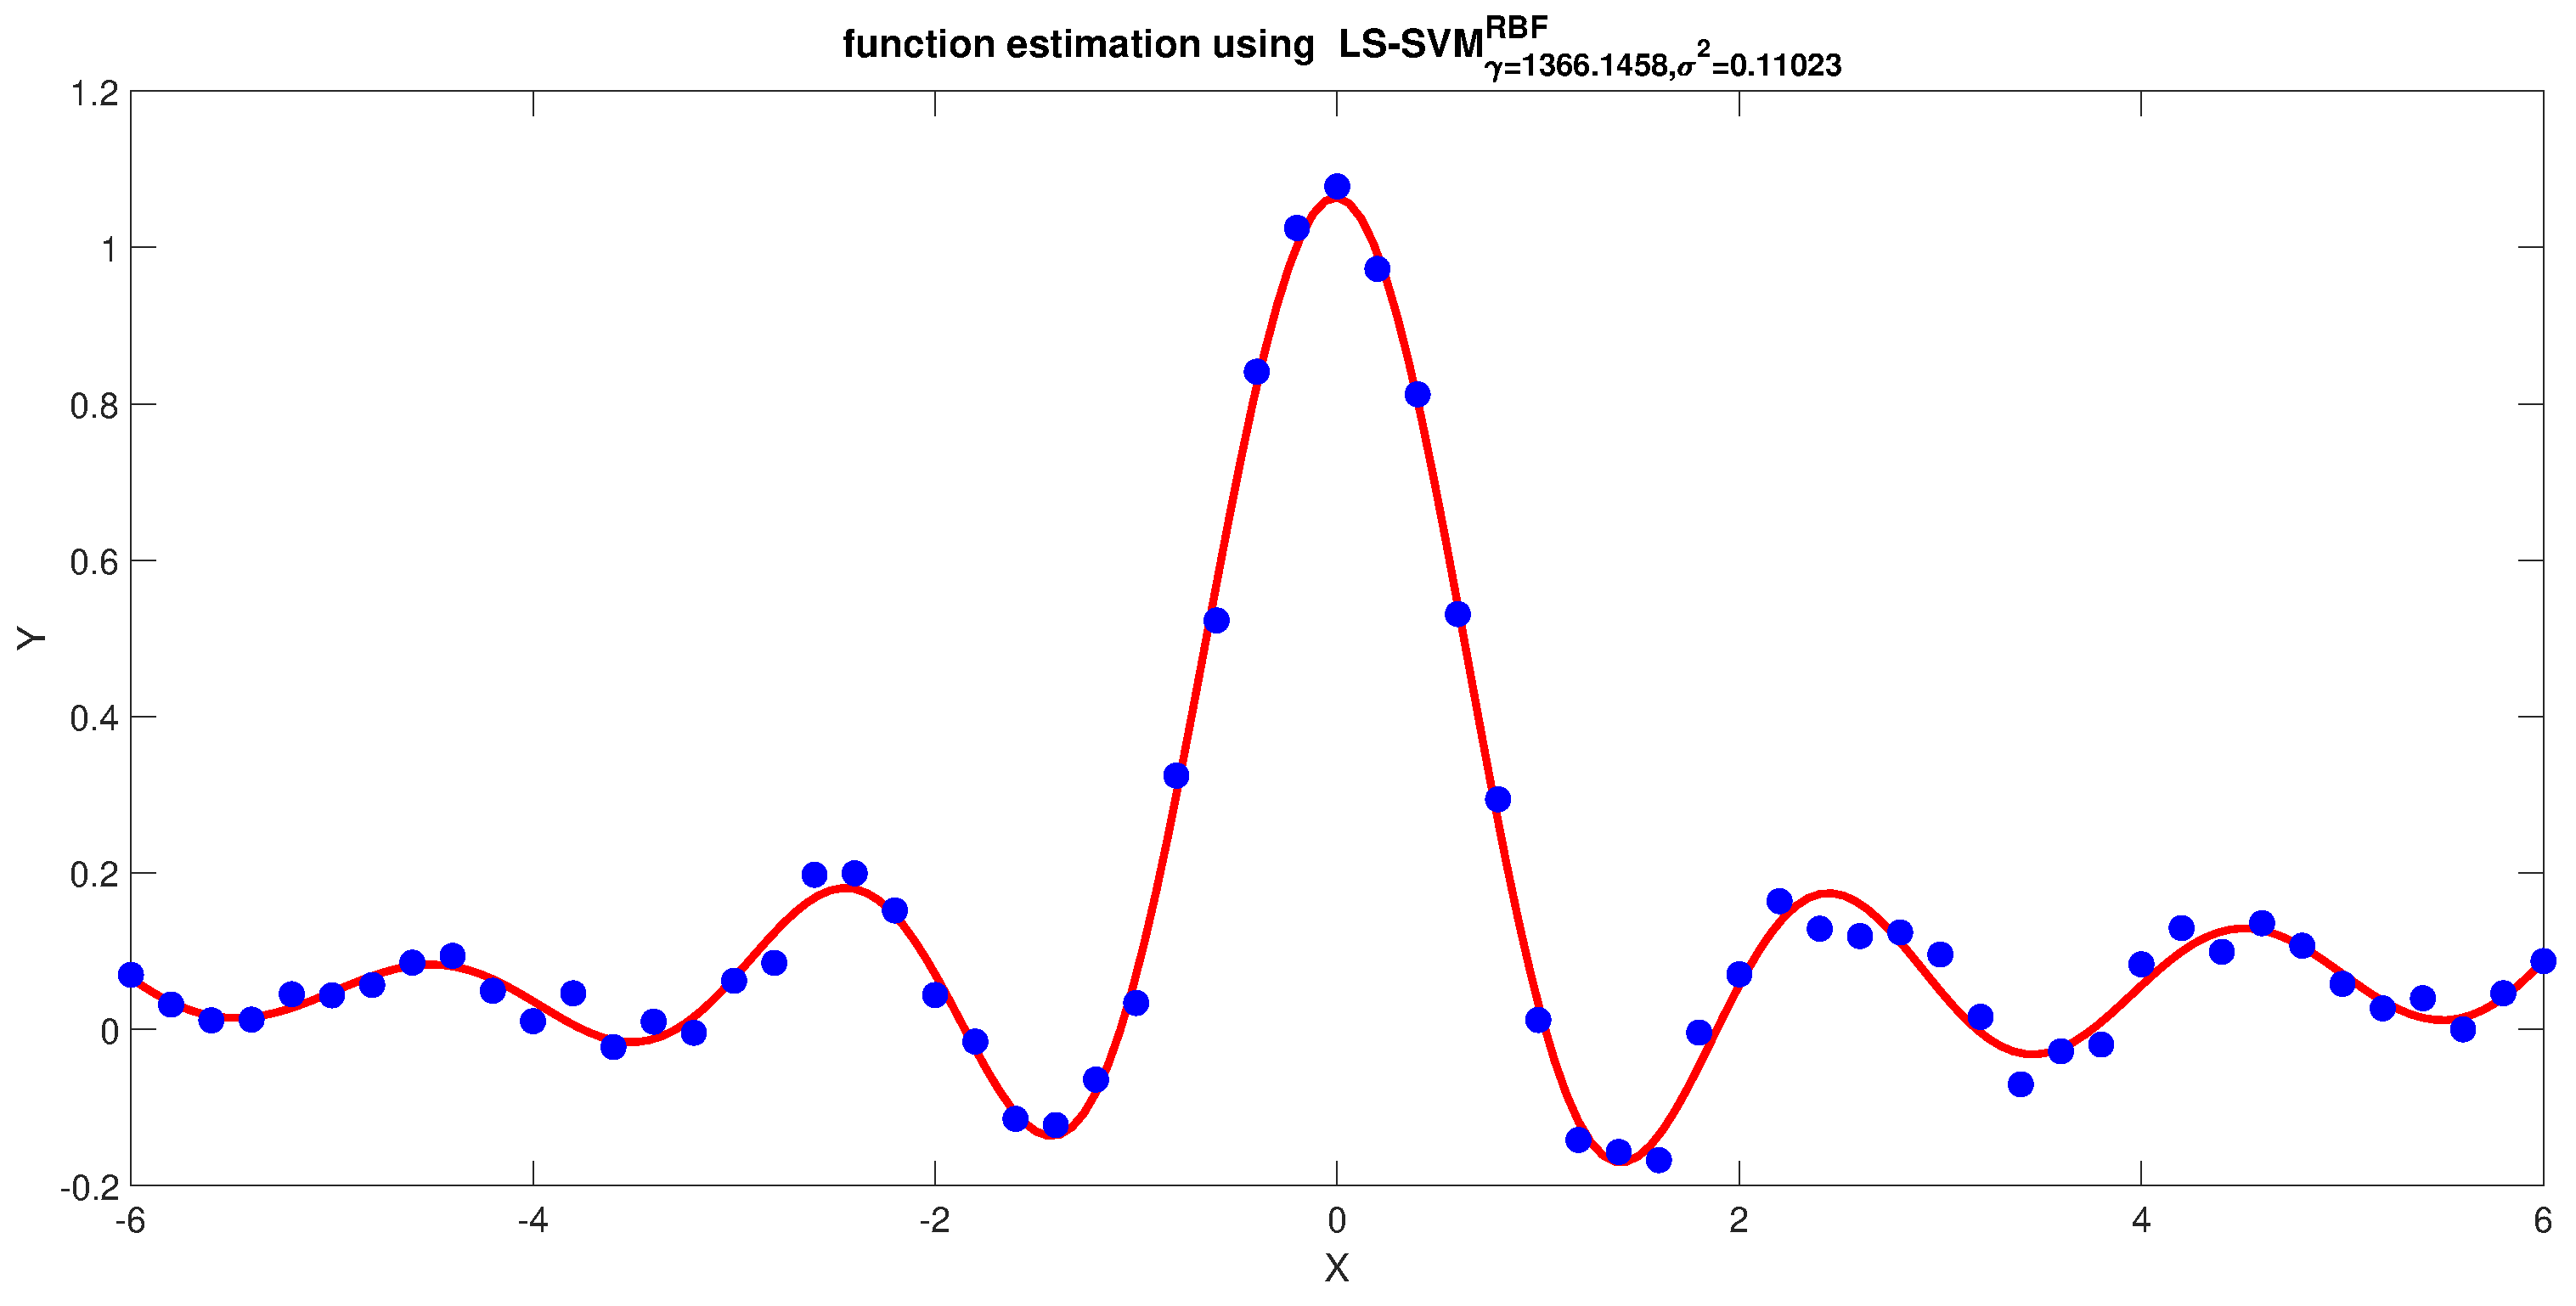
\includegraphics[height=.65\linewidth, width=0.9\linewidth]{Exercise2/Report/robust_withoutOutliers}
		\caption{LS-SVM Regressor : Without Outliers}
		\label{fig:rob_nooutliers}
	\end{subfigure}%
	\begin{subfigure}{.35\textwidth}
		\centering
		\captionsetup{width=0.8\linewidth}
		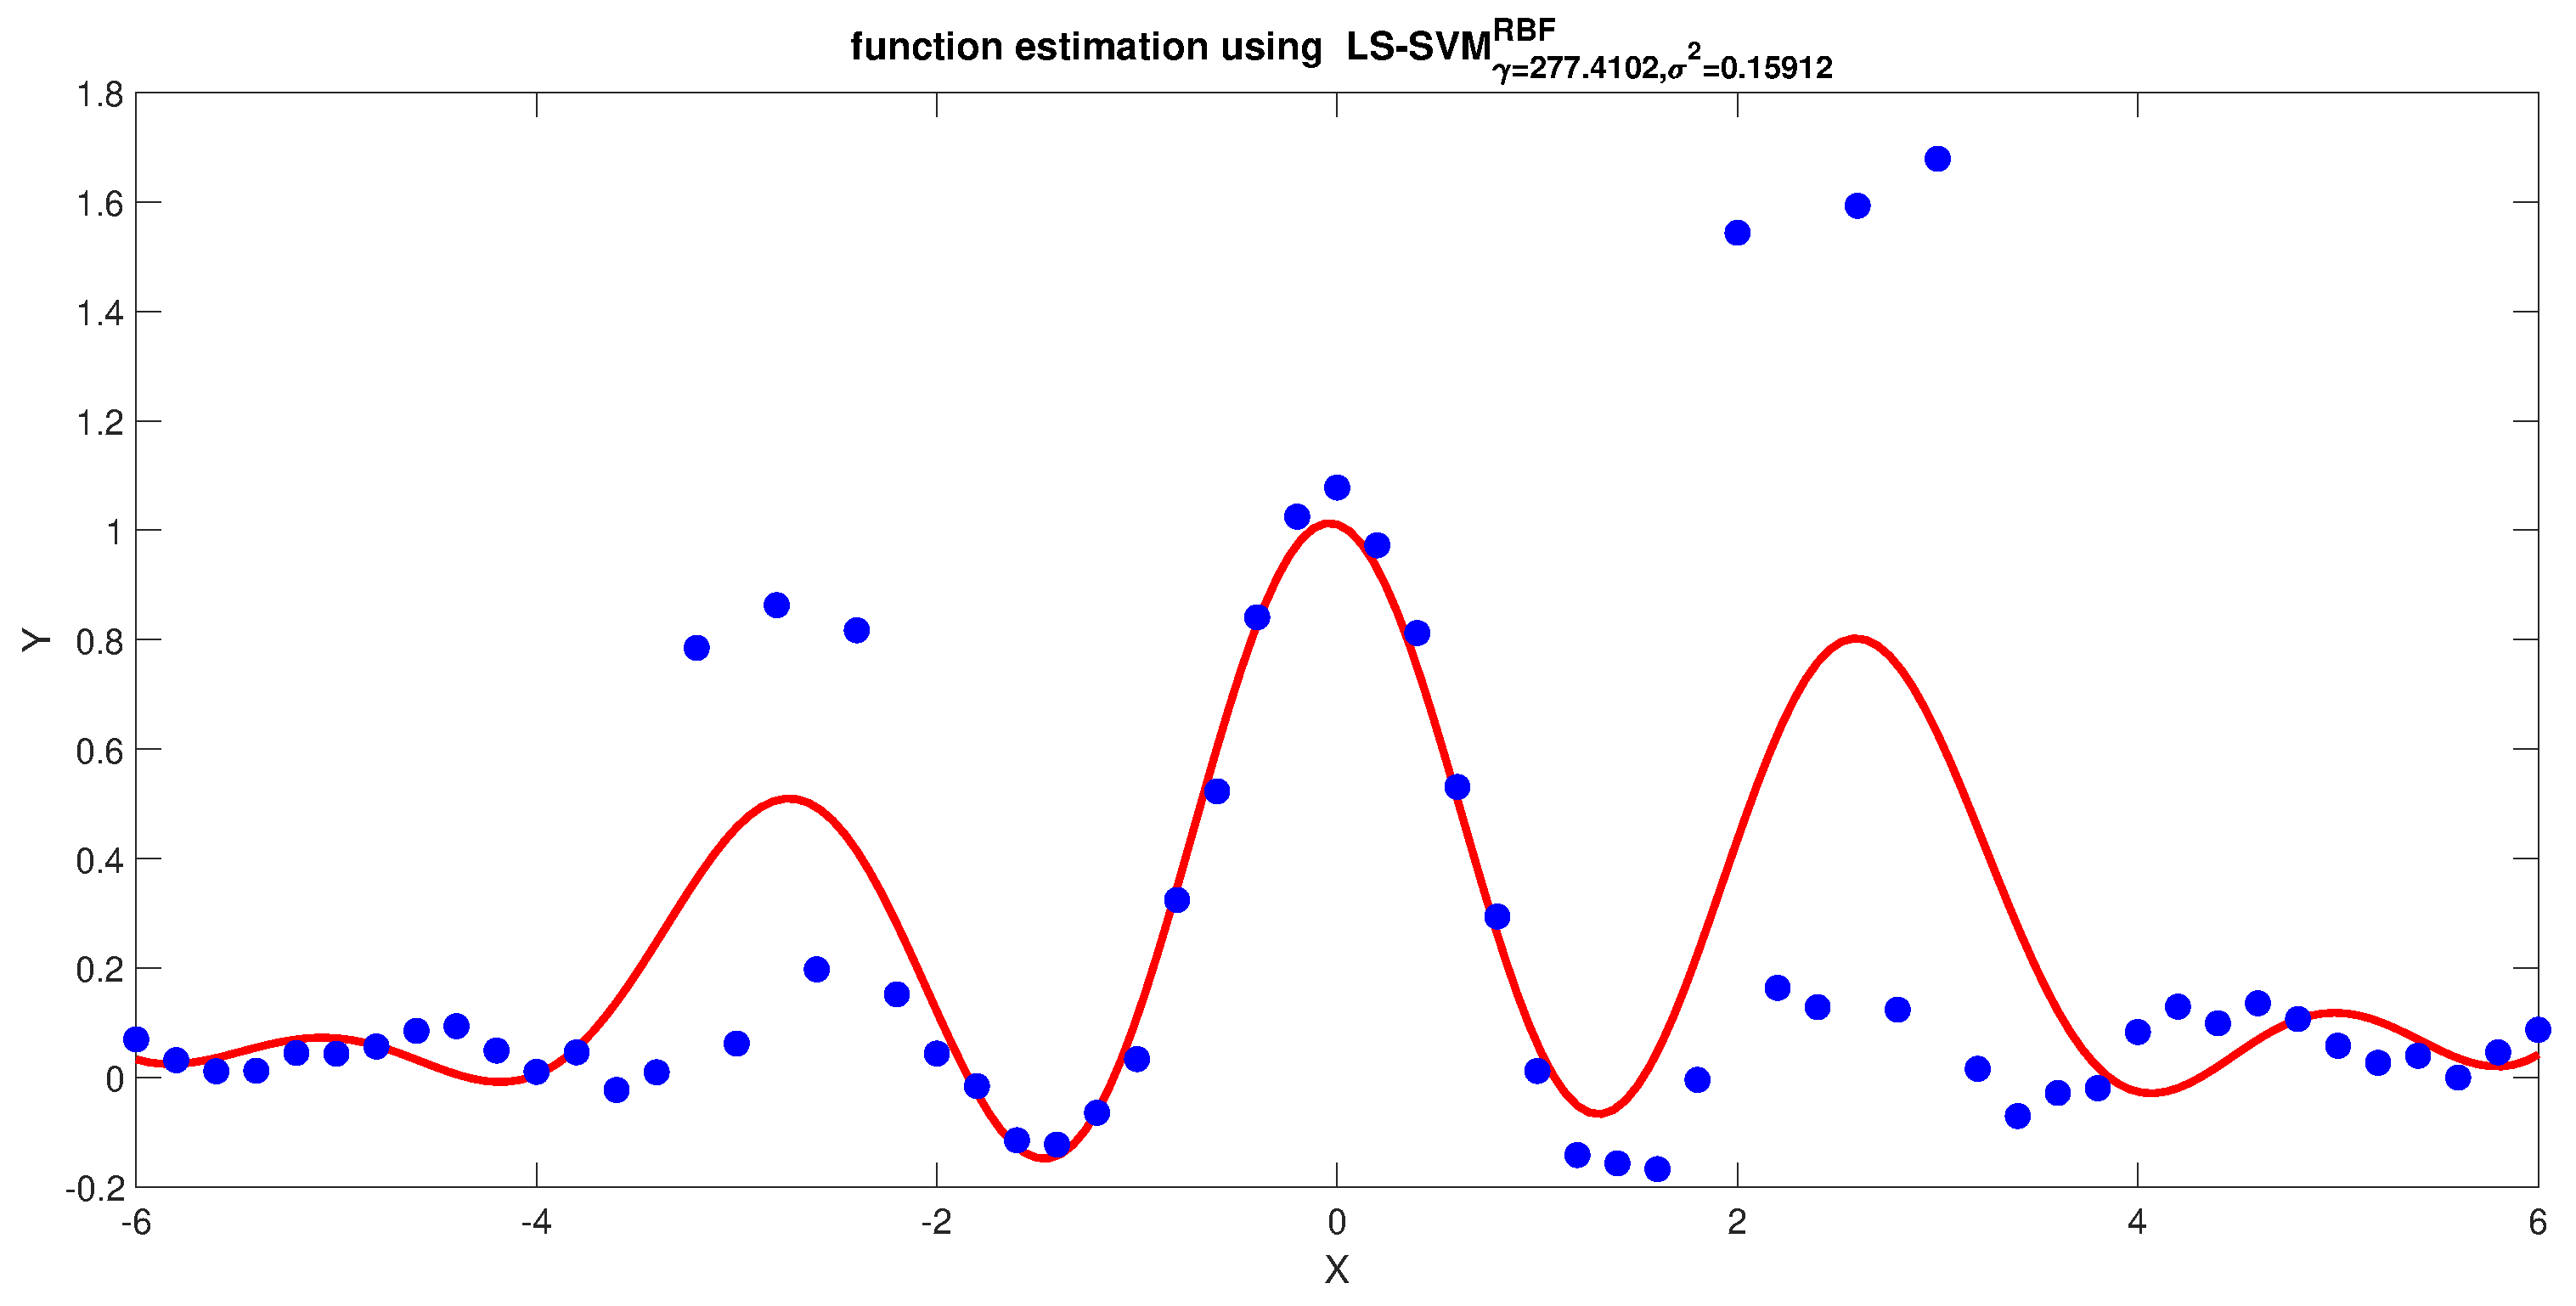
\includegraphics[height=.65\linewidth, width=0.9\linewidth]{Exercise2/Report/robust_withOutliers}
		\caption{LS-SVM Regressor : With Outliers}
		\label{fig:rob_outliers}
	\end{subfigure}%
	\begin{subfigure}{.35\textwidth}
		\centering
		\captionsetup{width=0.8\linewidth}
		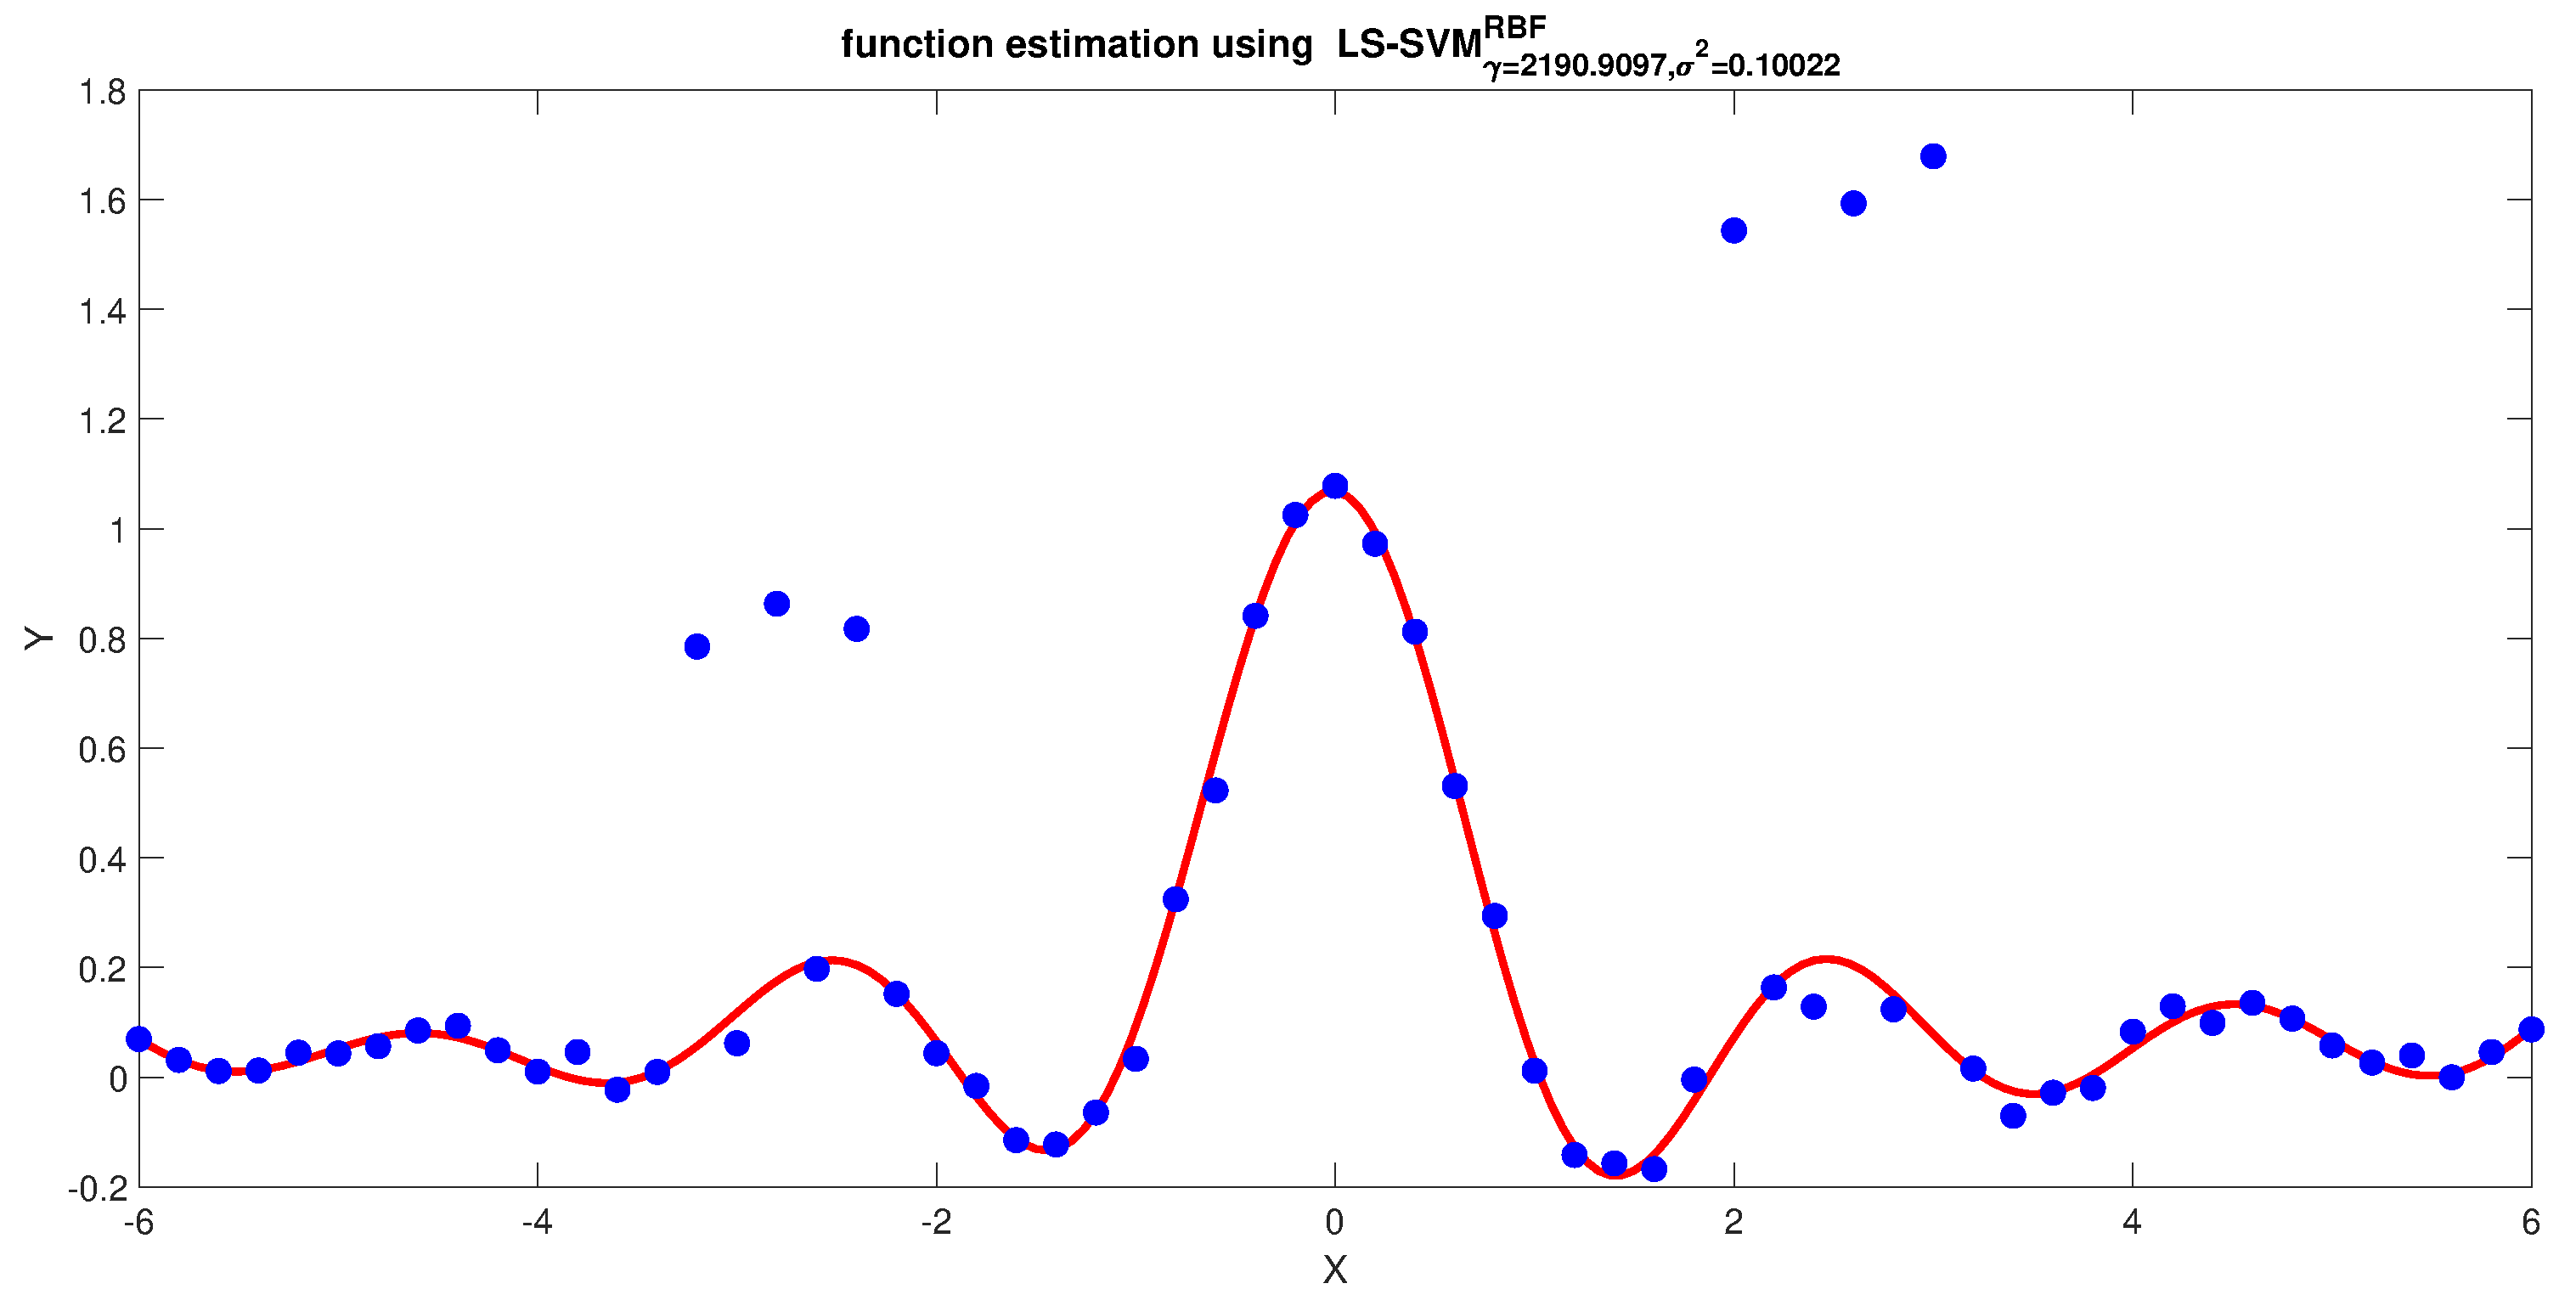
\includegraphics[height=.65\linewidth, width=0.9\linewidth]{Exercise2/Report/robust_huber}
		\caption{LS-SVM Regressor : Robust Cross Validation}
		\label{fig:rob_huber}
	\end{subfigure}
	\caption{LS-SVM : Robust Vs Non-Robust versions}
	\label{fig:robust}
\end{figure}
\textbf{Why in this case is the mean absolute error (’mae’) preferred over the classical mean
	squared error (’mse’)?}

MAE is the measure of average magnitude of errors between true and estimated data points. Whereas MSE is the measure of squared average magnitude of errors. Since, MSE is the squared error, it adds more weight to outliers where the errors are high.This makes the model perform poorly when trying to minimize the errors. This is not the case with MAE as it only takes the absolute average of errors and that makes it more robust to outliers.
\begin{align*}
MAE = \frac{1}{N} \sum_{i=1}^{N} |y_i - \hat{y_i}| && MSE = \frac{1}{N} \sum_{i=1}^{N} (y_i - \hat{y_i})^2 \label{eq:label1}
\end{align*}\\
\textbf{Try alternatives to the weighting function wFun (e.g., ’whampel’, ’wlogistic’ and
	’wmyriad’. Report on differences. Check the user’s guide of LS-SVMlab for more
	information.}
\begin{figure}[!ht] 
	\begin{subfigure}{.35\textwidth}
		\centering
		\captionsetup{width=0.8\linewidth}
		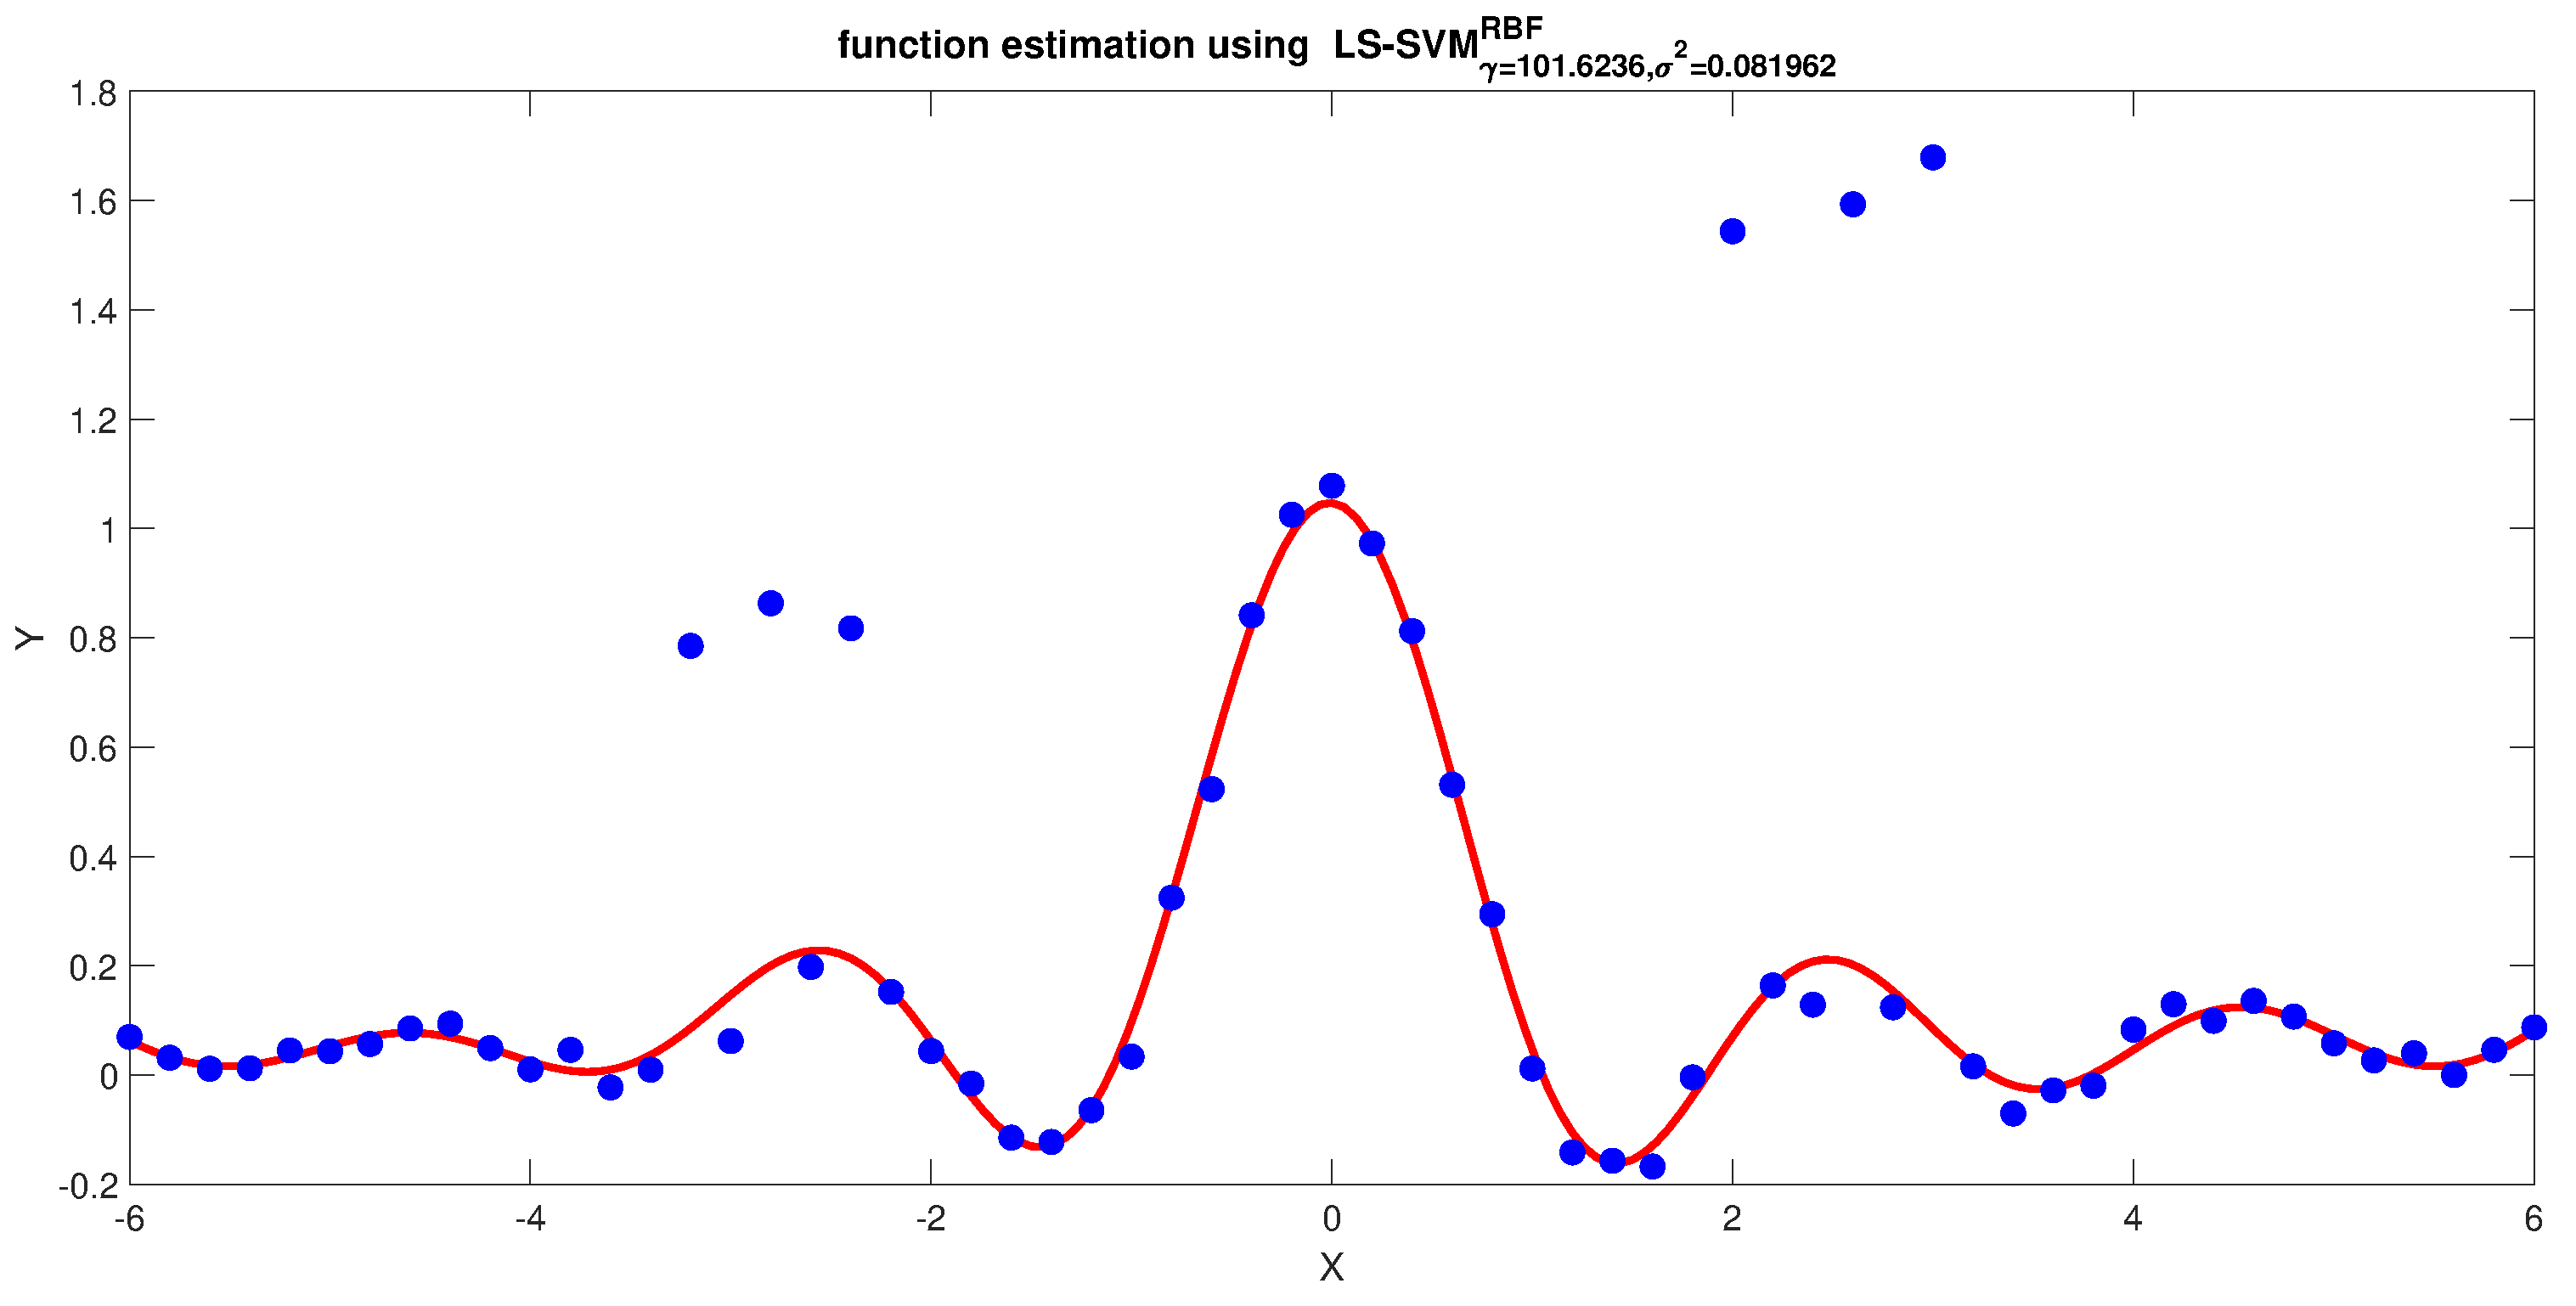
\includegraphics[height=.65\linewidth, width=0.9\linewidth]{Exercise2/Report/robust_logistic}
		\caption{Robust LS-SVM Regressor : Logistic}
		\label{fig:rob_nooutliers}
	\end{subfigure}%
	\begin{subfigure}{.35\textwidth}
		\centering
		\captionsetup{width=0.8\linewidth}
		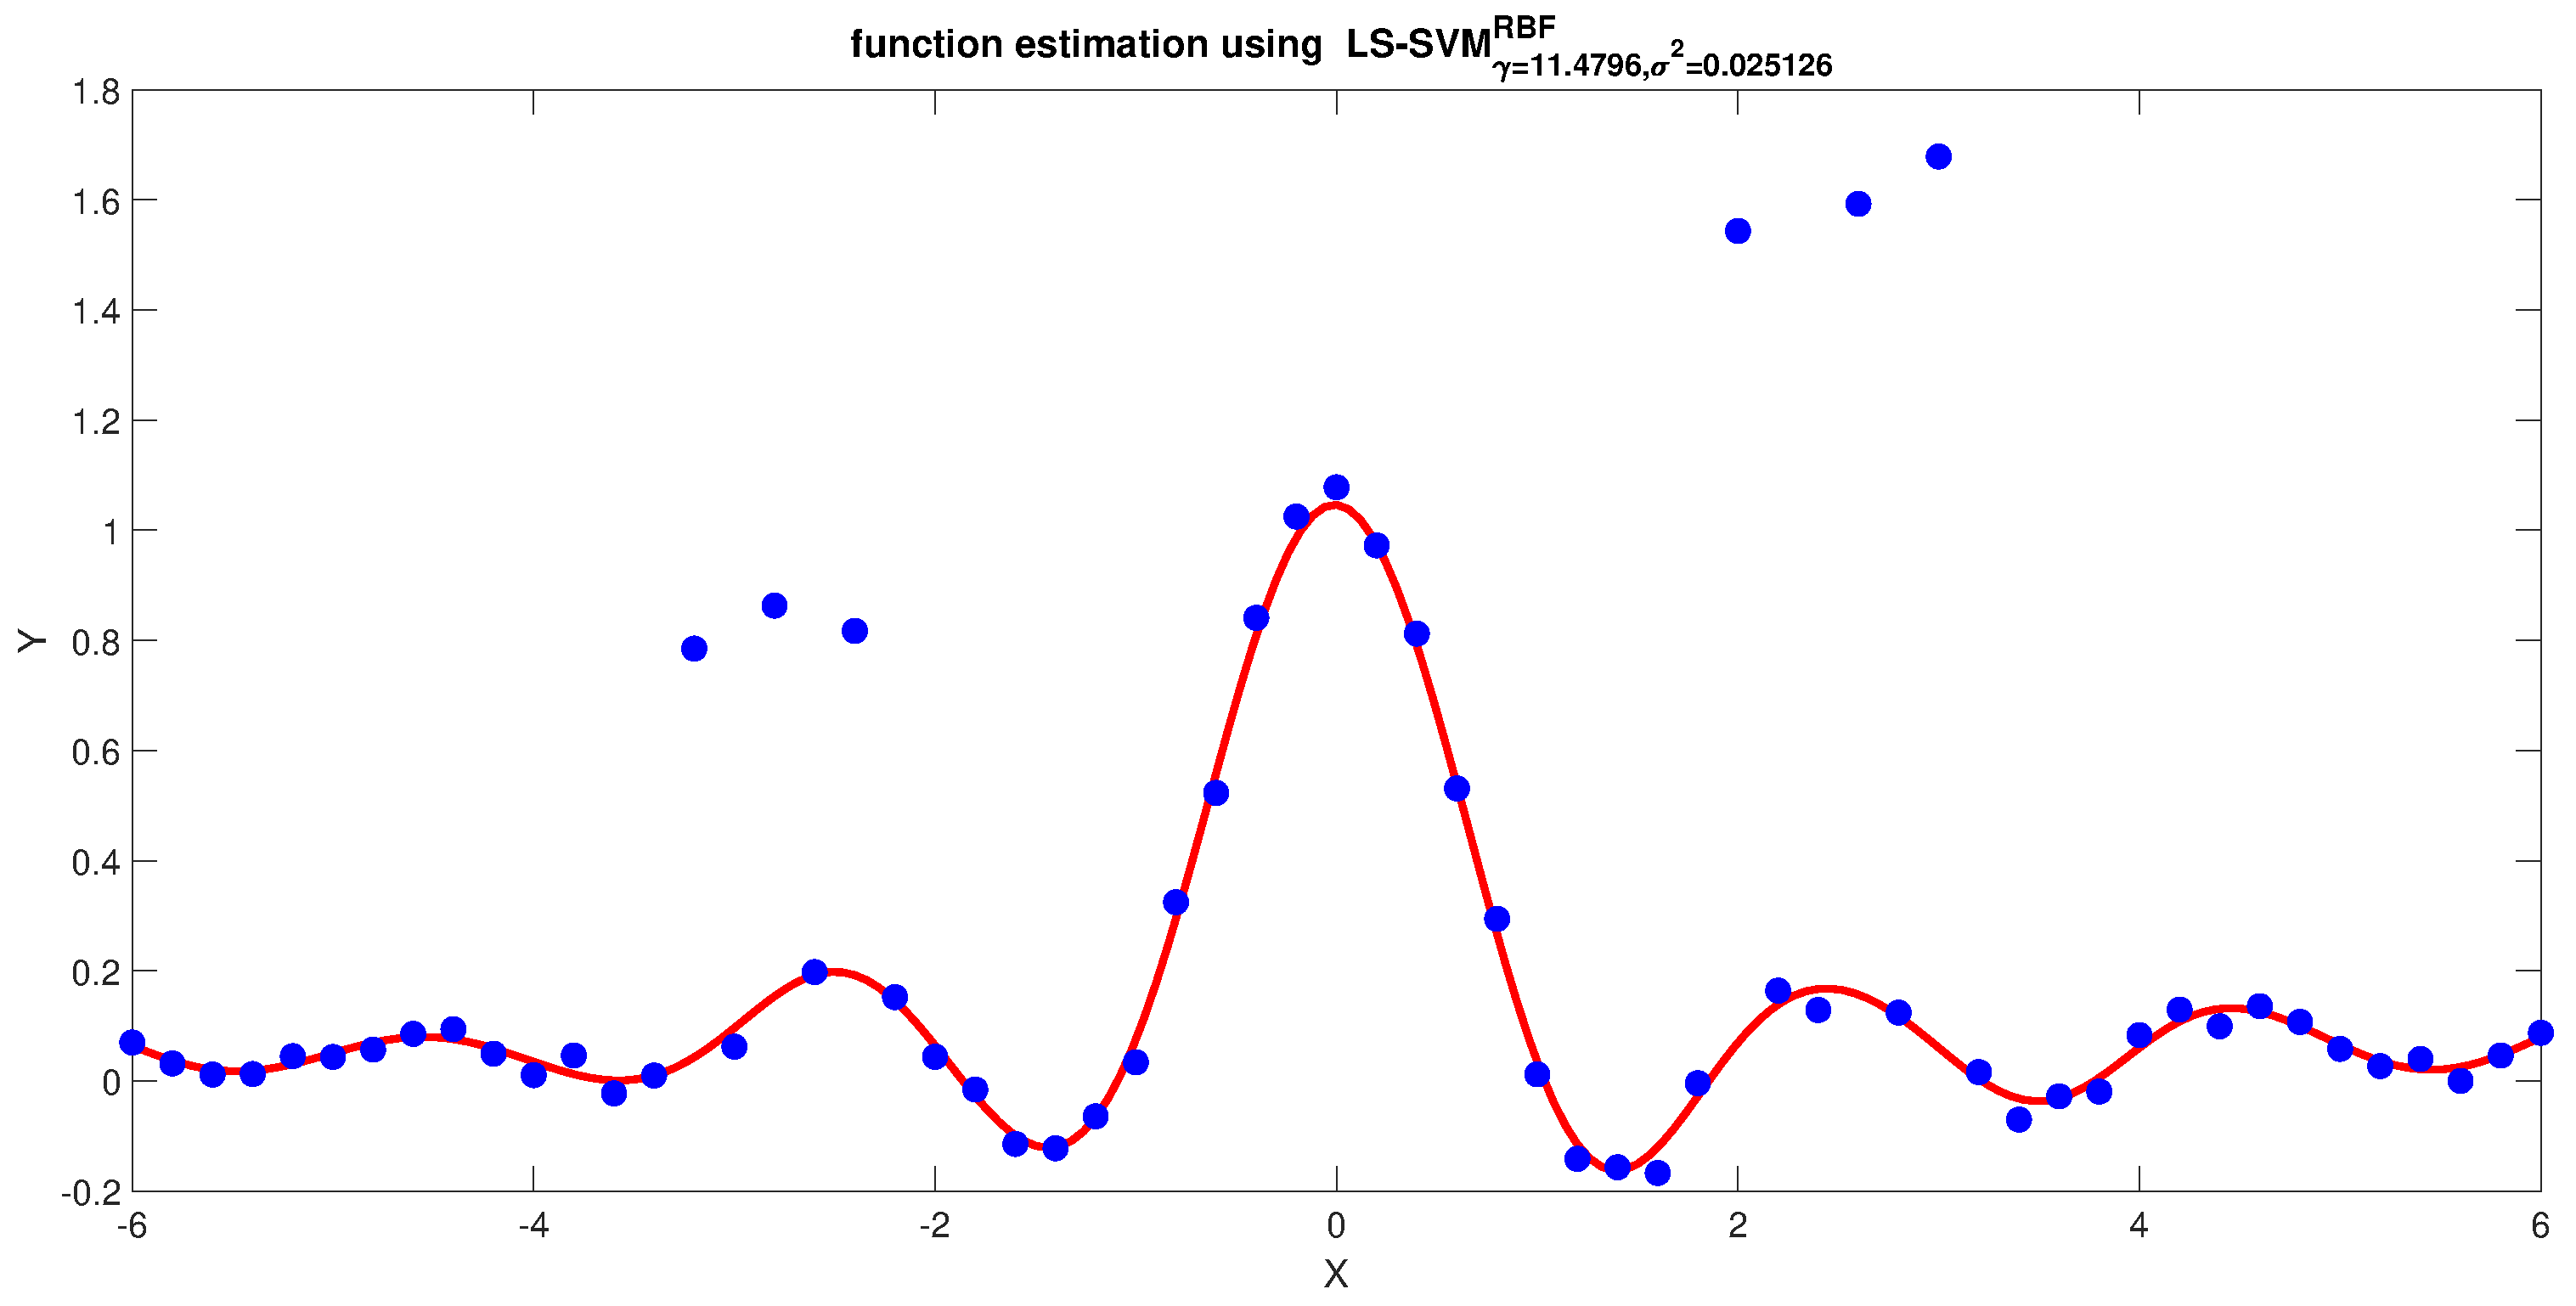
\includegraphics[height=.65\linewidth, width=0.9\linewidth]{Exercise2/Report/robust_myriad}
		\caption{Robust LS-SVM Regressor : Myriad}
		\label{fig:rob_myriad}
	\end{subfigure}%
	\begin{subfigure}{.35\textwidth}
		\centering
		\captionsetup{width=0.8\linewidth}
		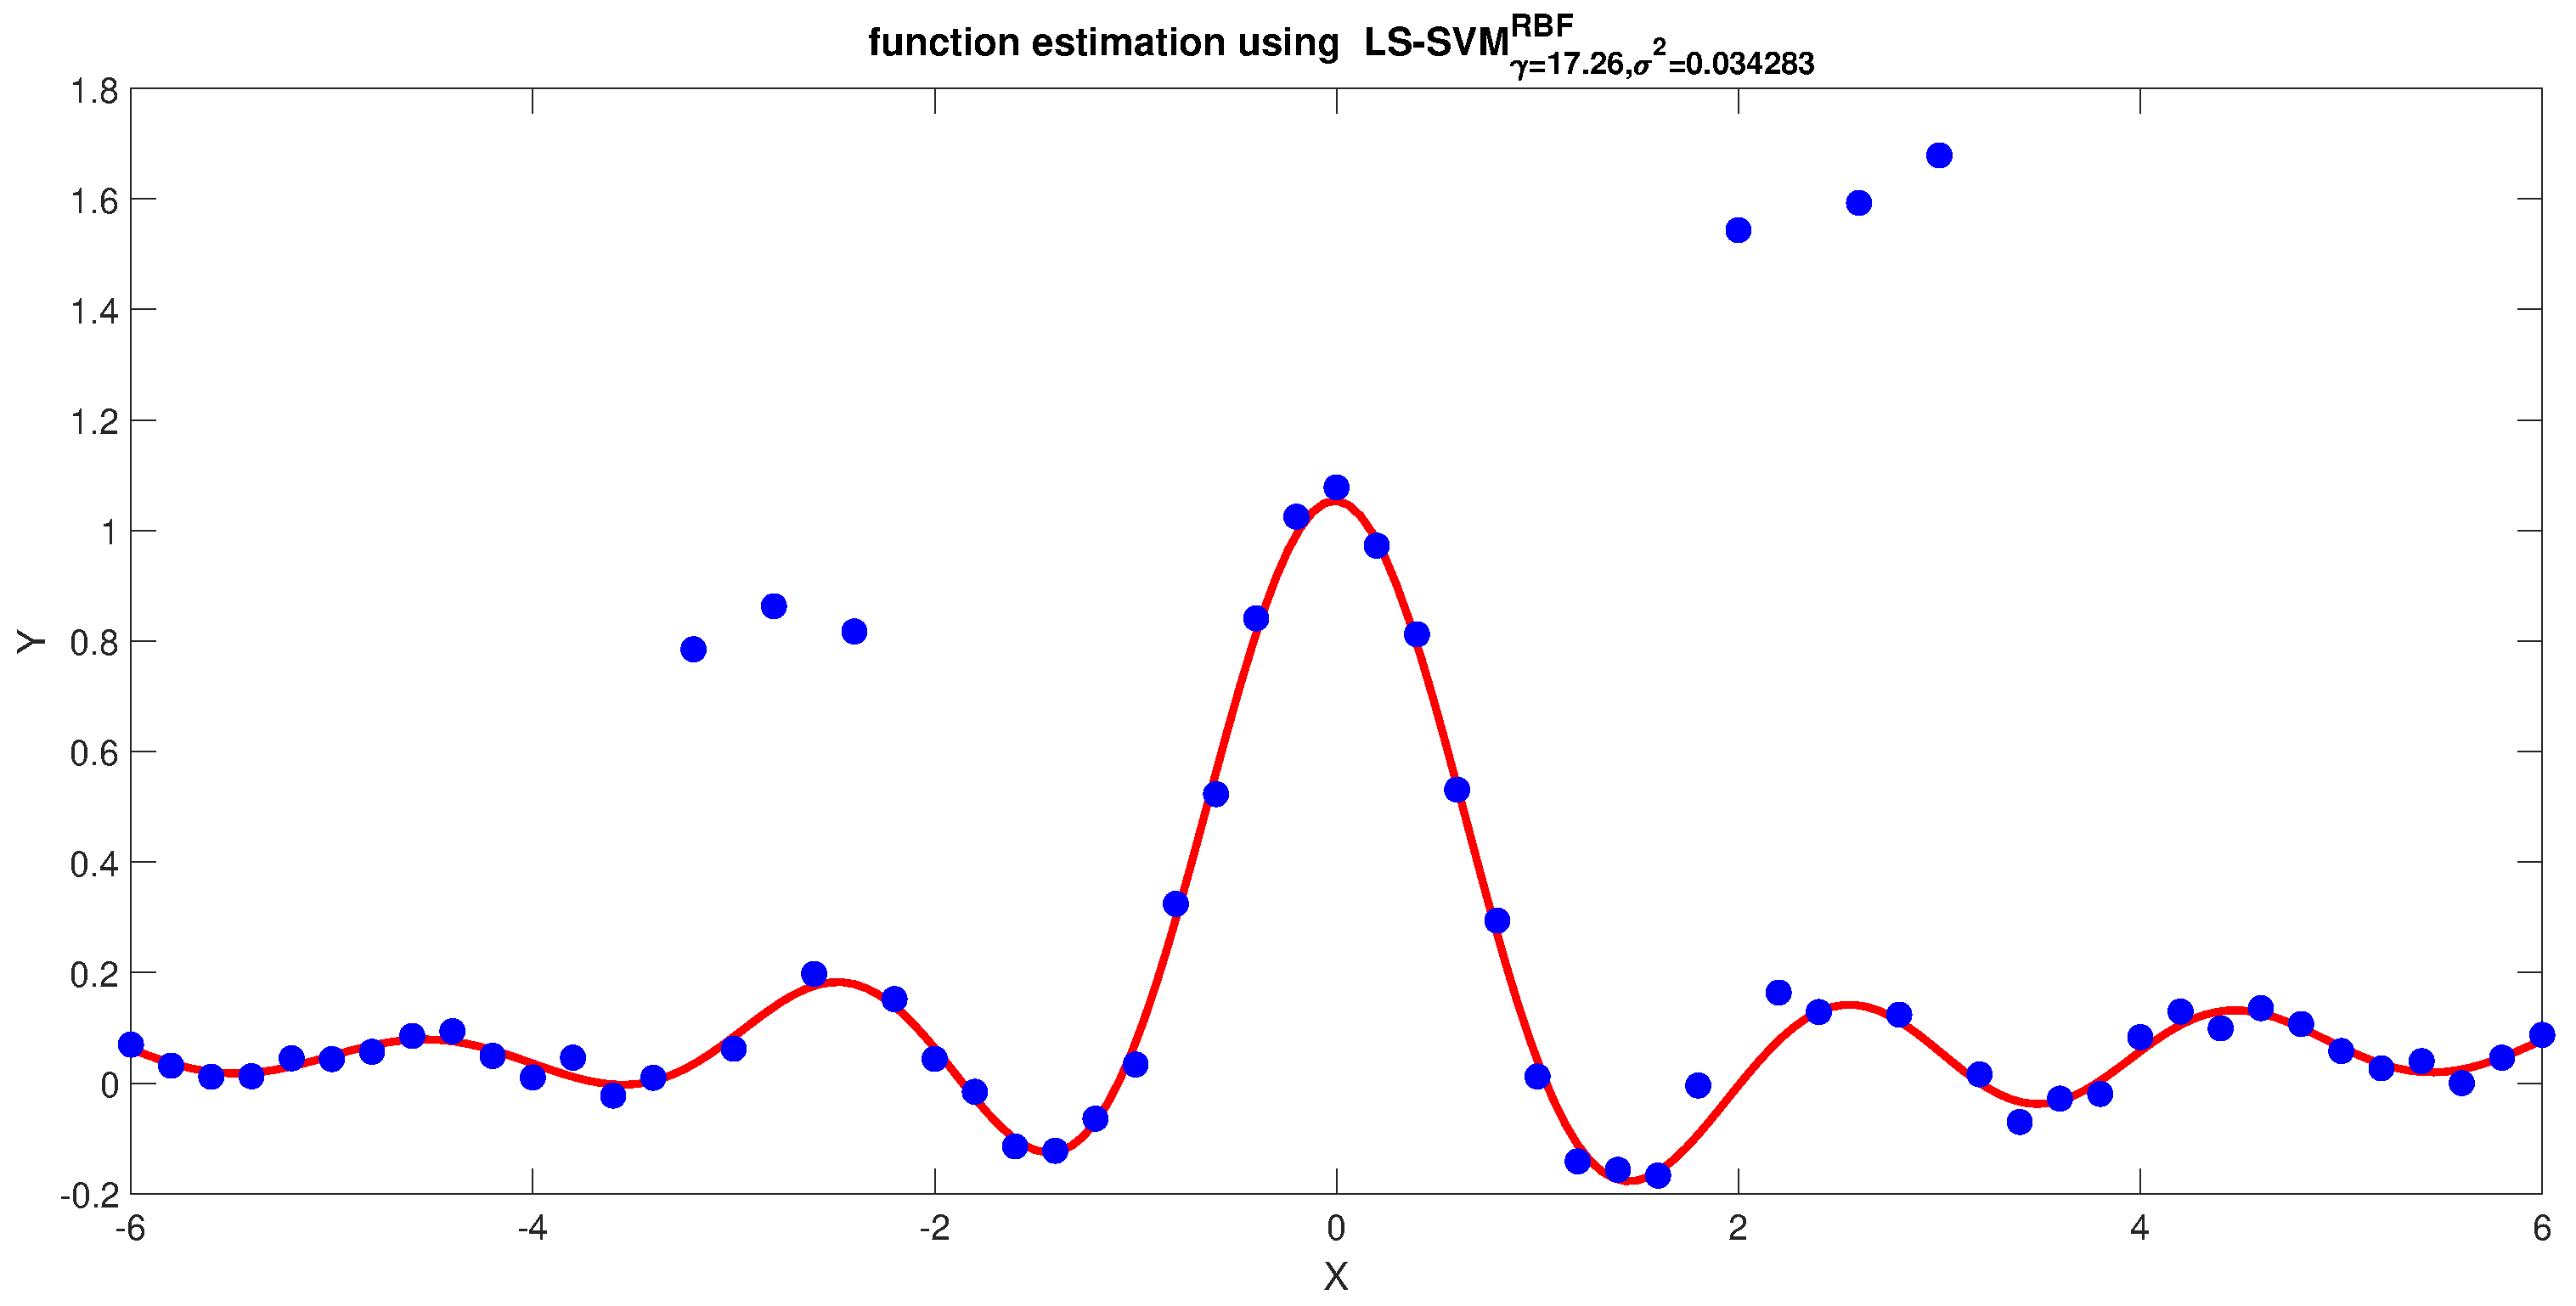
\includegraphics[height=.65\linewidth, width=0.9\linewidth]{Exercise2/Report/robust_hampel}
		\caption{Robust LS-SVM Regressor : Hampel}
		\label{fig:rob_hampel}
	\end{subfigure}
	\caption{LS-SVM : Robust versions with different weighting functions}
	\label{fig:robust_versions}
\end{figure}
\begin{table}[!htpb]
	\centering
	\begin{tabular}{ |p{4.5cm}||p{2.5cm}||p{2.5cm}||p{2.5cm}||p{2.5cm}|}
		\hline
		\cellcolor{blue!25} Weighting Function &\cellcolor{blue!25}$\gamma$ &\cellcolor{blue!25}$\sigma^2$ & \cellcolor{blue!25} Iterations for convergence & \cellcolor{blue!25} Cost \\ \hline
		\cellcolor{blue!25} wHuber  &12190.9097 & 0.10022 & 112 & 1.368683e-01 \\ \hline
		\cellcolor{blue!25} wLogistic &101.6236 & 0.081962 & 62&1.392045e-01  \\ \hline
		\cellcolor{blue!25} wMyriad & 11.4796&0.025126 & 13& 1.339679e-01 \\ \hline
		\cellcolor{blue!25} wHampel & 17.26 & 0.034283 & 4 & 1.360631e-01 \\ \hline
	\end{tabular}
	\caption{LS-SVM Robust Regressor with different weighting functions and their optimal hyper parameters ($\gamma$;$\sigma^2$)}
	\label{table:11}
\end{table}

The estimations of robust LS-SVM for various weighting functions are plotted in figure \ref{fig:robust_versions} and the results are given in the table \ref{table:11}. From the table \ref{table:11}, it can be seen that Hampel is faster as it achieves the convergence with only 4 iterations and Huber is the slowest. But, as seen from cost, the overall performance of all the weighting functions remain same. Every model gives approximately same estimations over the training data ignoring the outliers.
\section{Homework Problems}
\subsection{Logmap dataset}

\begin{wrapfigure}{L}{0.5\textwidth}
	\begin{center}
		\includegraphics[height=0.5\linewidth,width= 1\linewidth]{Exercise2/Report/HWOriginal.eps} 
		\caption{LS-SVM: Logmap Dataset with ($\gamma$;$\sigma^2$)=(10;10)}
		\label{fig:hw1}
	\end{center}
\end{wrapfigure}
In this section, we follow the instructions given in the exercise to obtain a model fit on the logmap dataset. From figure \ref{fig:hw1} it can be noticed that for initial ($\gamma$;$\sigma^2$) values of (10;10), the model estimates are very poor. The predictions fit the ground truth data only between the range 22 to 30. To get better model performance we use auto tune methods and cross validation method to obtain the optimal hyper parameters ($\gamma$;$\sigma^2$). For the lag parameter, we try out a range from 1 to 50 with each of the obtained optimal ($\gamma$;$\sigma^2$) pairs. The best fit obtained from the model is plotted in the figure \ref{fig:hw2}. The optimal values of ($\gamma$;$\sigma^2$) and the lag is chosen by calculating MAE of the model on the test set for which the MAE $\leq$ 15. The model estimates are not completely perfect as it fails to fit at the huge peaks of the data set. The plots shown in figure \ref{fig:hw2} are the ones with the least MAE values.
\begin{figure}[!ht] 
	\begin{subfigure}{.5\textwidth}
		\centering
		\captionsetup{width=0.8\linewidth}
		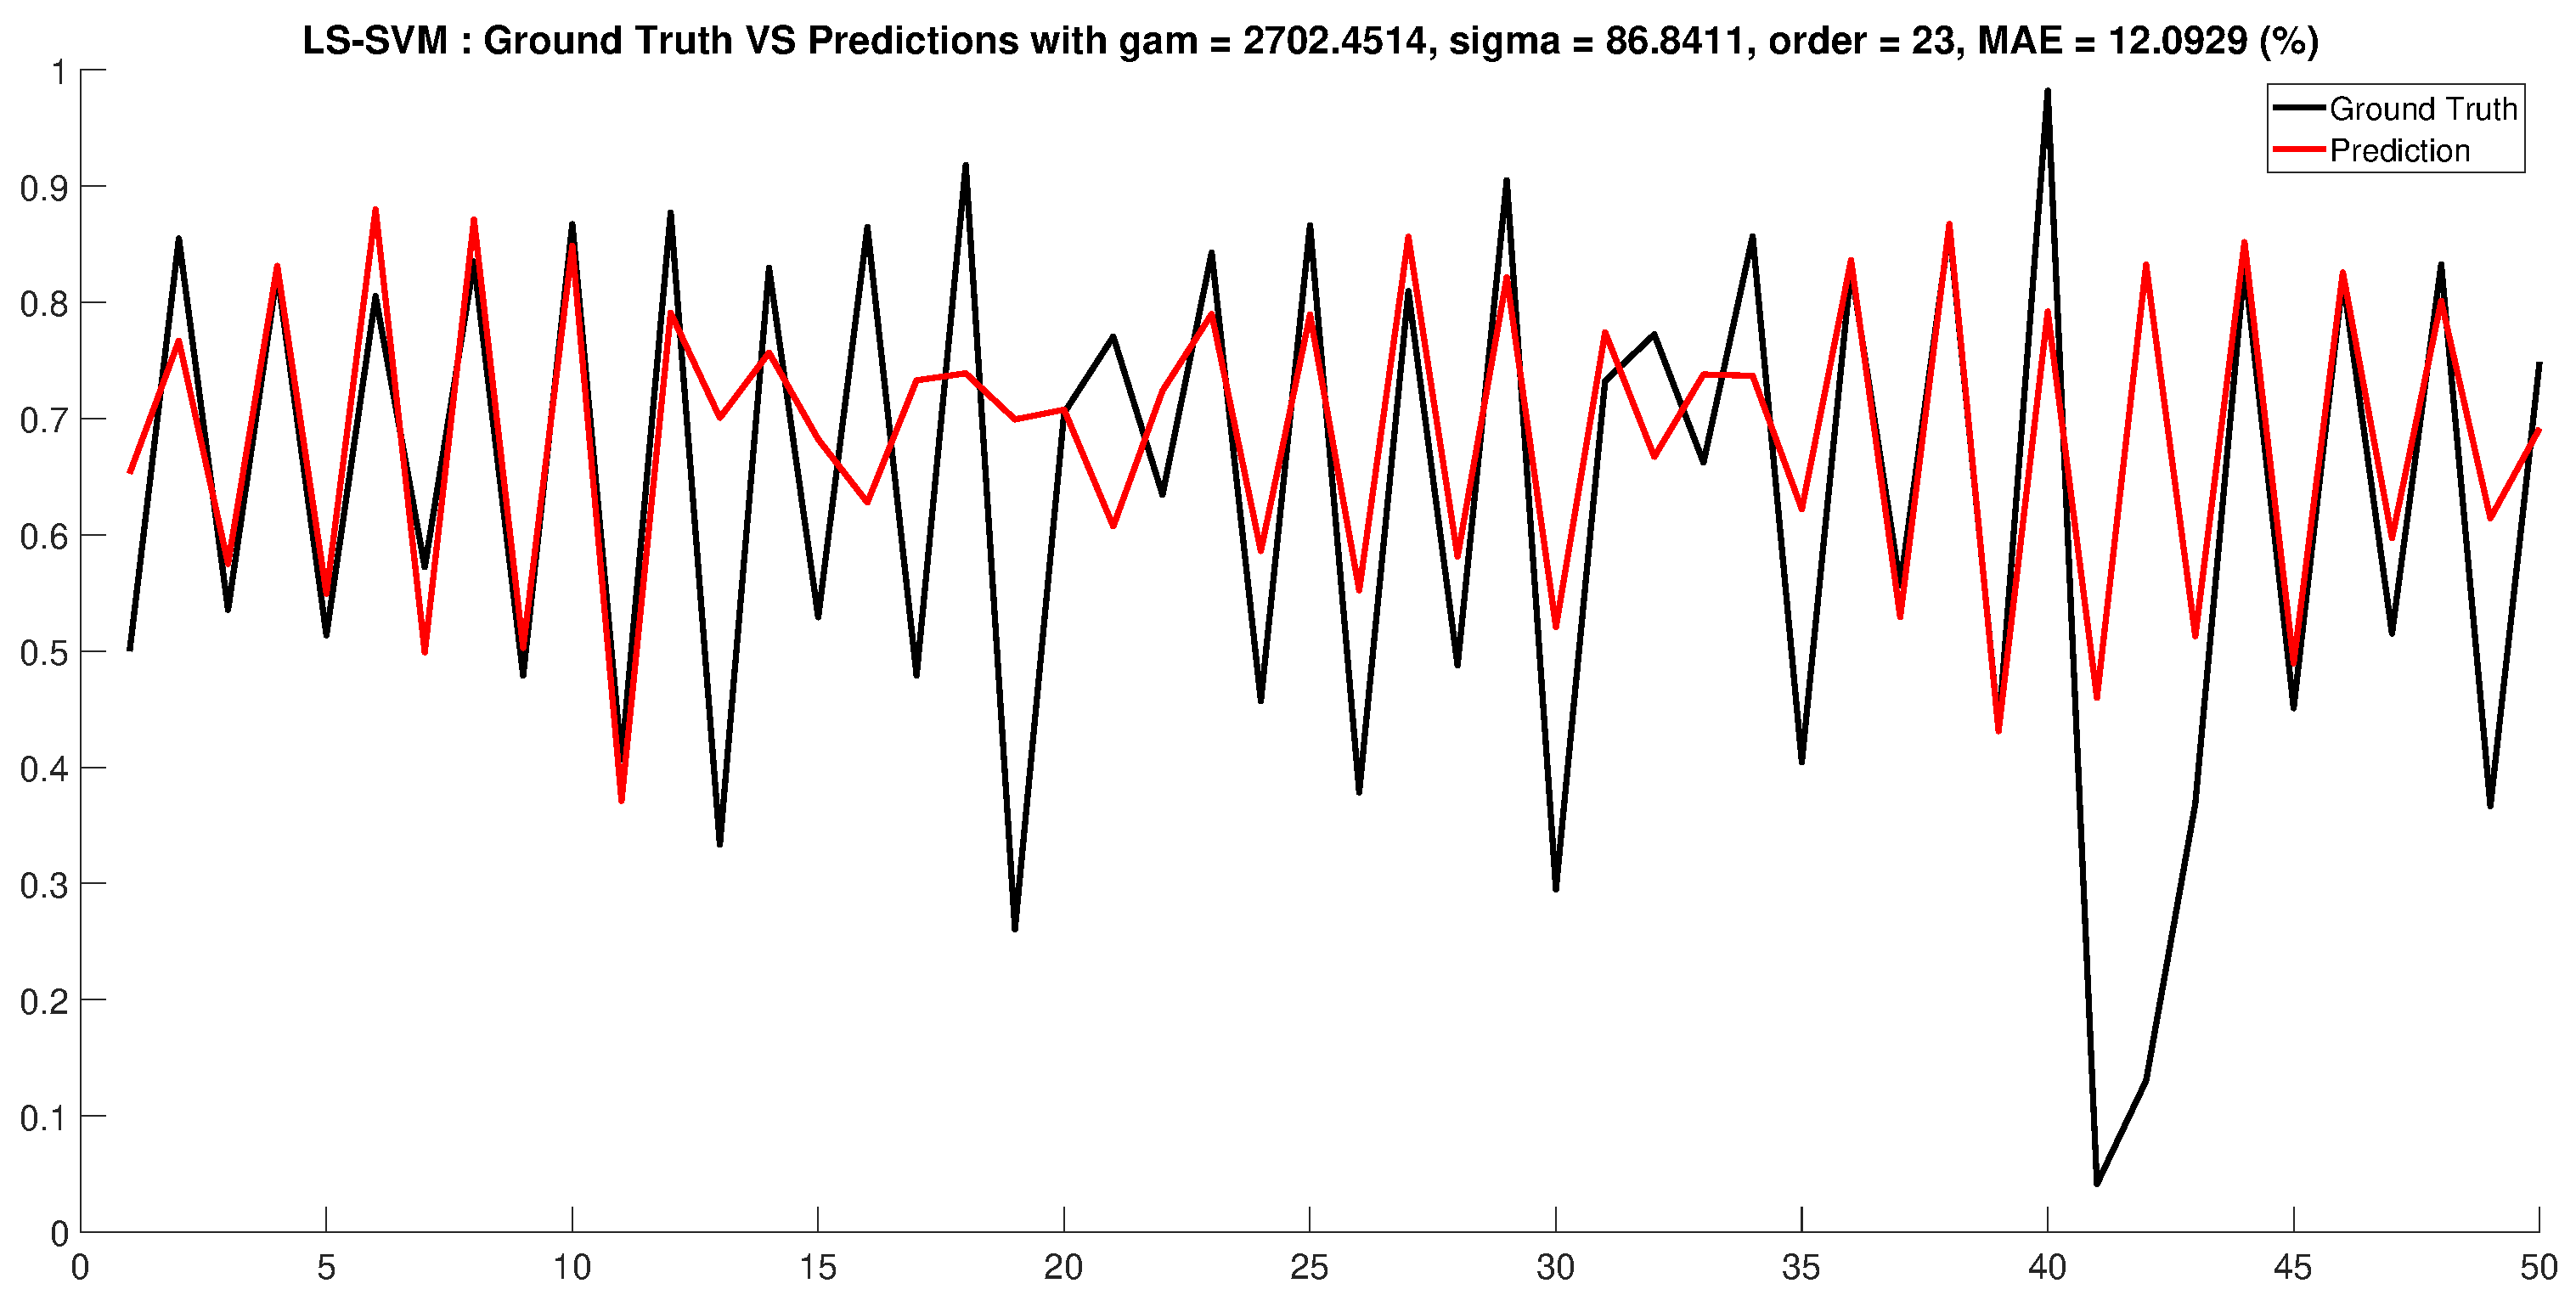
\includegraphics[height=.5\linewidth, width=0.85\linewidth]{Exercise2/Report/Hw_tuned1}
		\caption{LogMap: LS-SVM Regressor with optimal ($\gamma$;$\sigma^2$)=(2702.4514 ; 86.8411), lag = 23 and MAE = 12.09(\%)}
		\label{fig:hw_tuned1}
	\end{subfigure}%
	\begin{subfigure}{.5\textwidth}
		\centering
		\captionsetup{width=0.8\linewidth}
		\includegraphics[height=.5\linewidth, width=0.85\linewidth]{Exercise2/Report/Hw_tuned3}
		\caption{LogMap : LS-SVM Regressor with optimal ($\gamma$;$\sigma^2$)=(11029.3131 ; 269.0996), lag = 23 and MAE = 12.5799(\%)}
		\label{fig:hw_tuned2}
	\end{subfigure}
\caption{LS-SVM: Logmap Dataset with optimally tuned hyper parameters}
\label{fig:hw2}
\end{figure}
\subsection{Santa Fe dataset}
\textbf{Does order = 50 for the utilized auto-reressive model sounds like a good choice?}

The data set contains 1000 training and 200 test points. In time-series prediction, the future values are predicted based on the past values during the function estimation. This is known as a auto-regressive model. The prder/lag in this model determines the numbers of samples/period away from which the prediction is to be made which means the prediction starts after lag number of points. With the setting of lag = 50, the model gives a decent performance initially but later, a small shift is seen between the actual and predicted data set in figure \ref{fig:sfe1}. The order 50 seems like a good choice, but the model performance can still be improved by reducing its value. \\
\begin{wrapfigure}{L}{0.5\textwidth}
	\begin{center}
		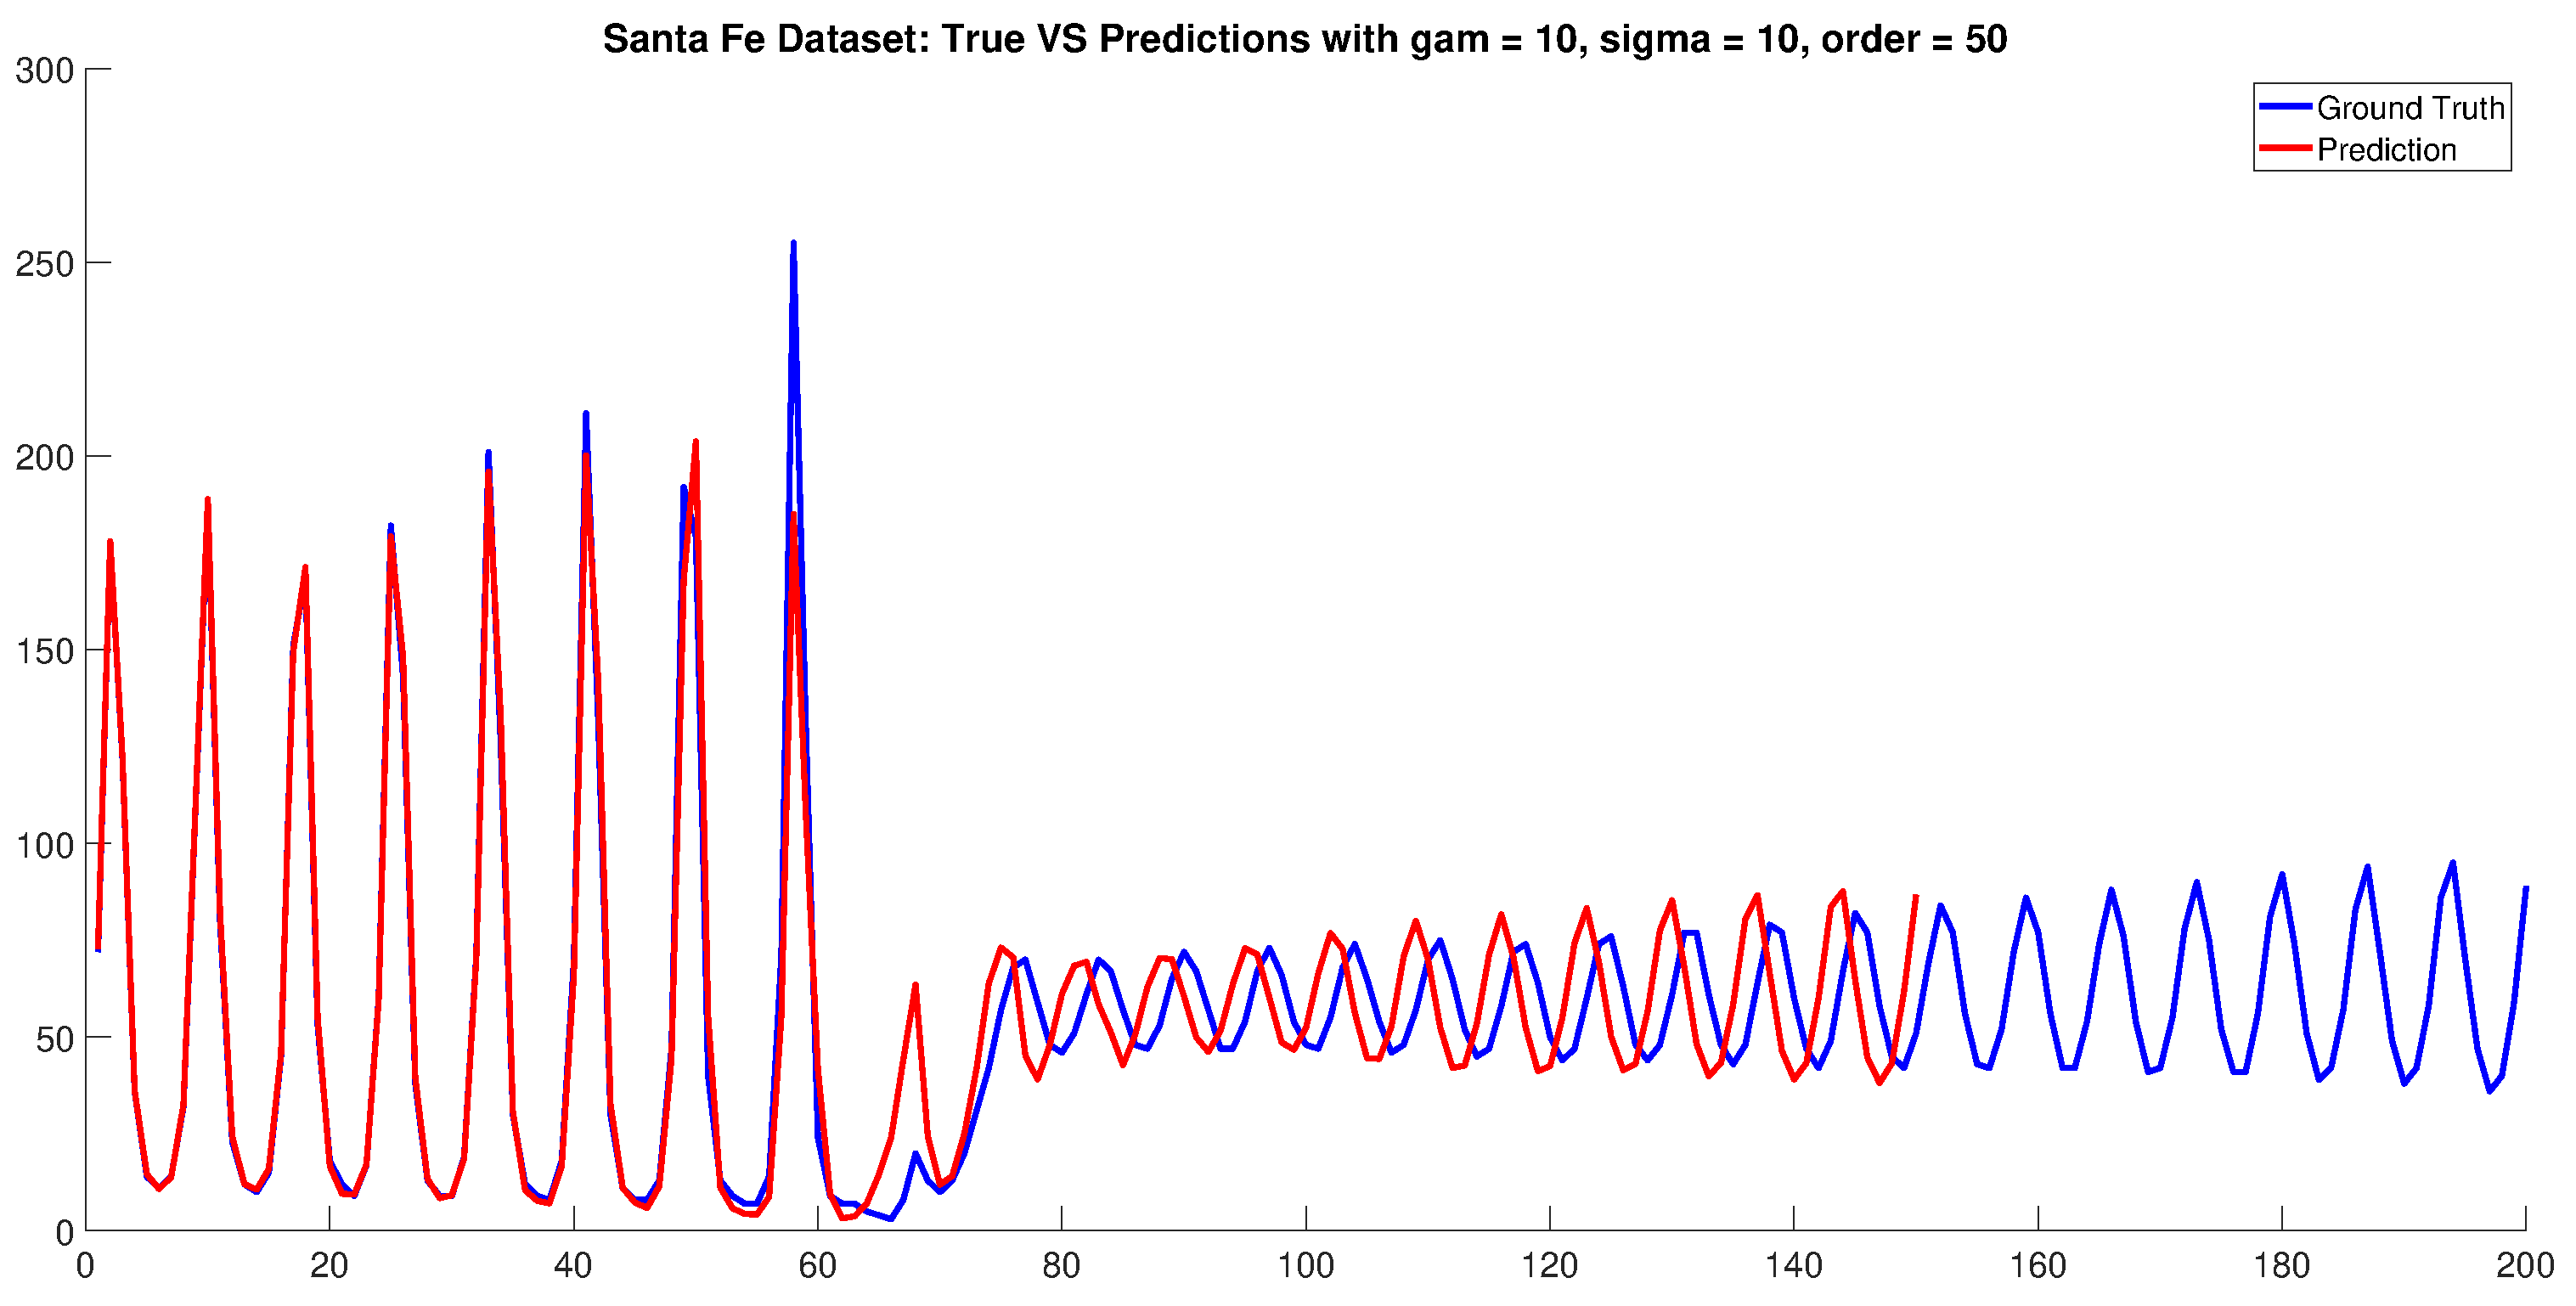
\includegraphics[height=0.5\linewidth,width= 1\linewidth]{Exercise2/Report/sfe1} 
		\caption{Santa Fe Dataset: ($\gamma$;$\sigma^2$)=(10,10) and Lag = 50}
		\label{fig:sfe1}
	\end{center}
\end{wrapfigure}
 
 \textbf{Would it be sensible to use the performance of this recurrent prediction on the validation set to optimize hyperparameters and the model order?}
 
 Yes, we can use the performance of this model to optimize the hyper parameters. We can divide the training set of 1000 points into say 700 training and 300 validation points. The validation set can be used for fine tuning the model parameters so that the model can perform better on the test set.\\\\
 \textbf{Tune the parameters (order, gam and sig2) and do time series prediction.}

 The model is tuned with optimal hyper parameters obtained from \textit{tunelssvm} over a range of order/lag values 1-50. MAE values are calculated for the corresponding order and ($\gamma$;$\sigma^2$) pairs. The plot \ref{fig:sfe2} shows the model with least MAE value which is obtained for a lag of 22. It can be seen that the model gives good estimate for the larger peaks of the dataset and poor estimates in the later part. Figure \ref{fig:sfe3} shows MAE's calculated over the range of order/lag. 
 \begin{figure}[!ht] 
 	\begin{subfigure}{.5\textwidth}
 		\centering
 		\captionsetup{width=0.8\linewidth}
 		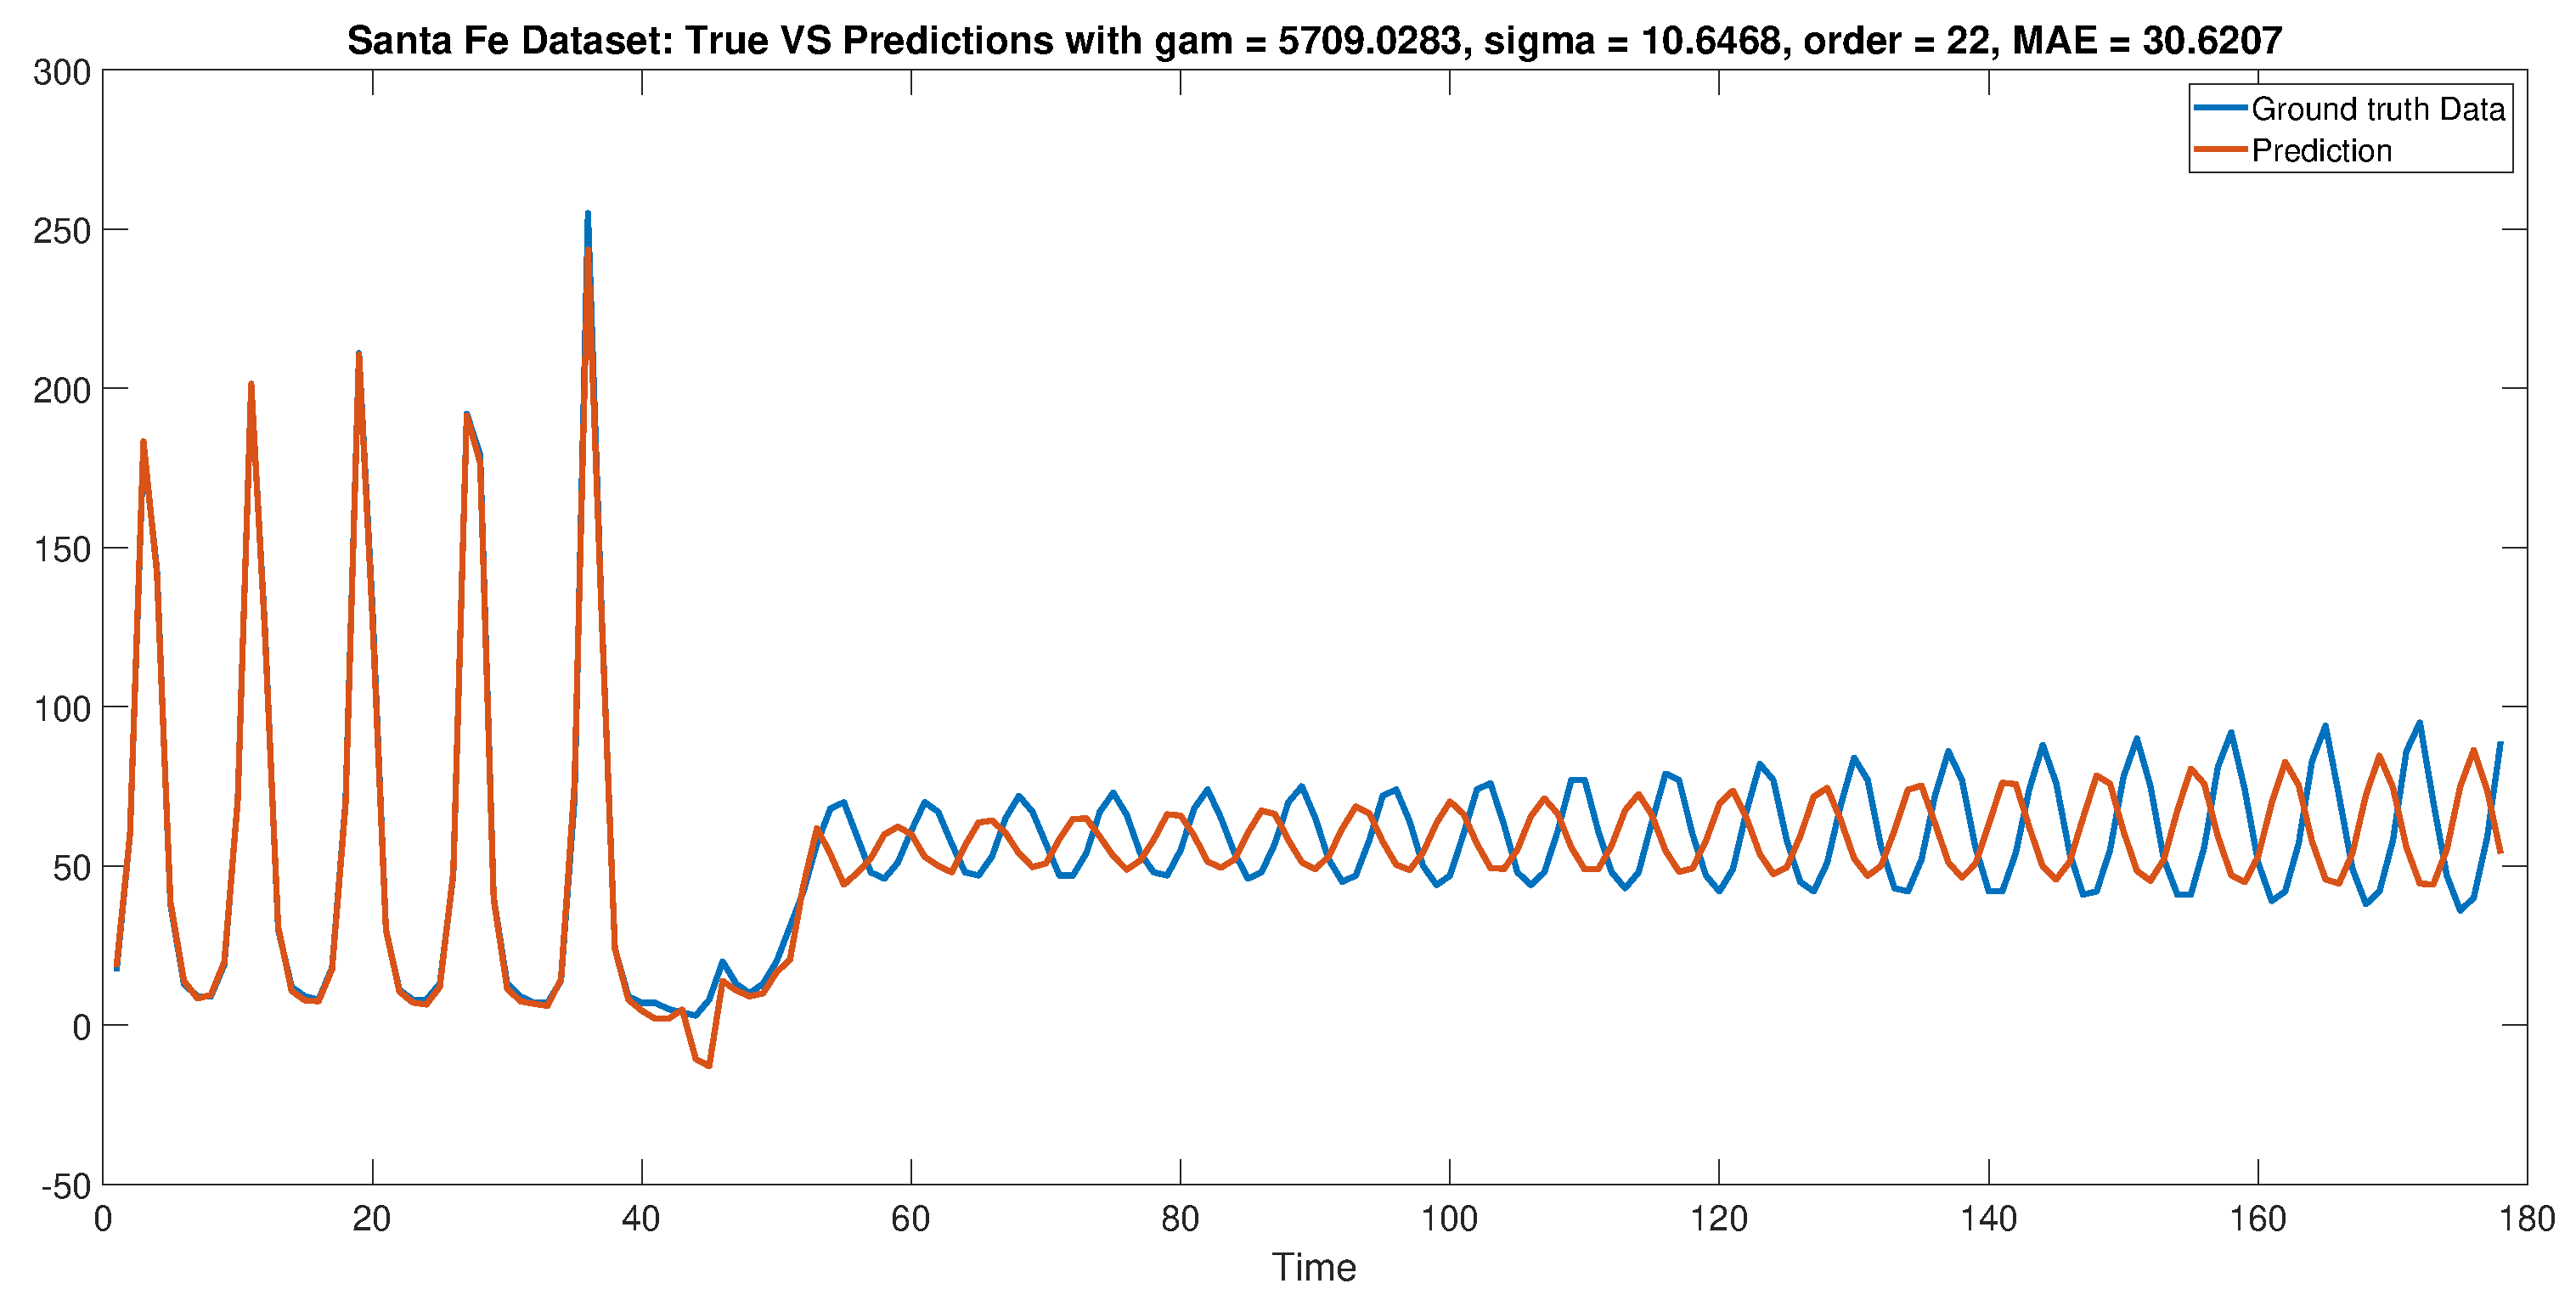
\includegraphics[height=.5\linewidth, width=0.85\linewidth]{Exercise2/Report/sfe2}
 		\caption{Santa Fe Dataset: ($\gamma$;$\sigma^2$) = (5709.0283 ; 10.6468) and MAE = 30.6207(\%)}
 		\label{fig:sfe2}
 	\end{subfigure}%
 	\begin{subfigure}{.5\textwidth}
 		\centering
 		\captionsetup{width=0.8\linewidth}
 		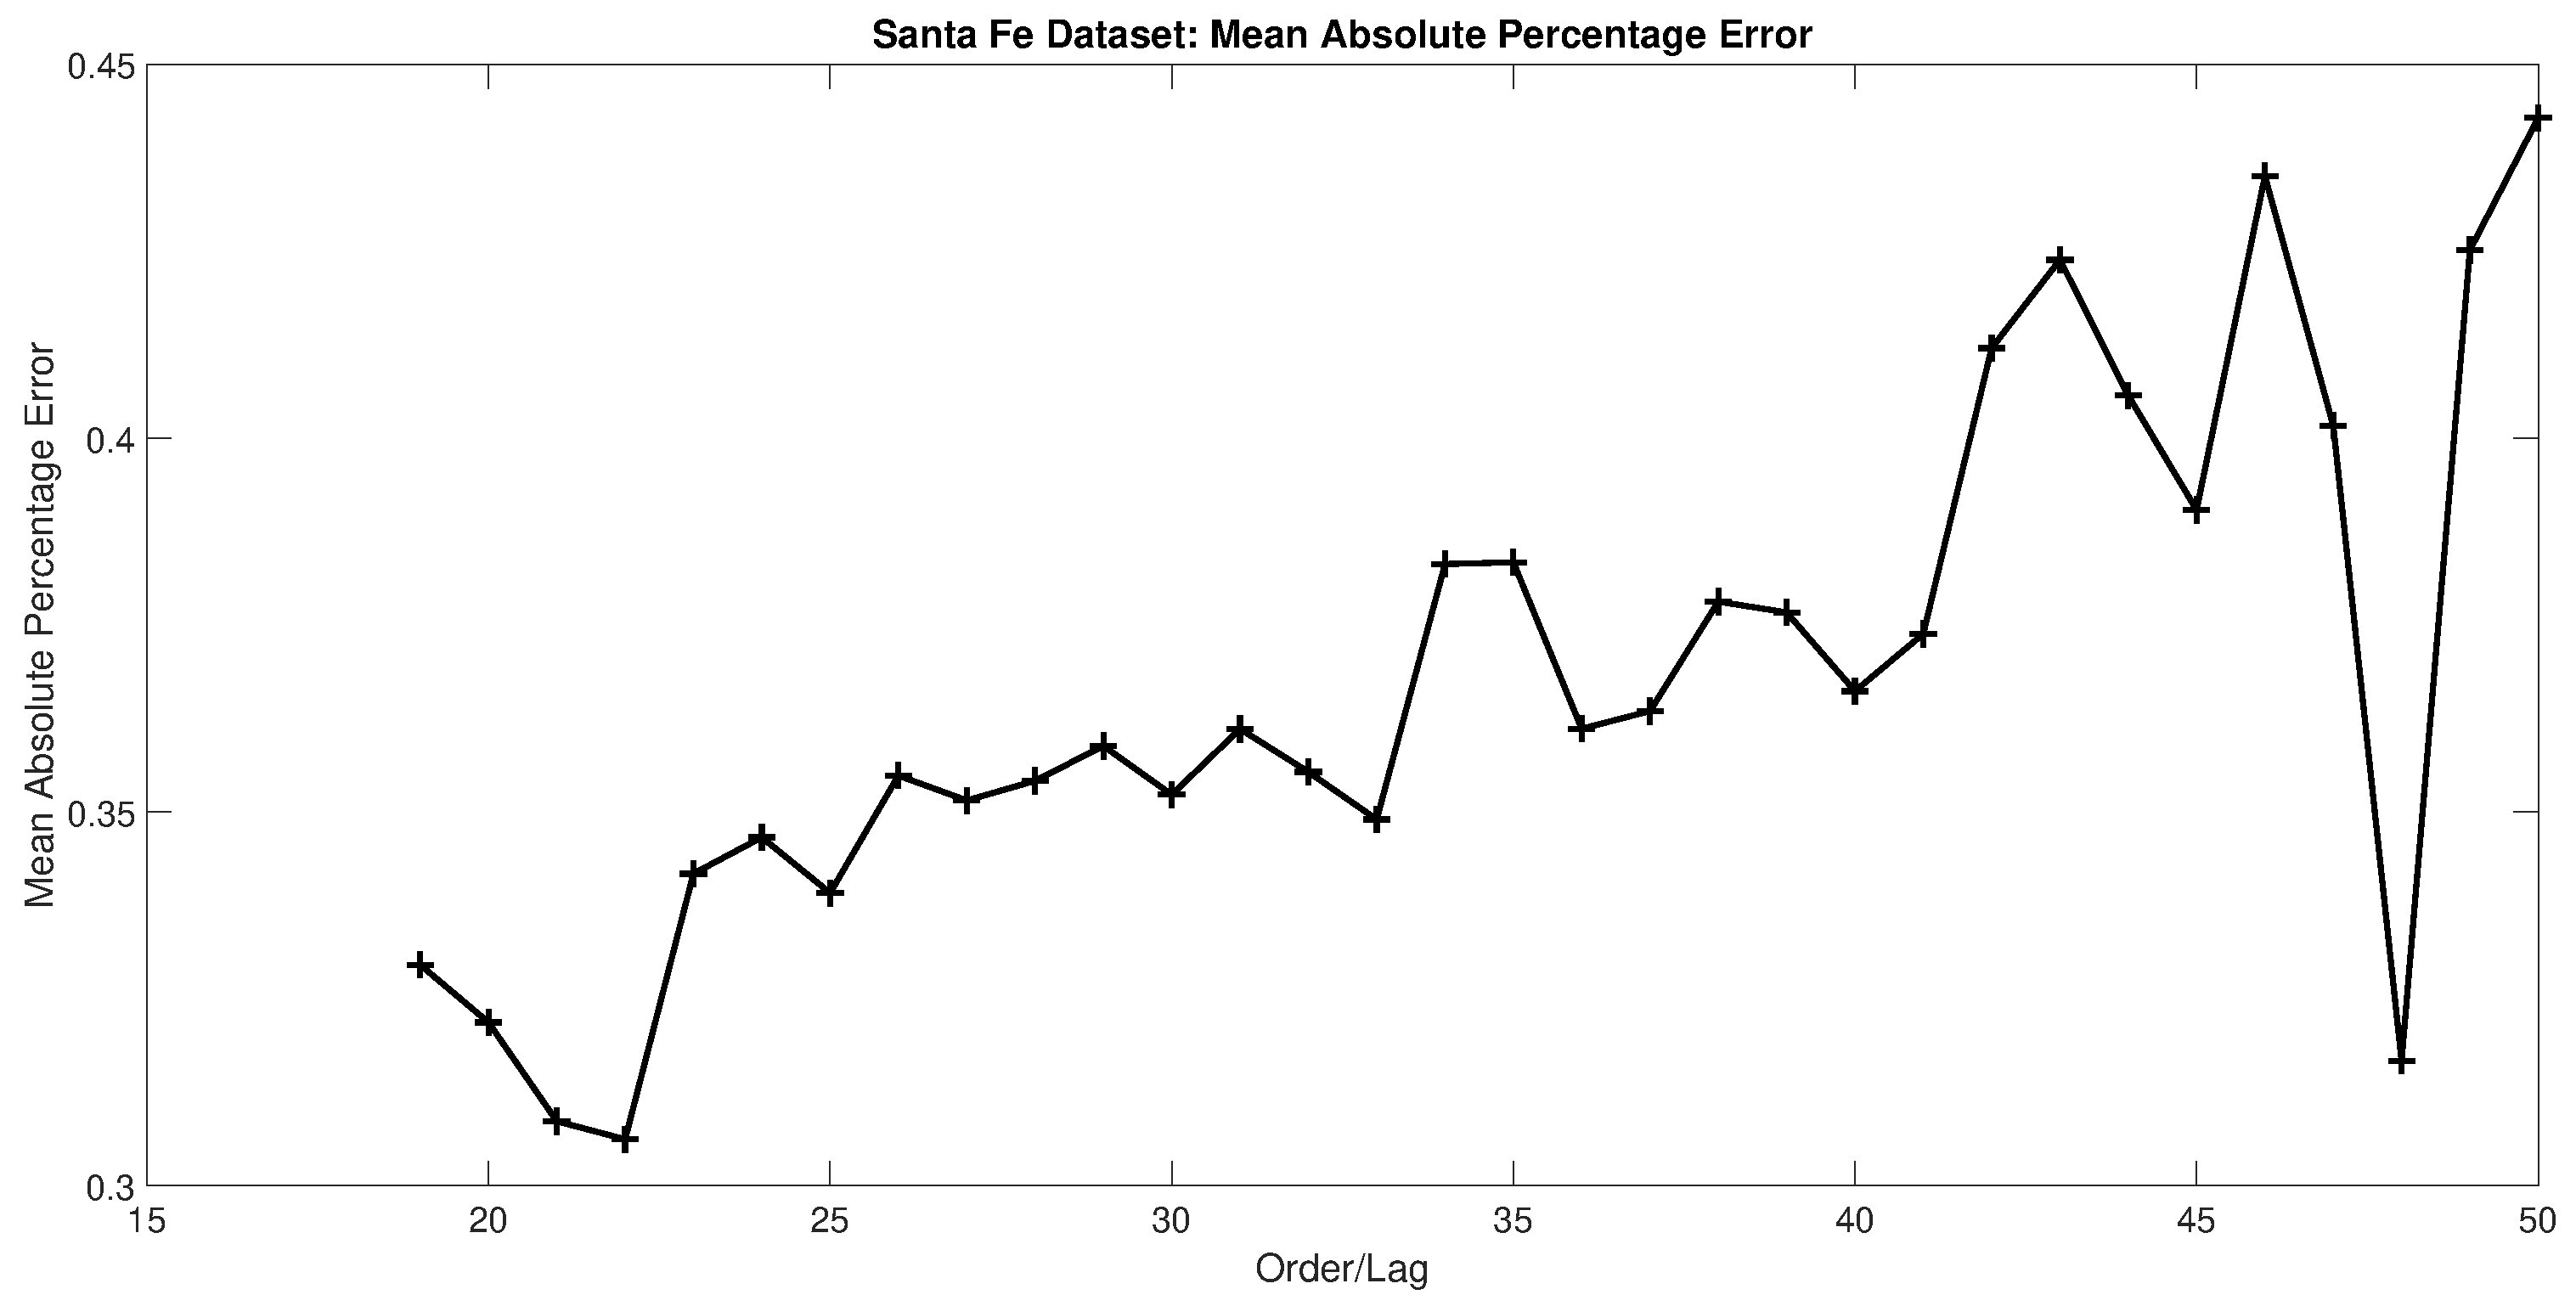
\includegraphics[height=.5\linewidth, width=0.85\linewidth]{Exercise2/Report/sfe3}
 		\caption{Santa Fe Dataset : MAPE for optimal ($\gamma$;$\sigma^2$) over a range of order/lag values}
 		\label{fig:sfe3}
 	\end{subfigure}
 	\caption{Santa Fe Dataset: Best Fit with optimal hyper parameters and corresponding MAPE for the tuned ($\gamma$;$\sigma^2$) pairs}
 	\label{fig:sfe}
 \end{figure}